\clearpage
%%%%%%%%%%%%%%%%%%%%%%%%%%%%%%%%%%%%%
\section{Signal modeling}
%\textbf {editors: Felipe Silva}
%SIGNAL MODELING...  % to be commented

Along the same lines as the background modeling (Section \ref{sec:background_modeling}), the signal modeling is implemented as a two dimensional unbinned maximum likelihood fit on the $m_{\mu\mu}$ and the $m_{\mu\mu\gamma}$ invariant masses distributions, but this time, only using the signal simulated MC samples~\ref{sec:datasets}. Since, for the two spectra, it is expected a peak-like distribution, one centered in the \Z (or Higgs) boson mass and the other centered in the $\Upsilon$ mass, two also peak-like analytics \textit{pdfs} were chosen to compose the signal model. The modeling is summarized in table \ref{tab:SignalModeling}.


% % signal modeling
% \begin{table}[ht]
% \begin{center}
% \begin{tabular}{l|c|c}
%                          & \boldmath$M_{\mu\mu}$                                          & \boldmath$M_{\mu\mu\gamma}$       \\ \hline 
% \textbf{\boldmath$Z \rightarrow \Upsilon(1S,2S,3S) +\gamma$}       & Crystal Ball & Double Crystal Ball      \\ \hline
% \textbf{\boldmath$H \rightarrow \Upsilon(1S,2S,3S) +\gamma$} & Double Crystal Ball & Crystal Ball + Gaussian with the same mean  \\ 
% \end{tabular}

% \caption{Modeling for each signal source and mass component.}
% \label{tab:SignalModeling}
% \end{center}
% \end{table}


% signal modeling
\begin{table}[ht]
\begin{center}
\caption{Modeling for each signal source and mass component.}
\begin{tabular}{l|c|c}
                         & \boldmath$m_{\mu\mu}$                                          & \boldmath$m_{\mu\mu\gamma}$       \\ \hline 
\textbf{\boldmath$Z \rightarrow \Upsilon(nS) +\gamma$}       & Double Crystal Ball & Double Crystal Ball      \\ \hline
\textbf{\boldmath$H \rightarrow \Upsilon(nS) +\gamma$} & Double Crystal Ball & Crystal Ball + Gaussian (same mean)  \\ 
\end{tabular}

\label{tab:SignalModeling}
\end{center}
\end{table}




The projections of the modeling for the \Z boson decay channel analysis can be found at figures \ref{fig:ZToUpsilon_Signal_Cat0}, \ref{fig:ZToUpsilon_Signal_Cat1}, \ref{fig:ZToUpsilon_Signal_Cat2} and \ref{fig:ZToUpsilon_Signal_Cat3}, for Inclusive, EB High R9, EB Low R9 and EE, respectively. The projection on the modeling for the Higgs boson signal can be found at Figure \ref{fig:HToUpsilon_Signal_Cat0}. A deeper discussion on the systematics uncertainties associated to them, will be presented in the next section.



% Z To Upsilon - Signal Modeling
% Cat0
\begin{figure}[!htbp]
\begin{center}


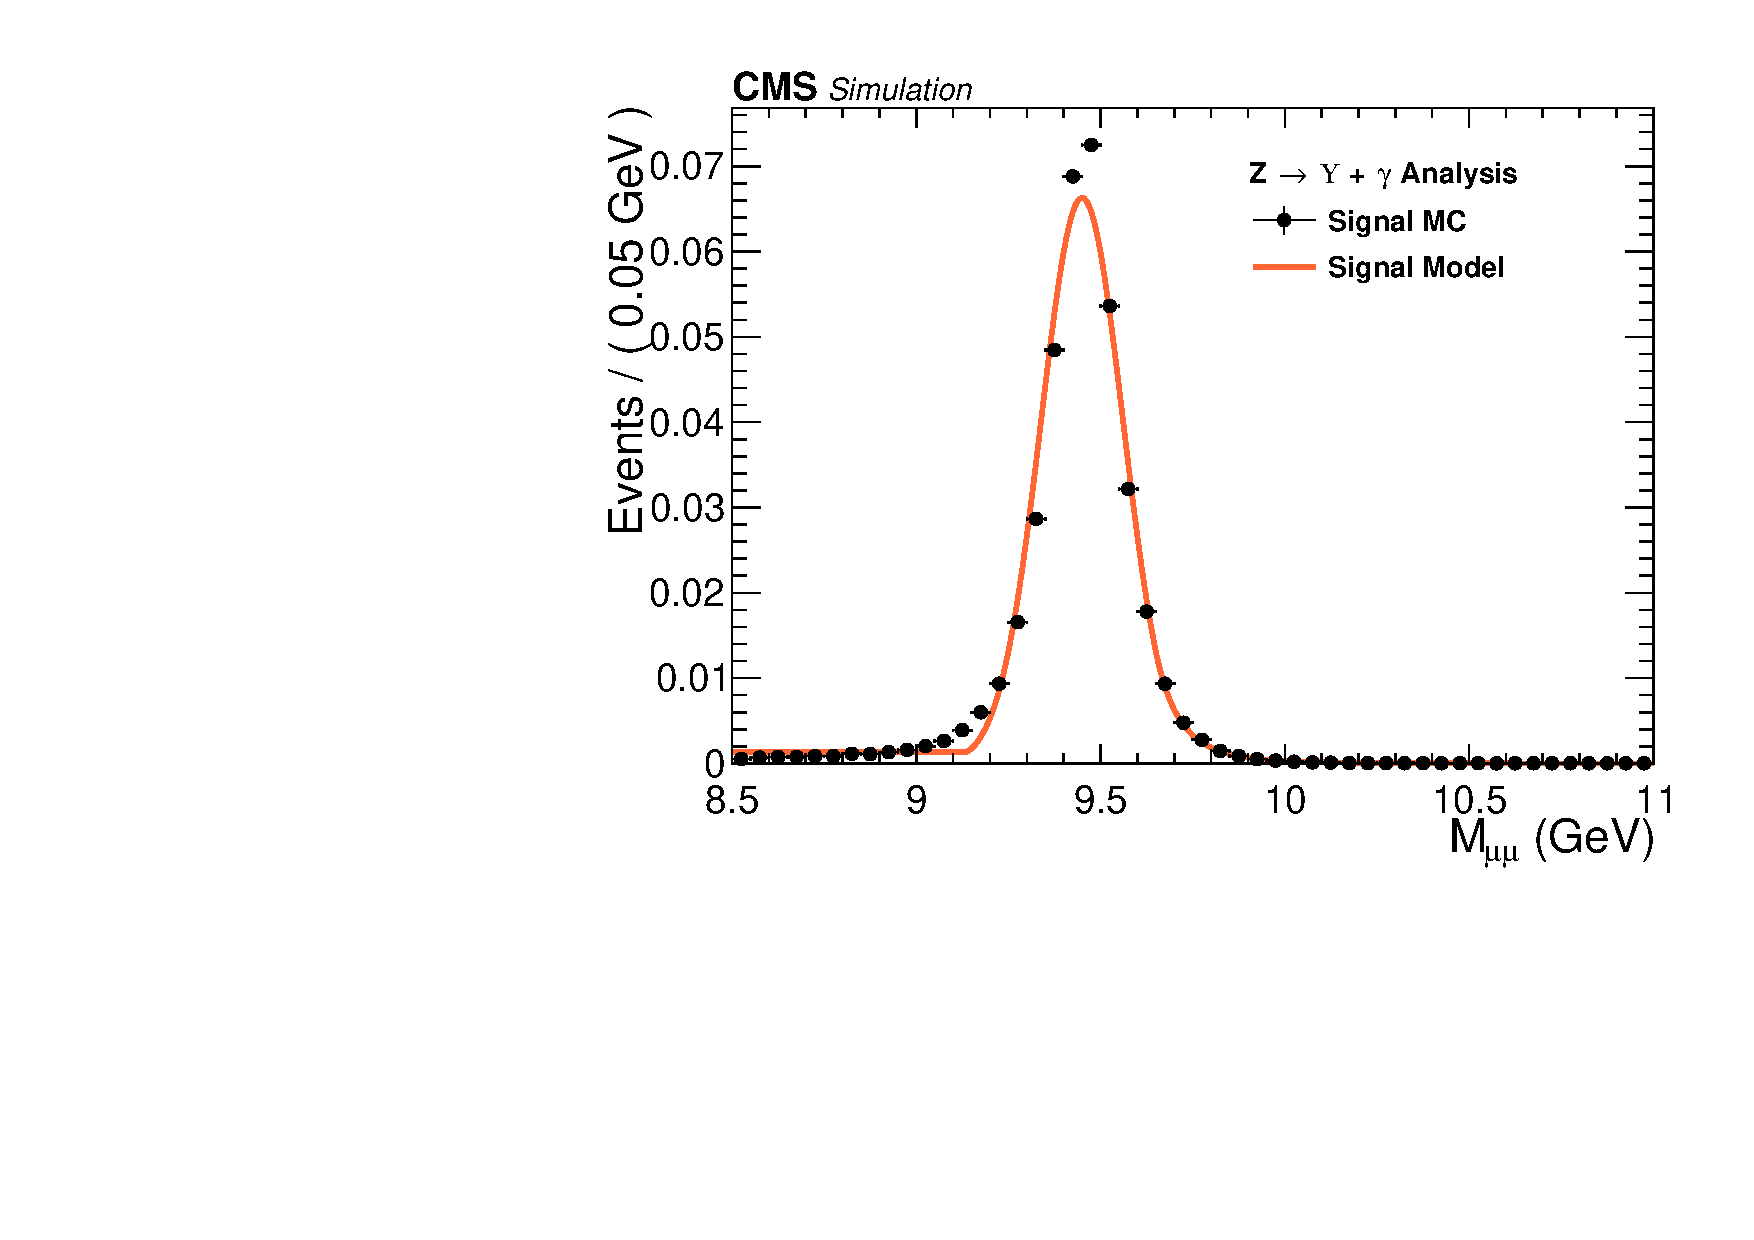
\includegraphics[width=0.45\textwidth]{figures_and_tables/fitPlotFiles2D/ZToUpsilonPhotonSignalAndBackgroundFit/mMuMNU_ZToUpsilon1SPhotonSignalAndBackgroundFit_Signal_Cat0}\hspace*{1.cm}
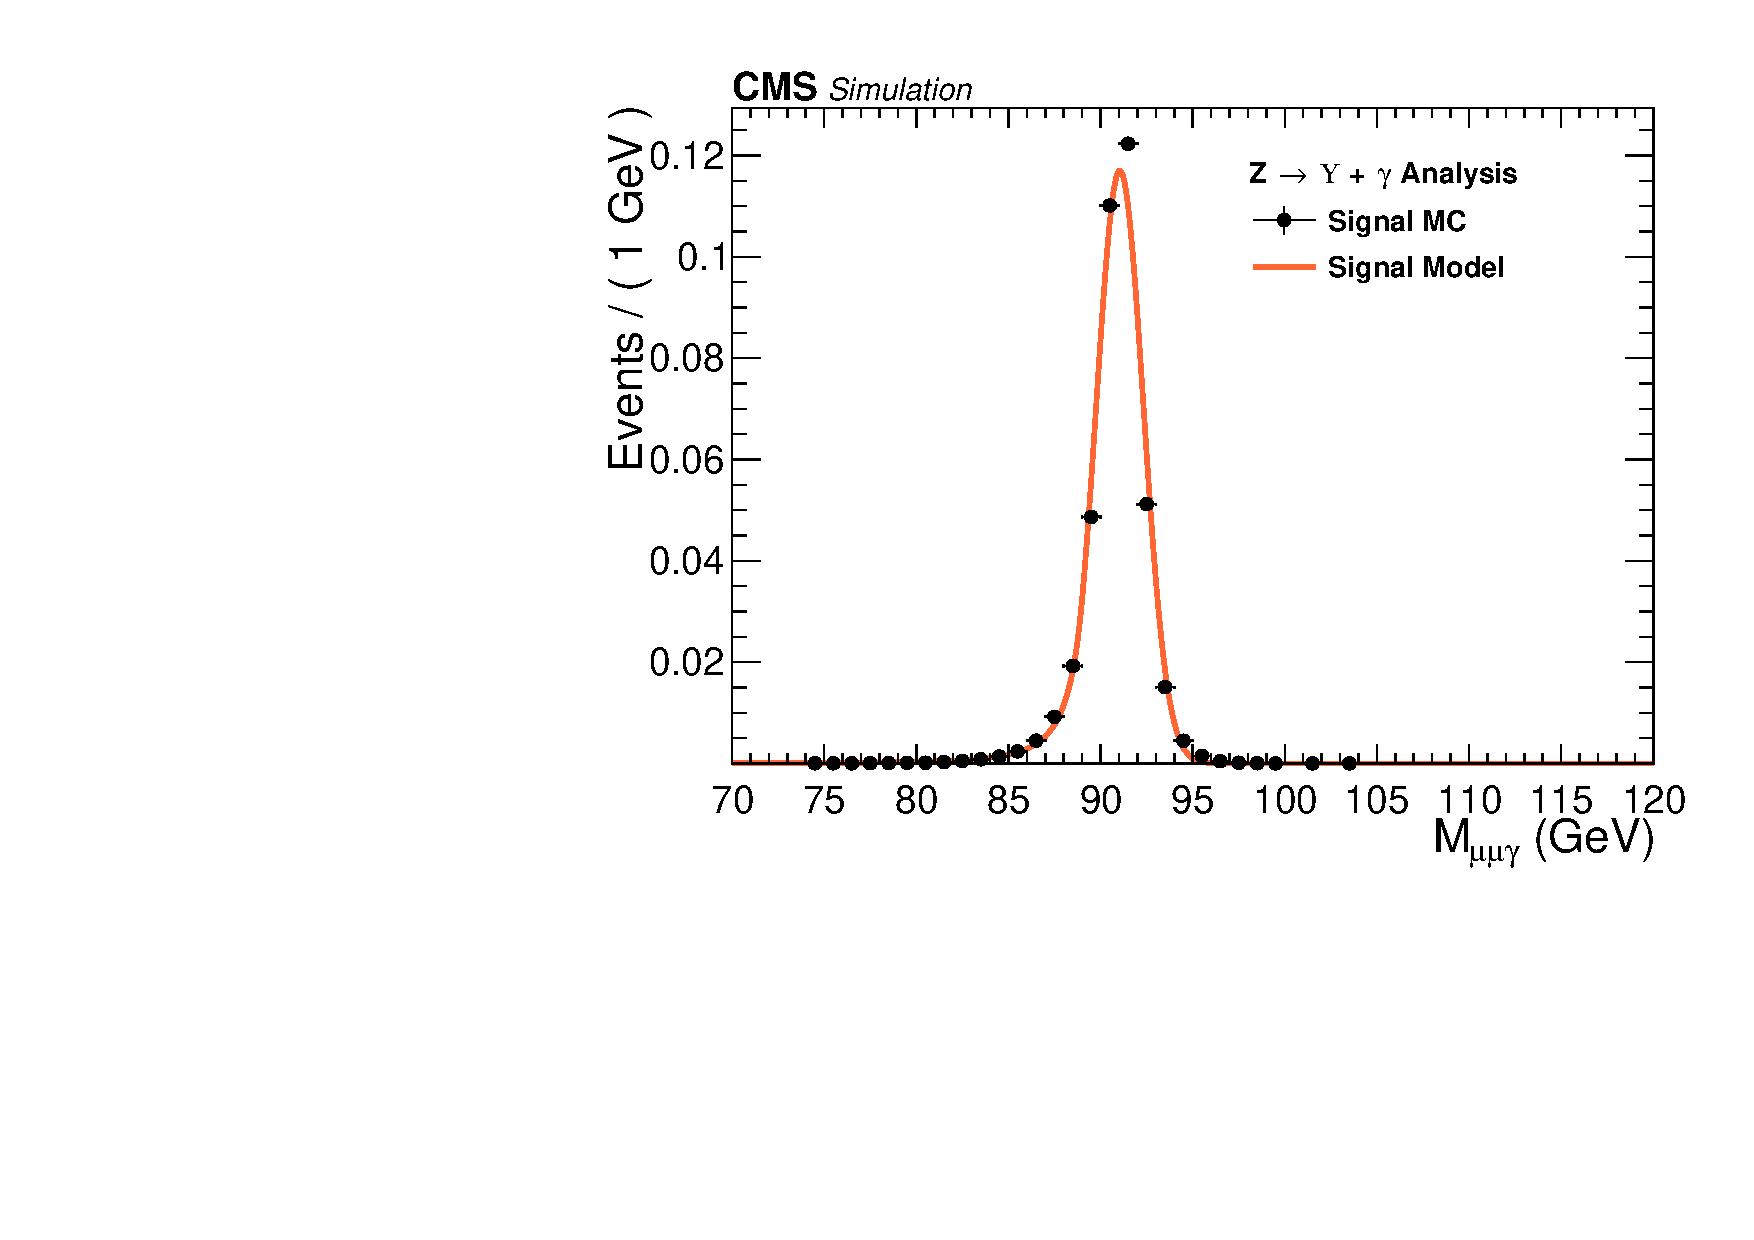
\includegraphics[width=0.45\textwidth]{figures_and_tables/fitPlotFiles2D/ZToUpsilonPhotonSignalAndBackgroundFit/mHZ_ZToUpsilon1SPhotonSignalAndBackgroundFit_Signal_Cat0_default}\hspace*{1.cm}

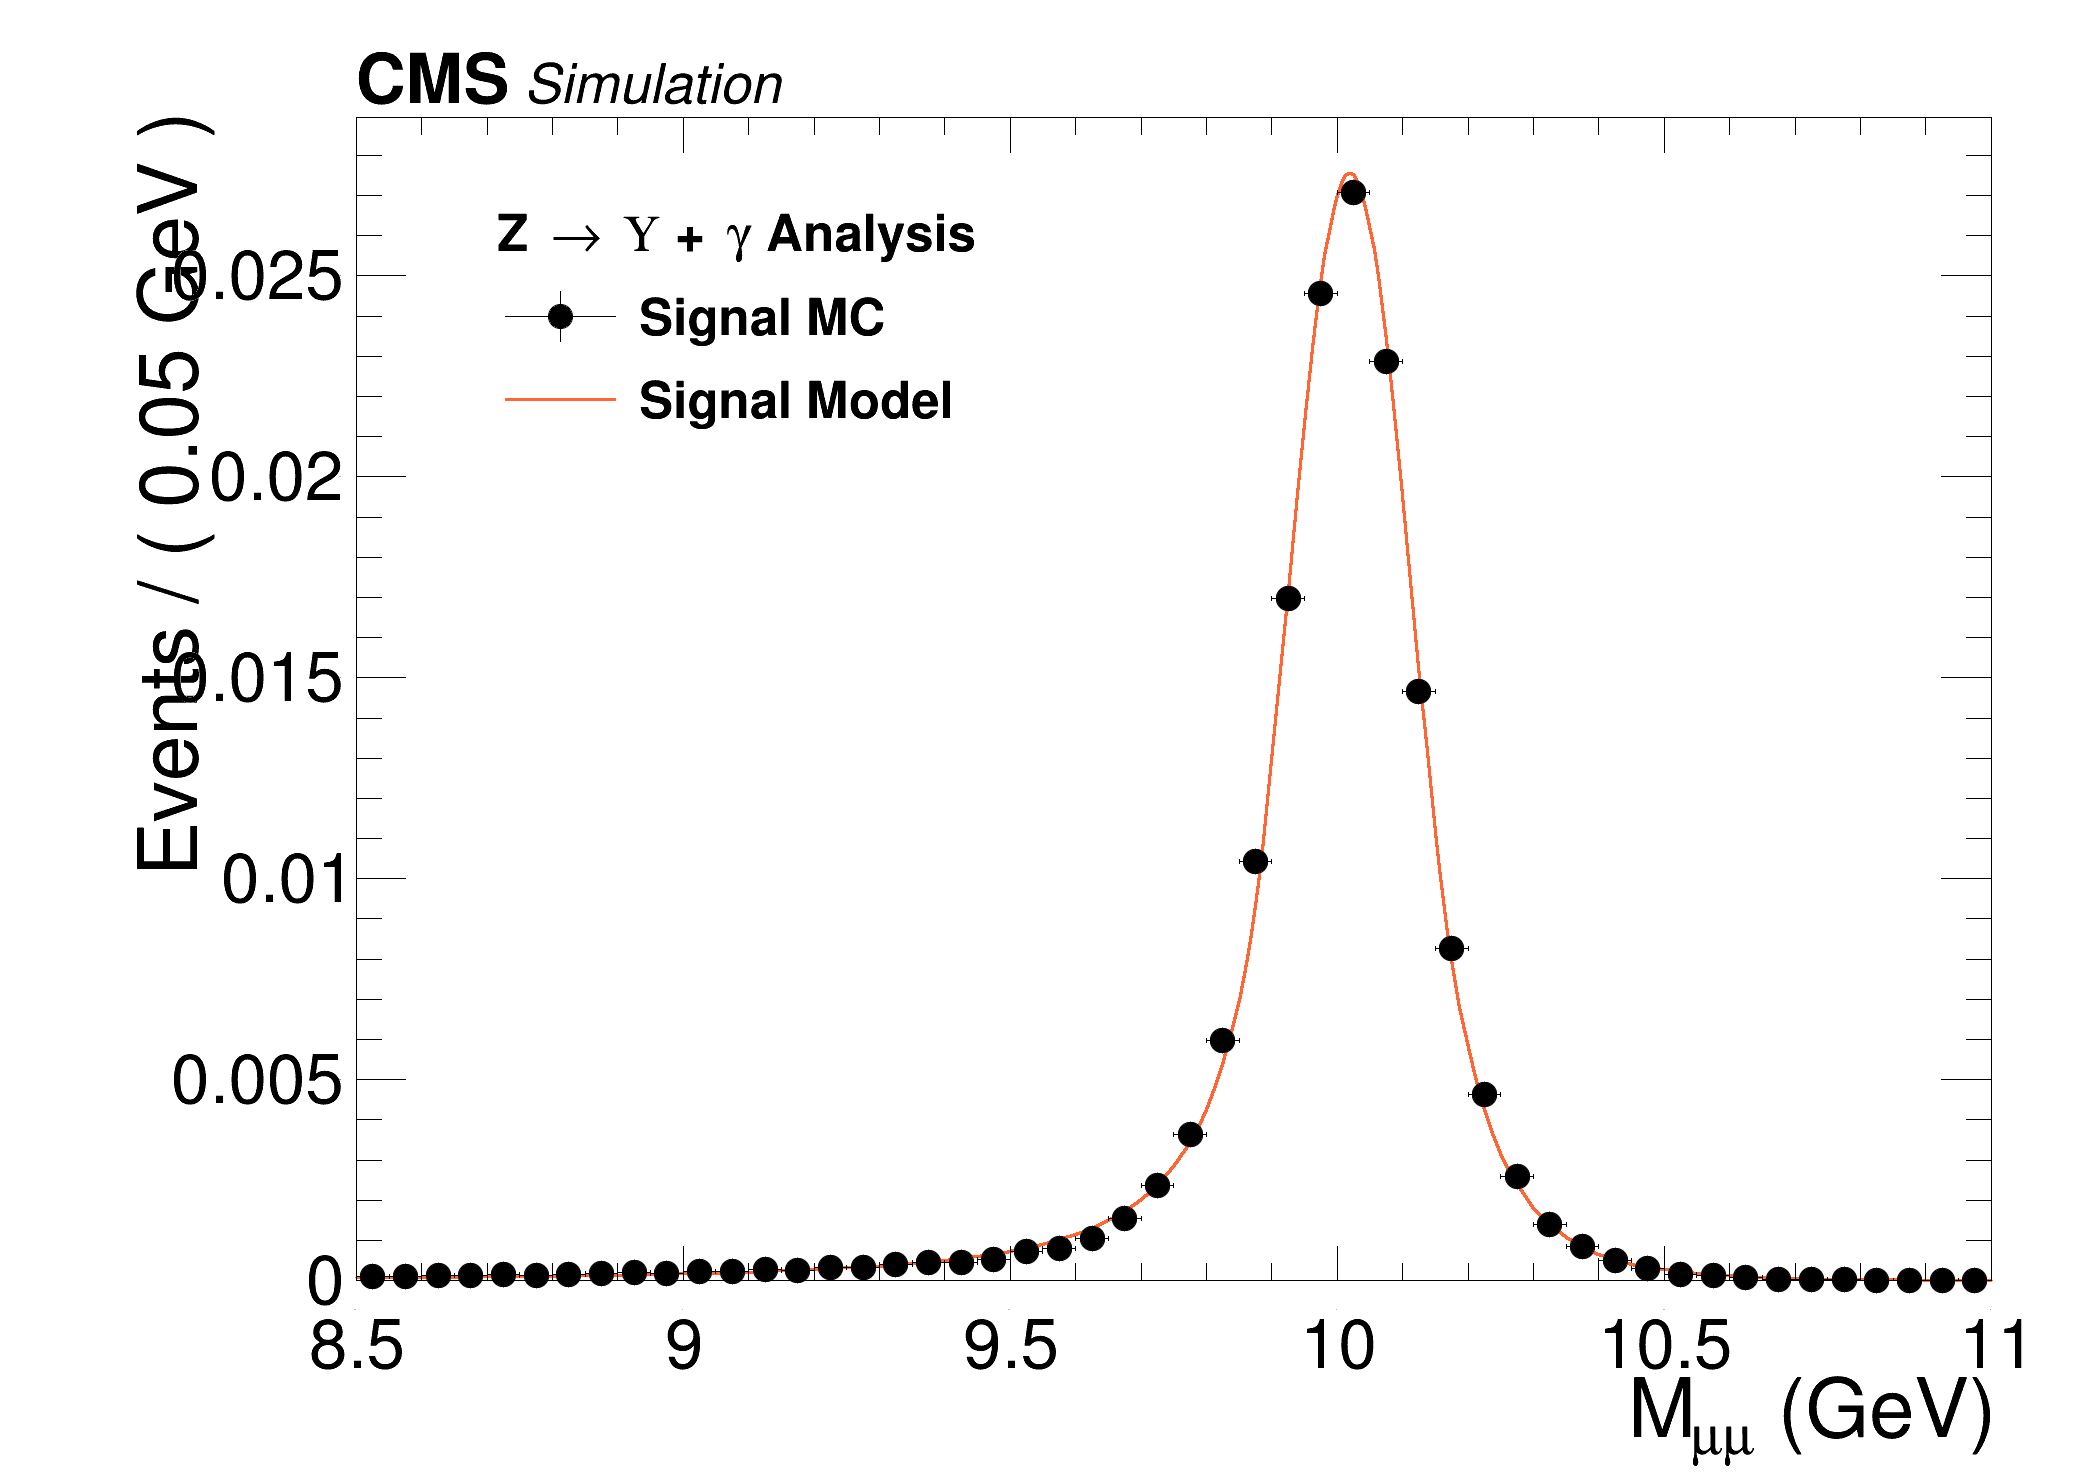
\includegraphics[width=0.45\textwidth]{figures_and_tables/fitPlotFiles2D/ZToUpsilonPhotonSignalAndBackgroundFit/mMuMNU_ZToUpsilon2SPhotonSignalAndBackgroundFit_Signal_Cat0}\hspace*{1.cm}
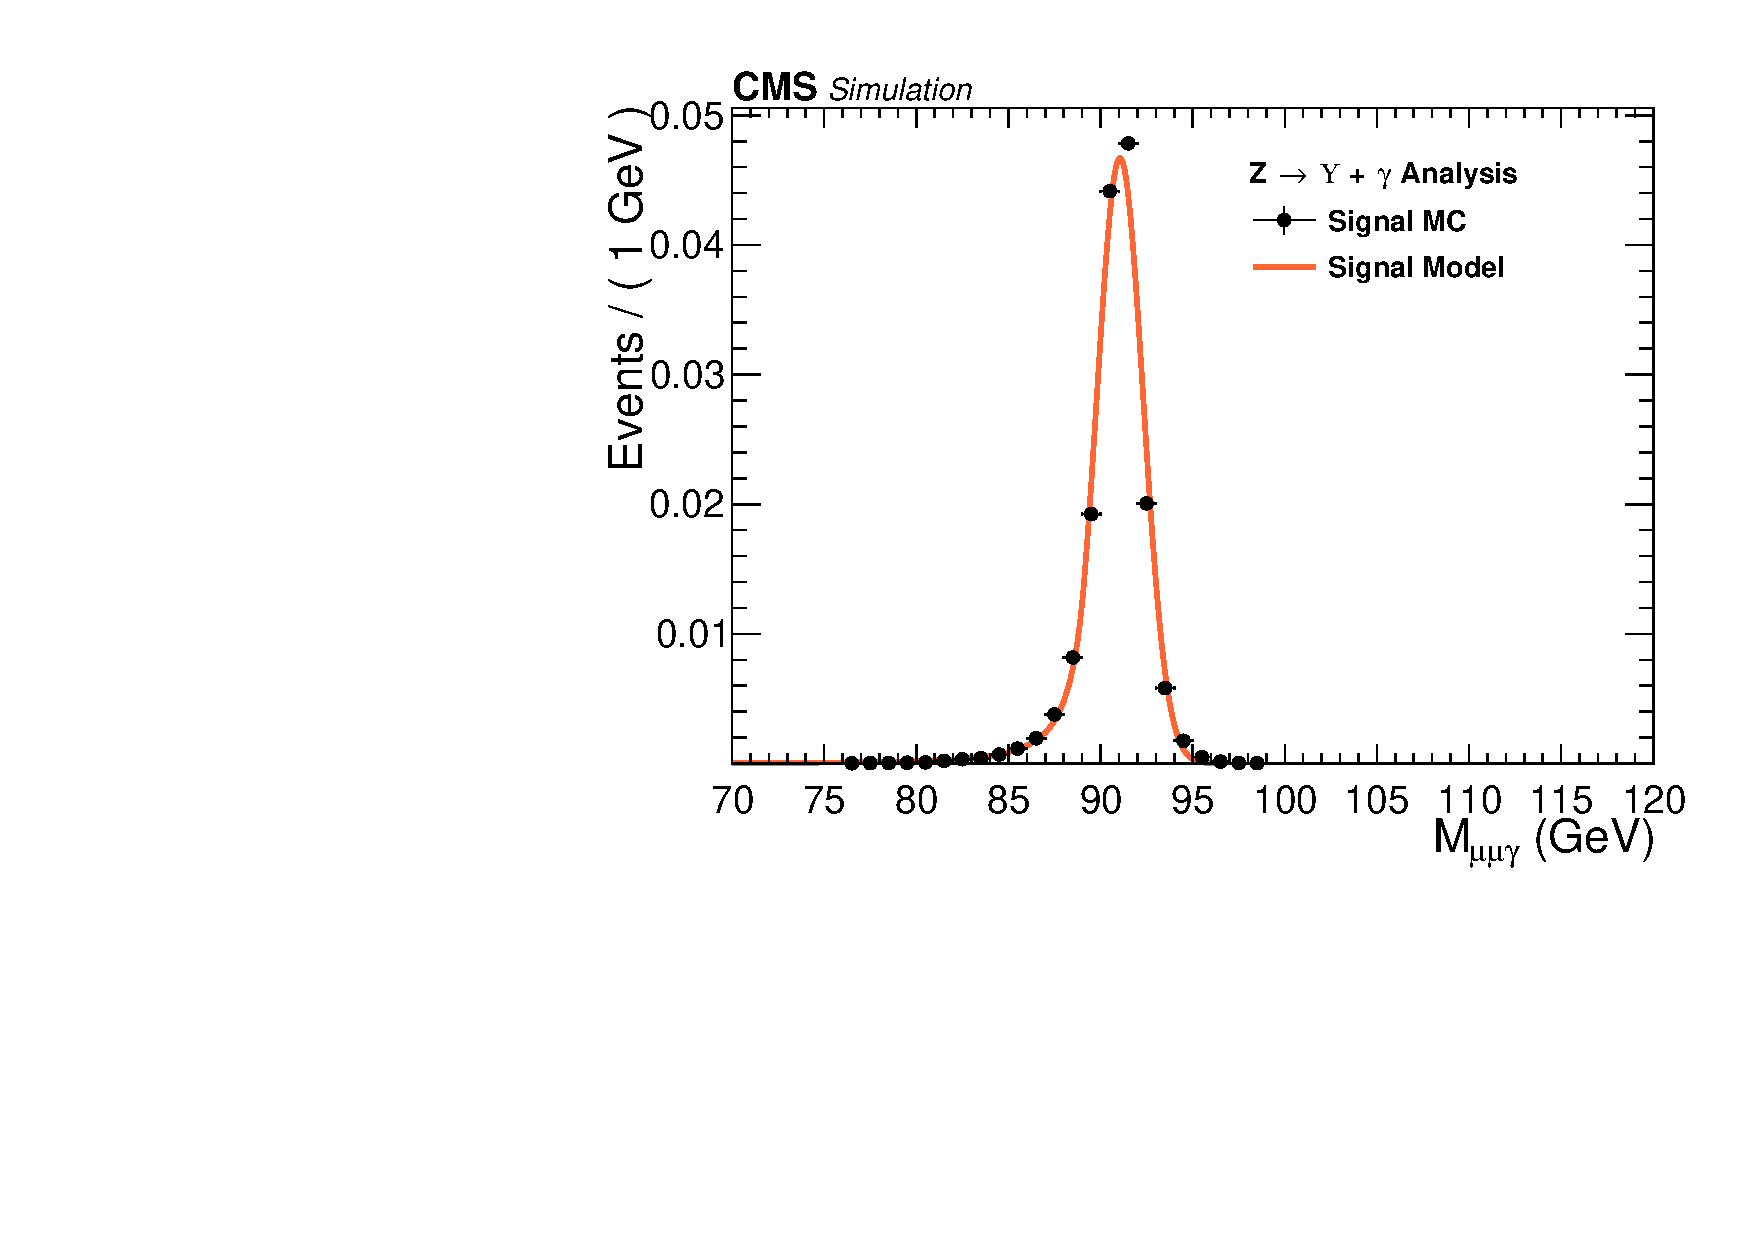
\includegraphics[width=0.45\textwidth]{figures_and_tables/fitPlotFiles2D/ZToUpsilonPhotonSignalAndBackgroundFit/mHZ_ZToUpsilon2SPhotonSignalAndBackgroundFit_Signal_Cat0_default}\hspace*{1.cm}

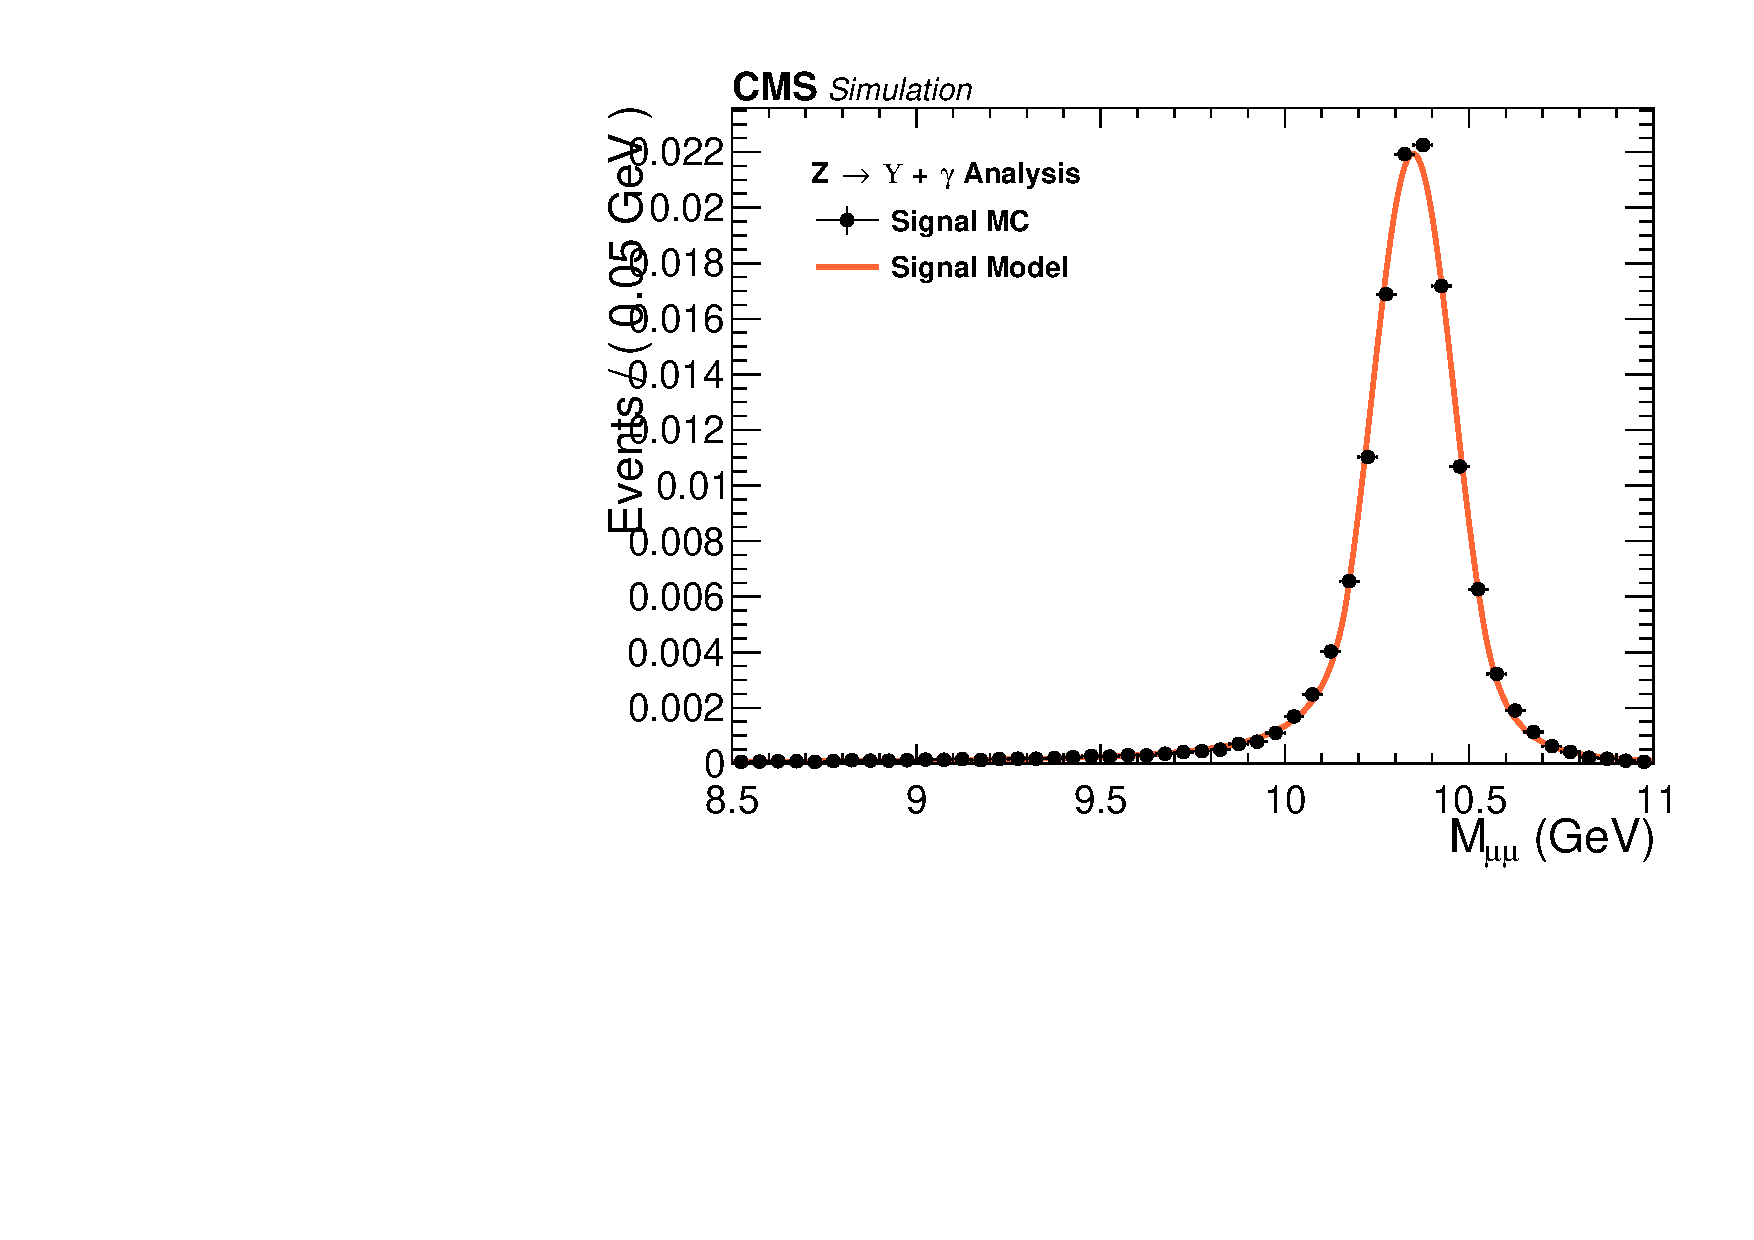
\includegraphics[width=0.45\textwidth]{figures_and_tables/fitPlotFiles2D/ZToUpsilonPhotonSignalAndBackgroundFit/mMuMNU_ZToUpsilon3SPhotonSignalAndBackgroundFit_Signal_Cat0}\hspace*{1.cm}
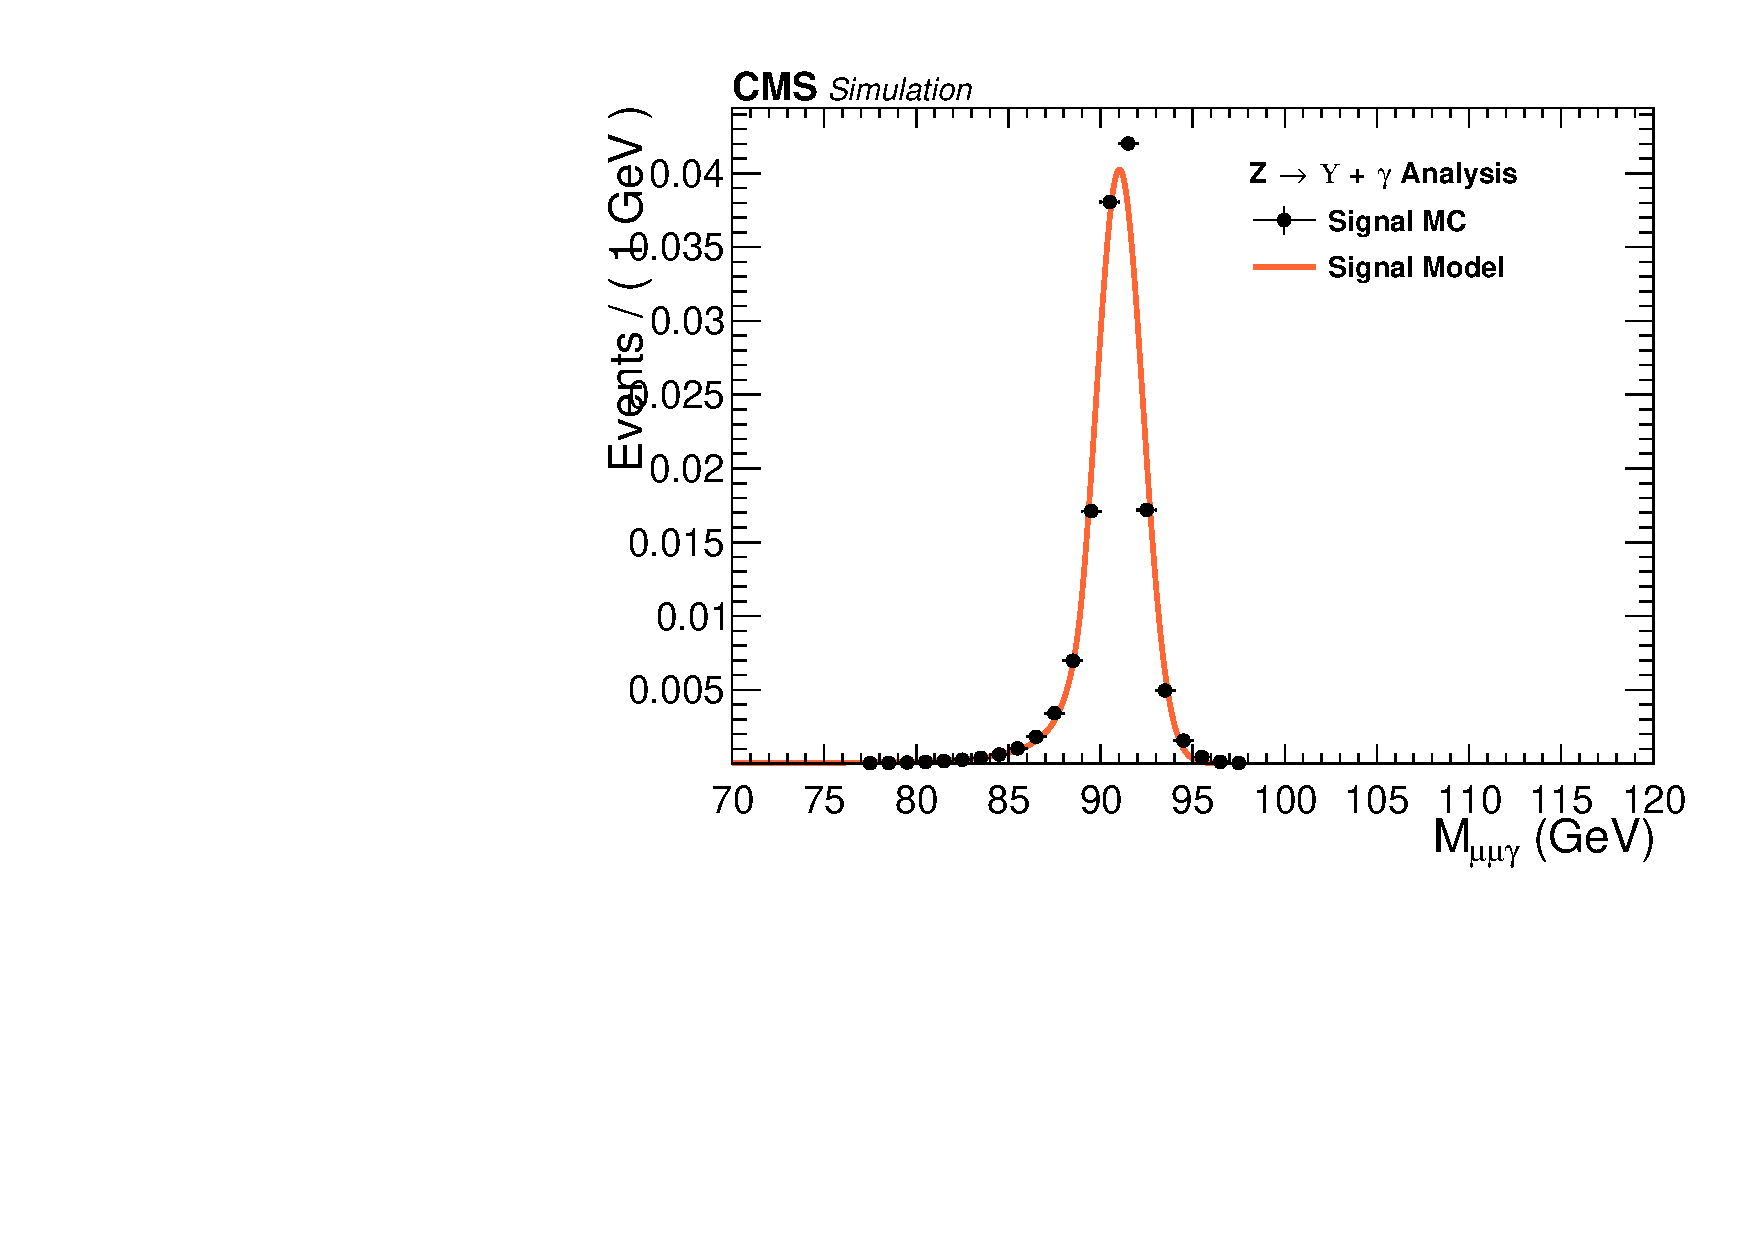
\includegraphics[width=0.45\textwidth]{figures_and_tables/fitPlotFiles2D/ZToUpsilonPhotonSignalAndBackgroundFit/mHZ_ZToUpsilon3SPhotonSignalAndBackgroundFit_Signal_Cat0_default}\hspace*{1.cm}


\end{center}\vspace*{-.5cm}
\caption{Signal Modeling for the $Z \rightarrow \Upsilon(1S,2S,3S) +\gamma$ analysis for Inclusive category. $m_{\mu\mu}$ mass distribution (left) and $m_{\mu\mu\gamma}$ mass distribution (right). From top to bottom: $\Upsilon(1S)$, $\Upsilon(2S)$, $\Upsilon(3S)$.}
\label{fig:ZToUpsilon_Signal_Cat0}
\end{figure}

% Cat1
\begin{figure}[!htbp]
\begin{center}


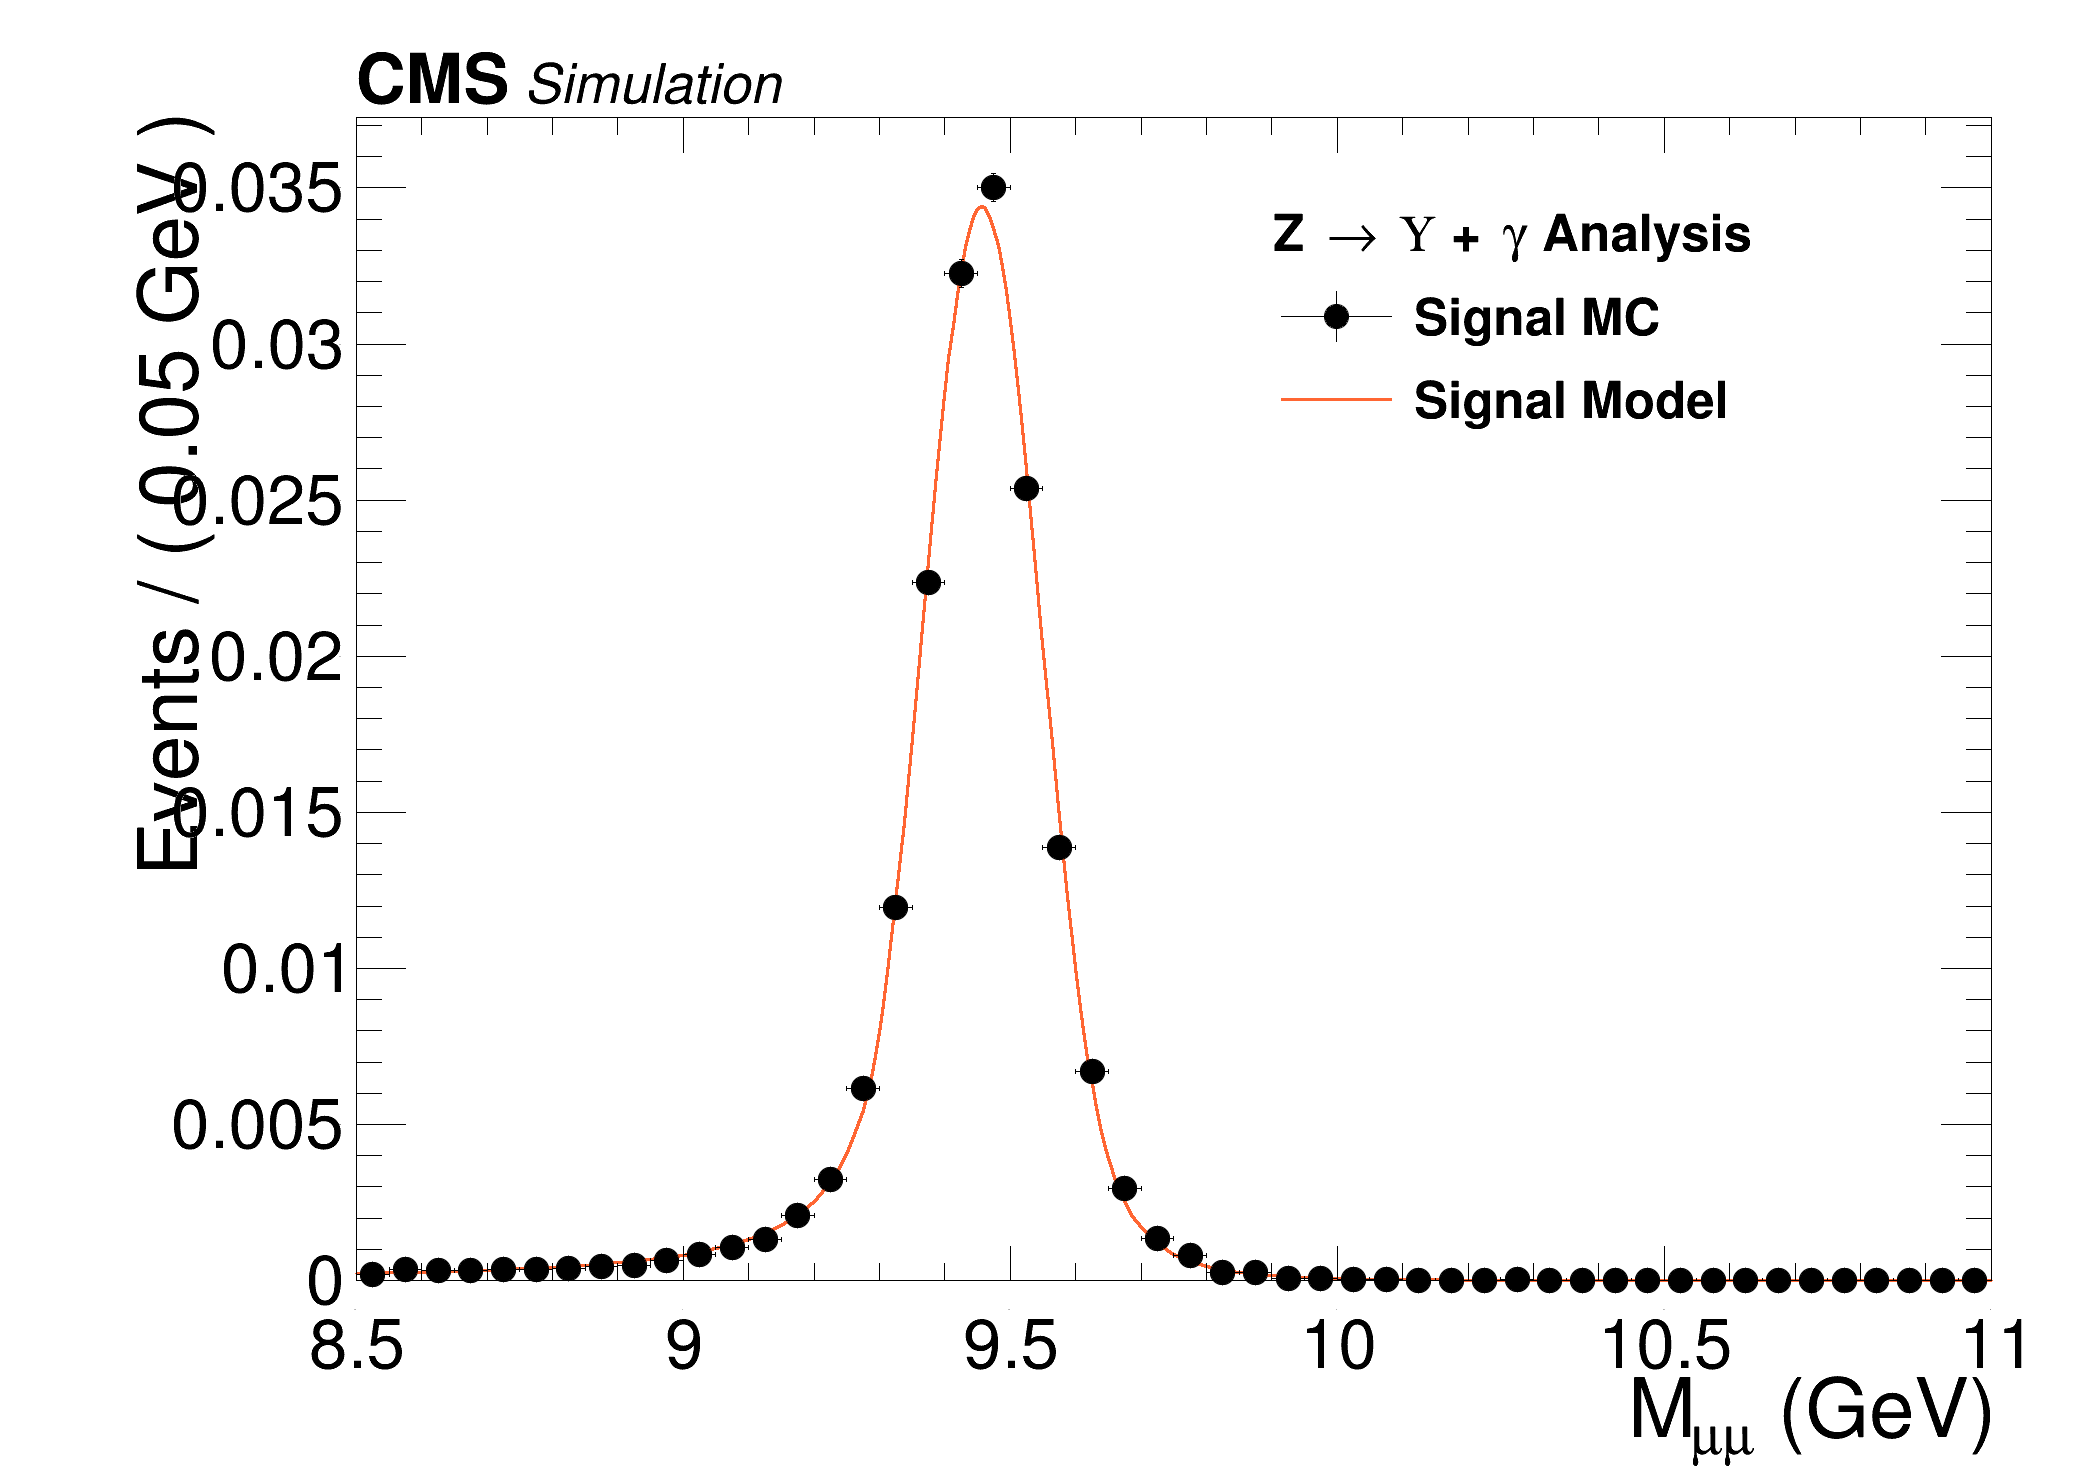
\includegraphics[width=0.45\textwidth]{figures_and_tables/fitPlotFiles2D/ZToUpsilonPhotonSignalAndBackgroundFit/mMuMNU_ZToUpsilon1SPhotonSignalAndBackgroundFit_Signal_Cat1}\hspace*{1.cm}
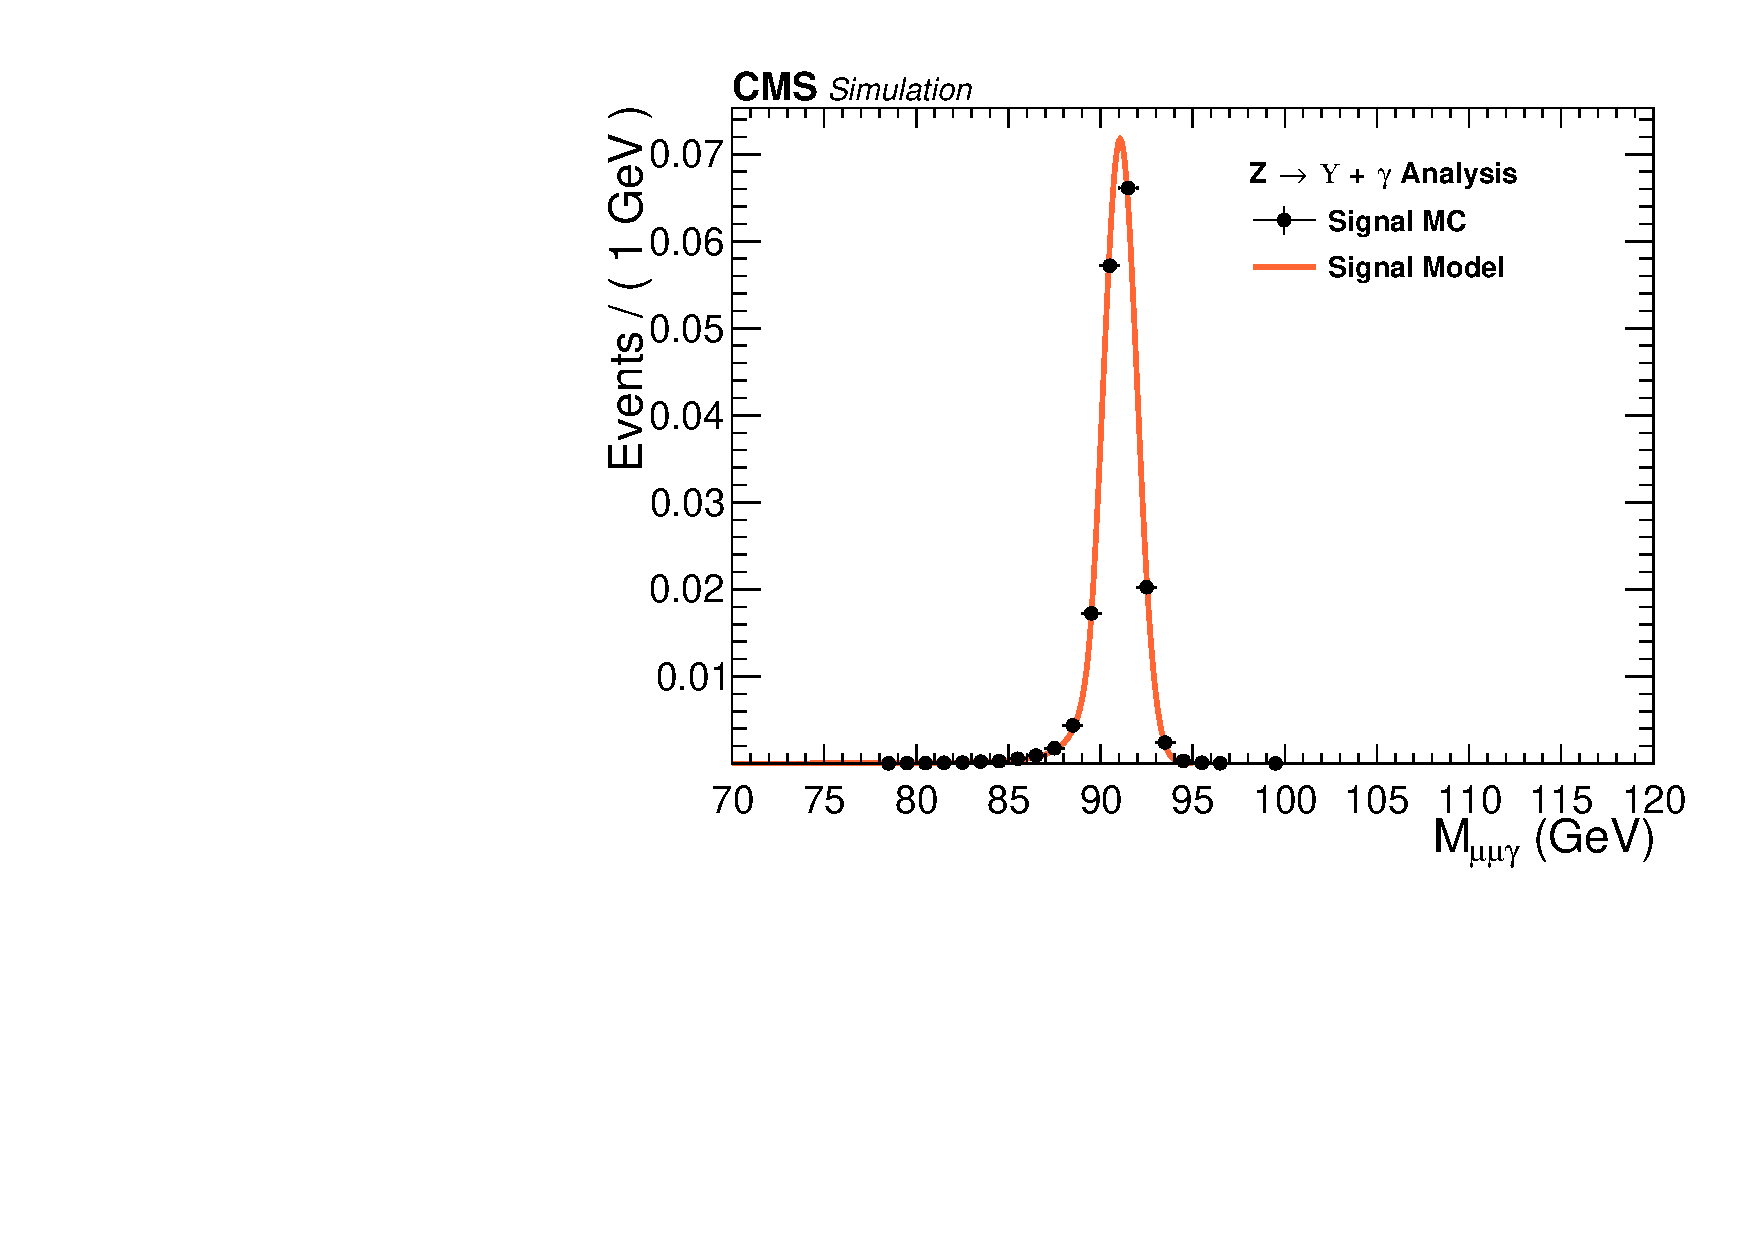
\includegraphics[width=0.45\textwidth]{figures_and_tables/fitPlotFiles2D/ZToUpsilonPhotonSignalAndBackgroundFit/mHZ_ZToUpsilon1SPhotonSignalAndBackgroundFit_Signal_Cat1_default}\hspace*{1.cm}

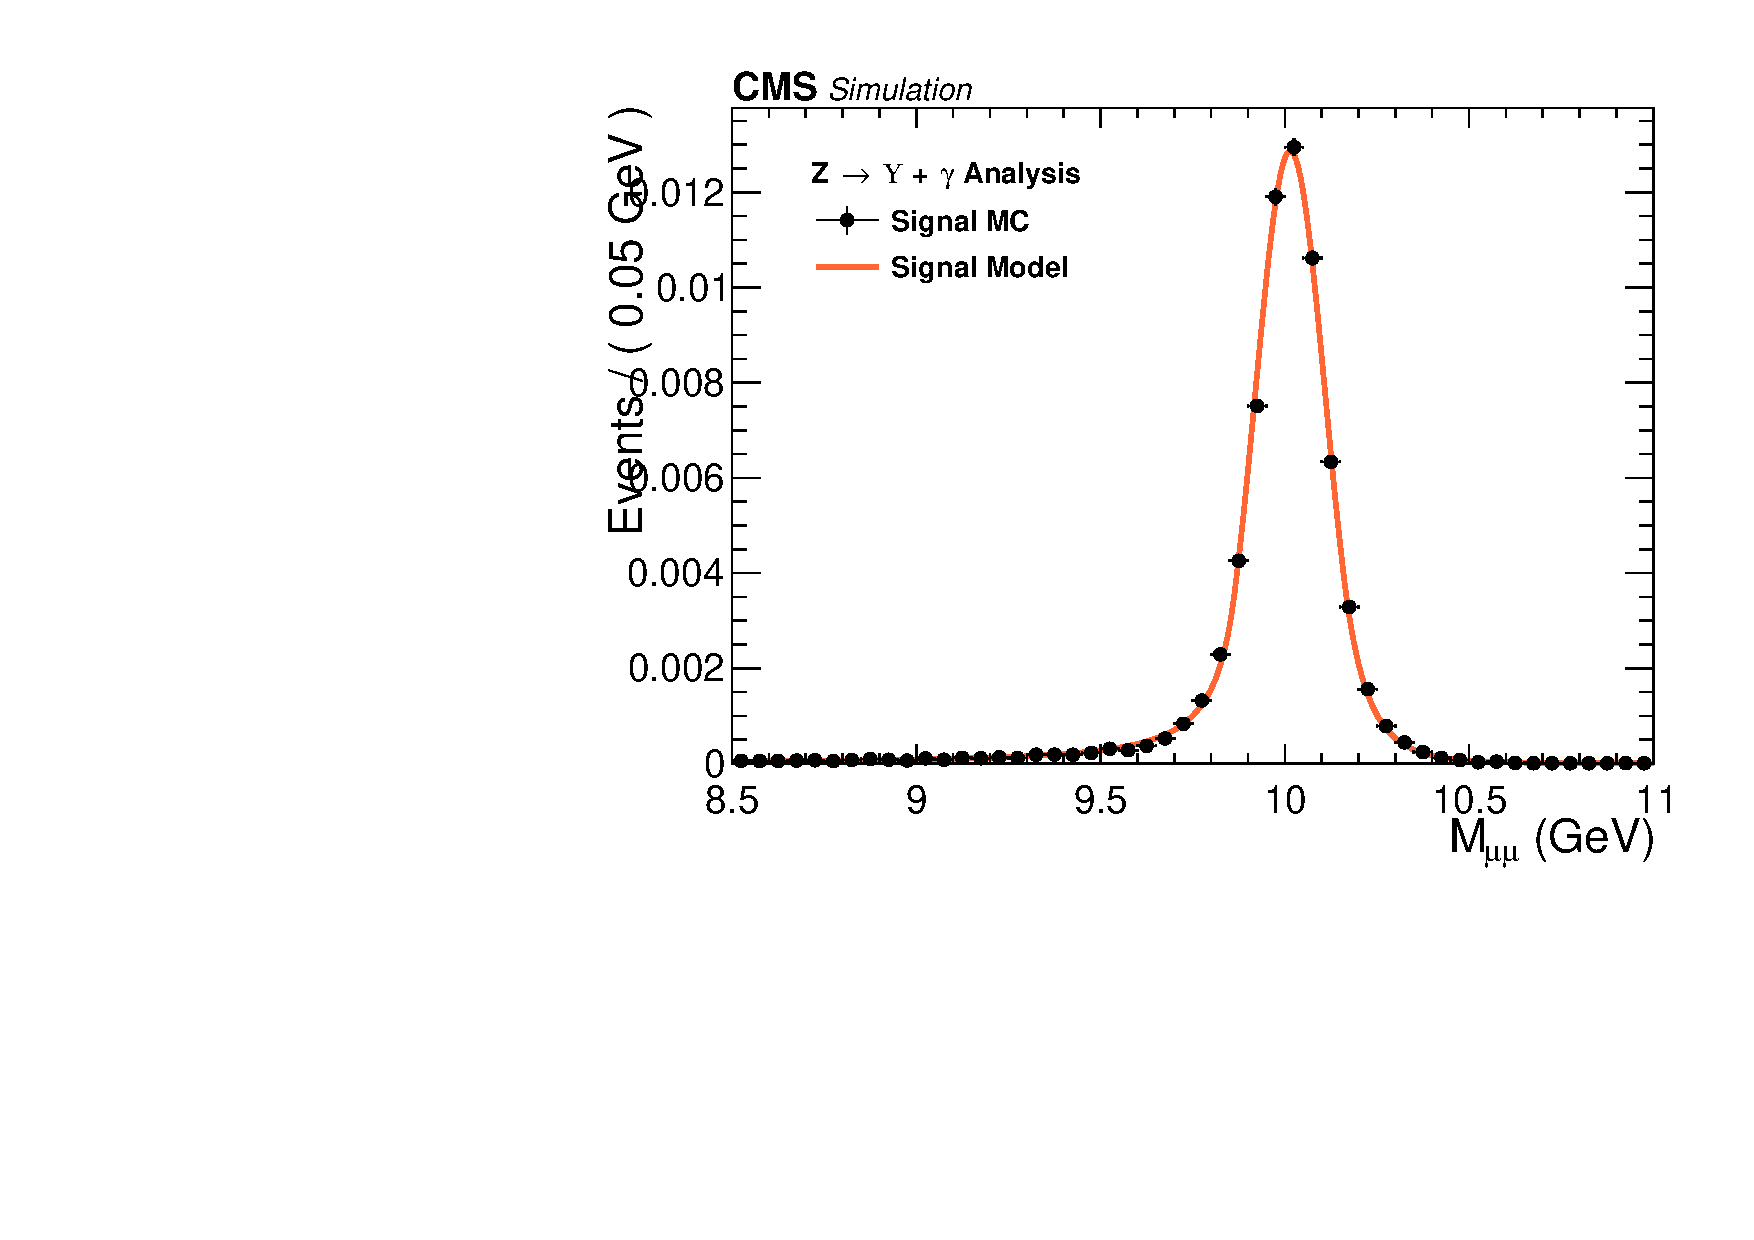
\includegraphics[width=0.45\textwidth]{figures_and_tables/fitPlotFiles2D/ZToUpsilonPhotonSignalAndBackgroundFit/mMuMNU_ZToUpsilon2SPhotonSignalAndBackgroundFit_Signal_Cat1}\hspace*{1.cm}
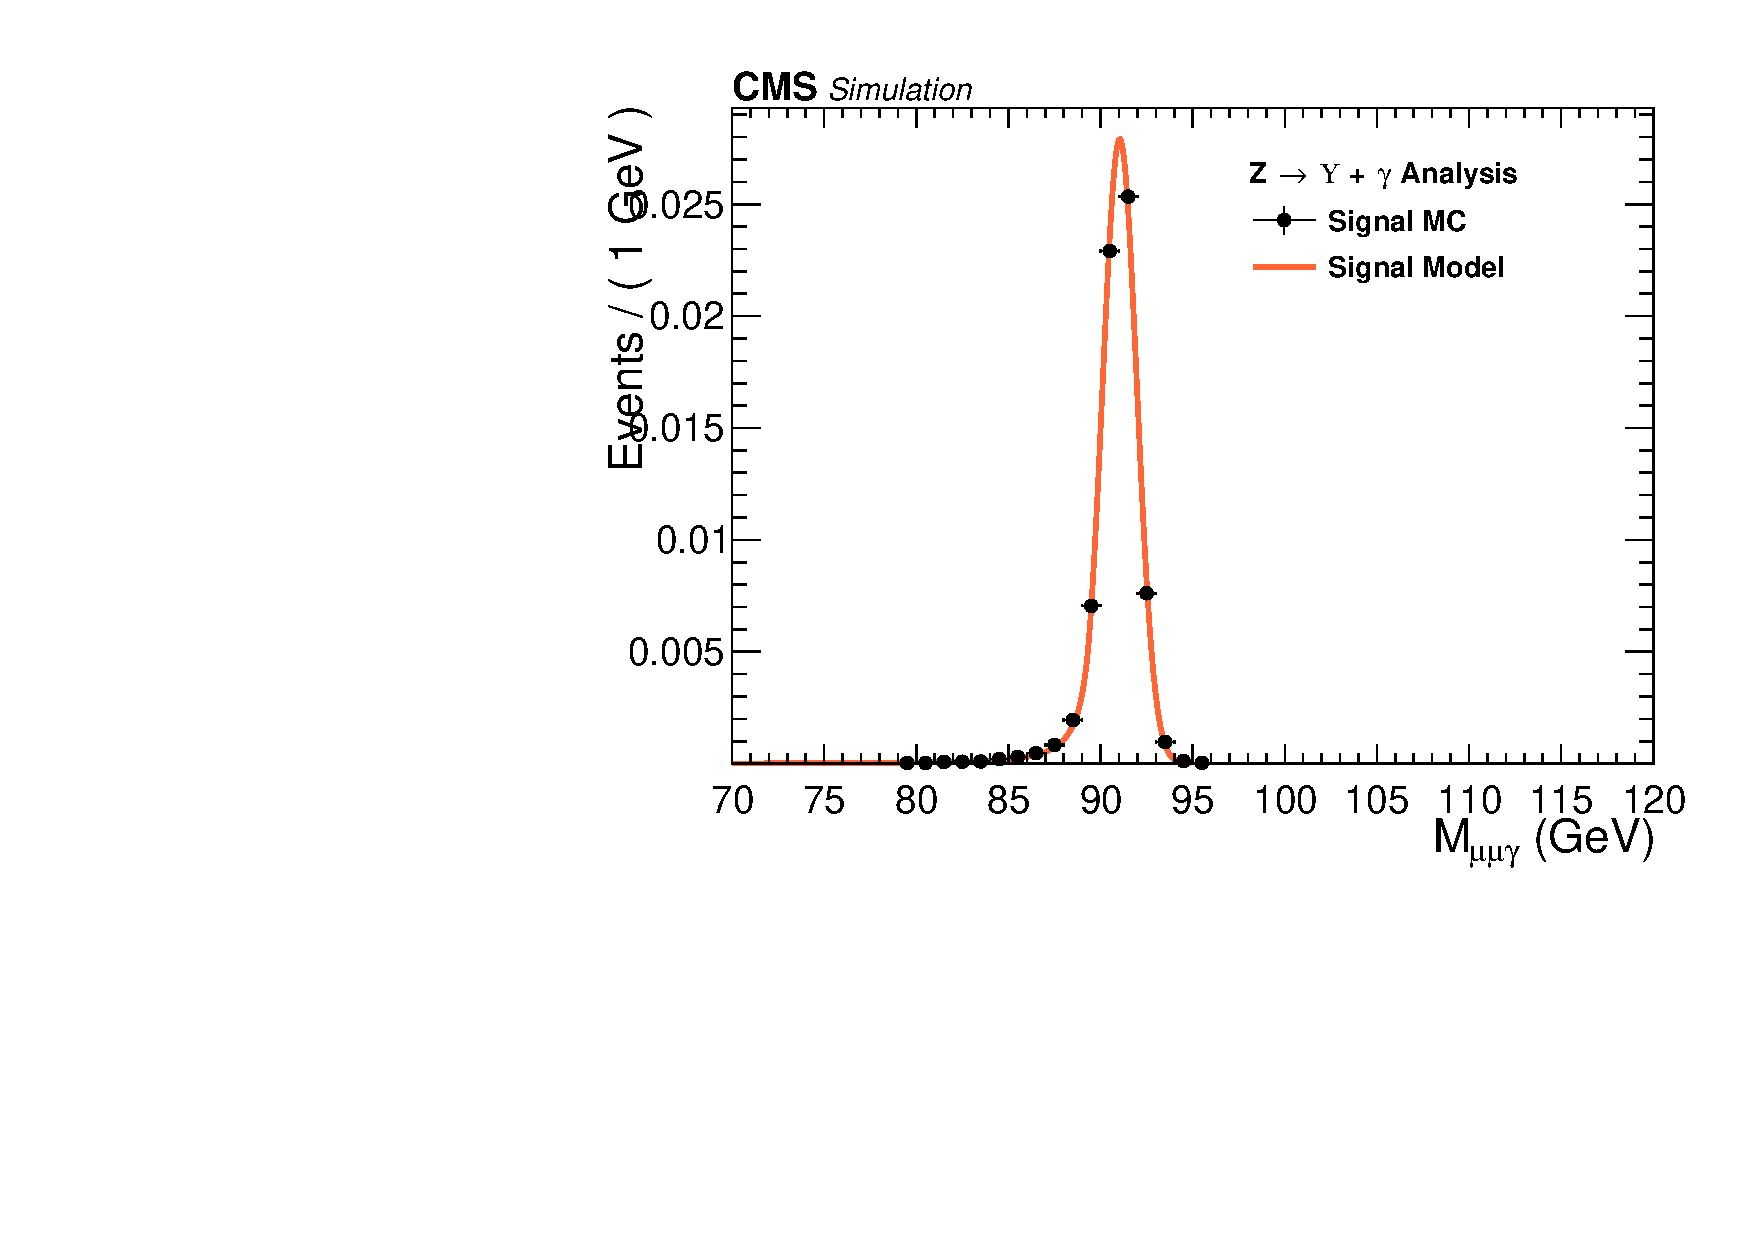
\includegraphics[width=0.45\textwidth]{figures_and_tables/fitPlotFiles2D/ZToUpsilonPhotonSignalAndBackgroundFit/mHZ_ZToUpsilon2SPhotonSignalAndBackgroundFit_Signal_Cat1_default}\hspace*{1.cm}

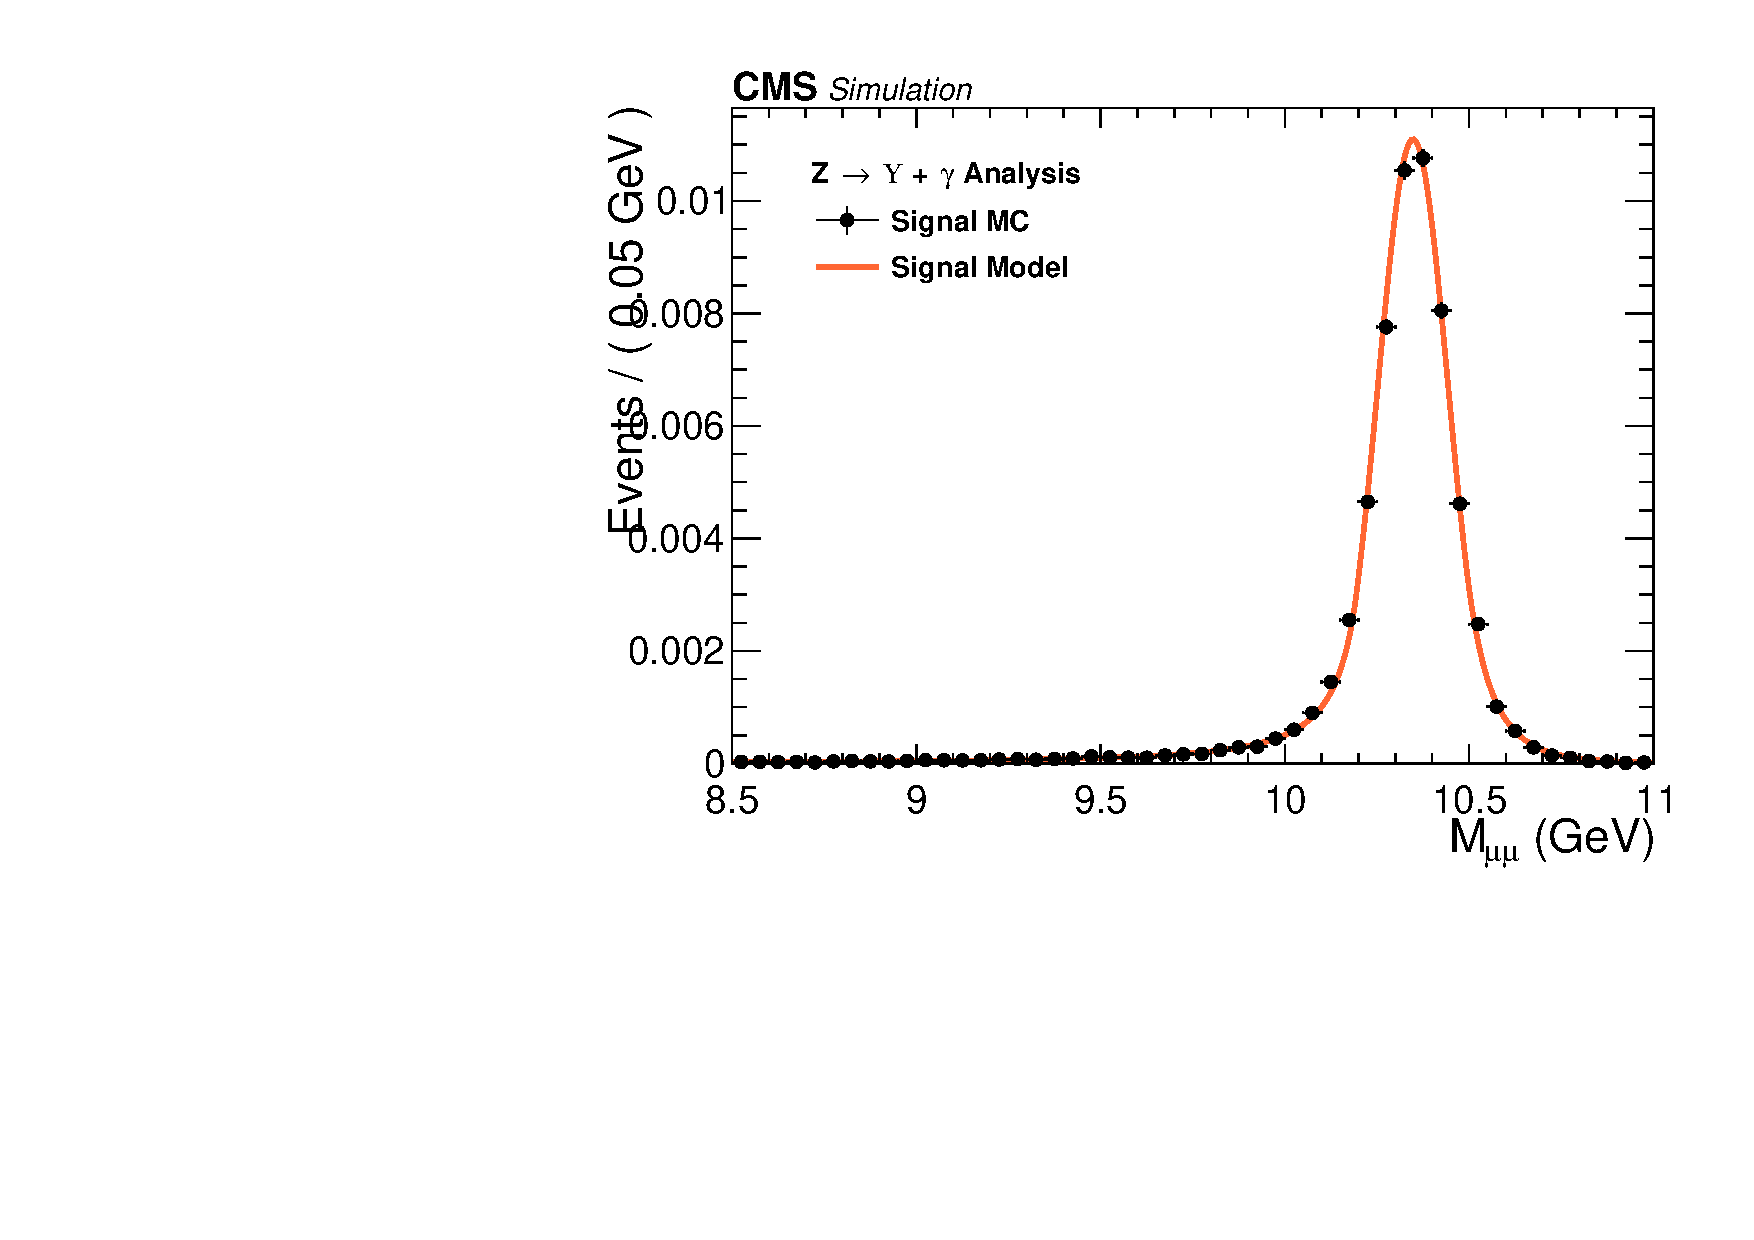
\includegraphics[width=0.45\textwidth]{figures_and_tables/fitPlotFiles2D/ZToUpsilonPhotonSignalAndBackgroundFit/mMuMNU_ZToUpsilon3SPhotonSignalAndBackgroundFit_Signal_Cat1}\hspace*{1.cm}
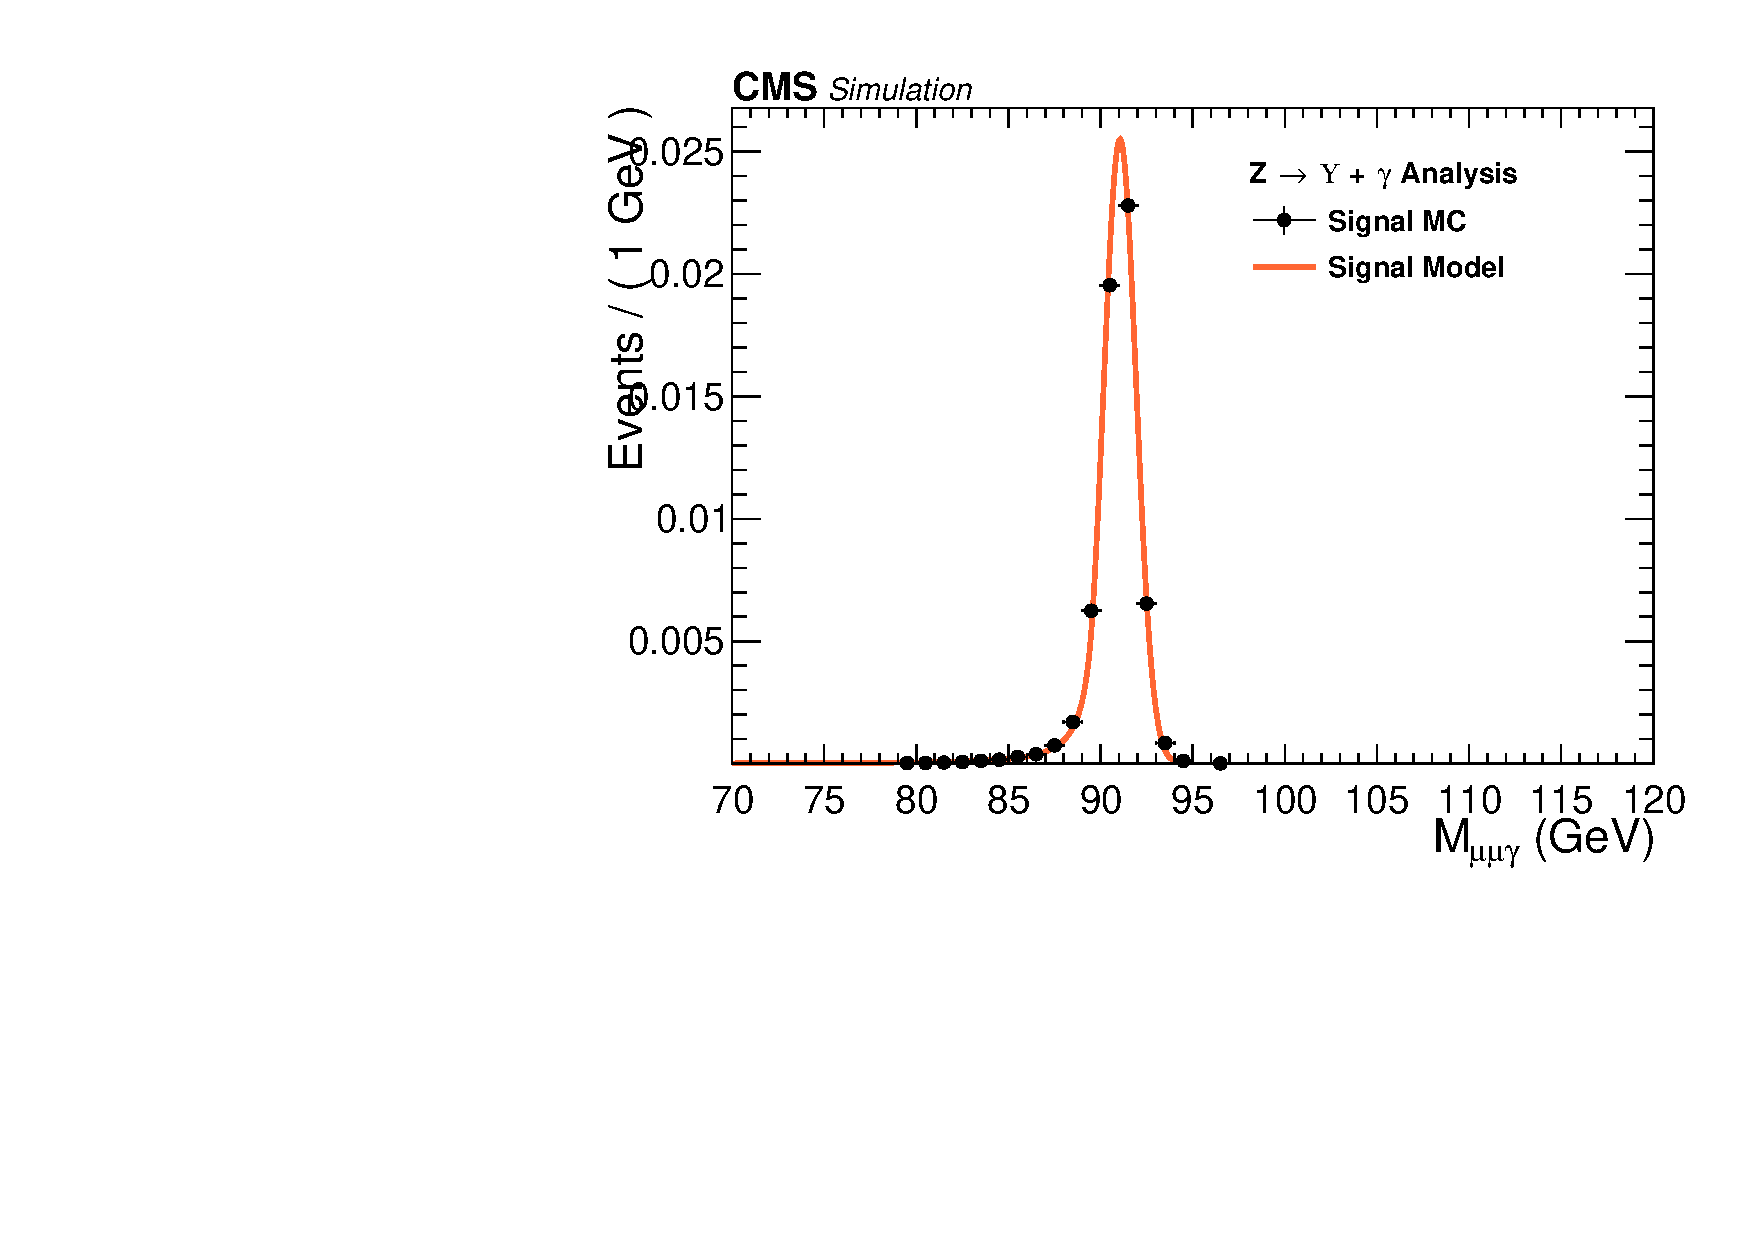
\includegraphics[width=0.45\textwidth]{figures_and_tables/fitPlotFiles2D/ZToUpsilonPhotonSignalAndBackgroundFit/mHZ_ZToUpsilon3SPhotonSignalAndBackgroundFit_Signal_Cat1_default}\hspace*{1.cm}


\end{center}\vspace*{-.5cm}
\caption{Signal Modeling for the $Z \rightarrow \Upsilon(1S,2S,3S) +\gamma$ analysis for EB High R9 category. $m_{\mu\mu}$ mass distribution (left) and $m_{\mu\mu\gamma}$ mass distribution (right). From top to bottom: $\Upsilon(1S)$, $\Upsilon(2S)$, $\Upsilon(3S)$.}
\label{fig:ZToUpsilon_Signal_Cat1}
\end{figure}

% Cat2
\begin{figure}[!htbp]
\begin{center}


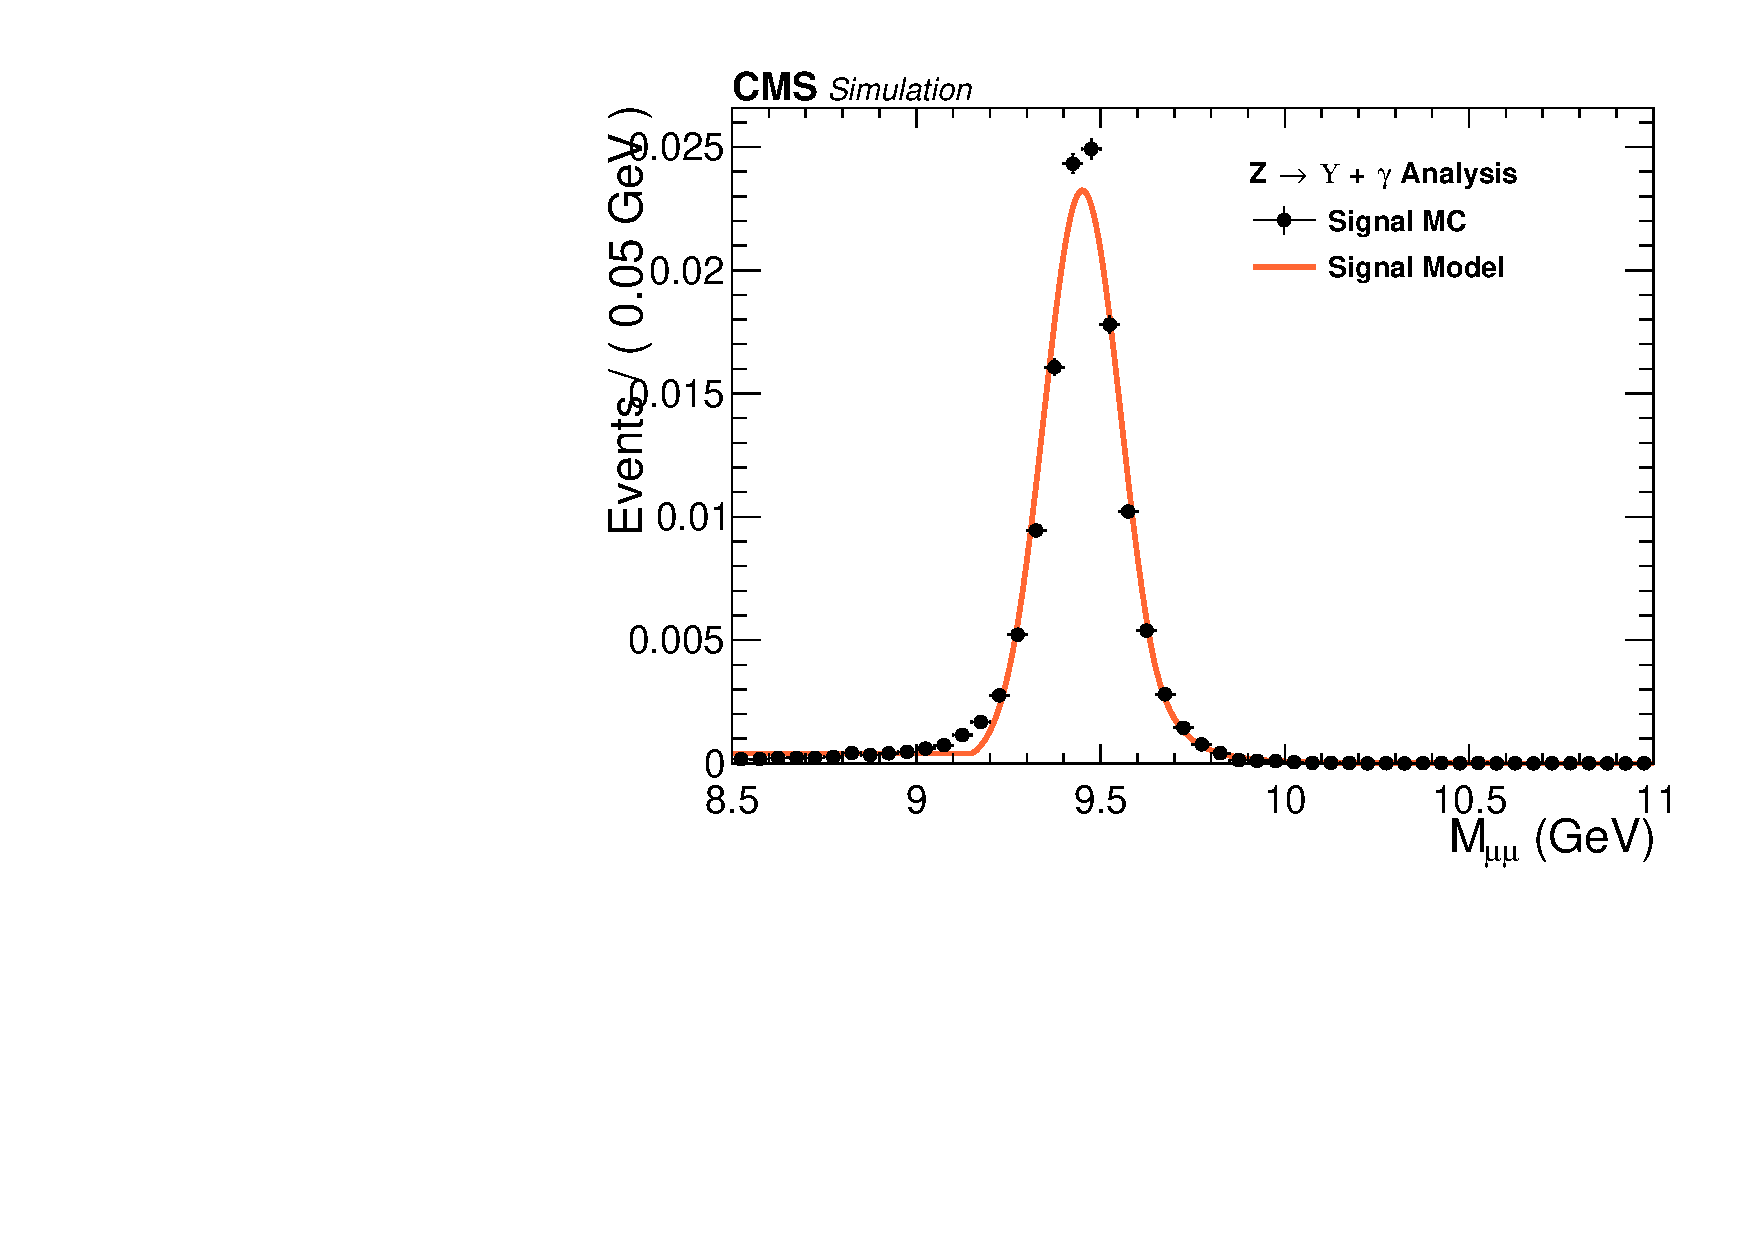
\includegraphics[width=0.45\textwidth]{figures_and_tables/fitPlotFiles2D/ZToUpsilonPhotonSignalAndBackgroundFit/mMuMNU_ZToUpsilon1SPhotonSignalAndBackgroundFit_Signal_Cat2}\hspace*{1.cm}
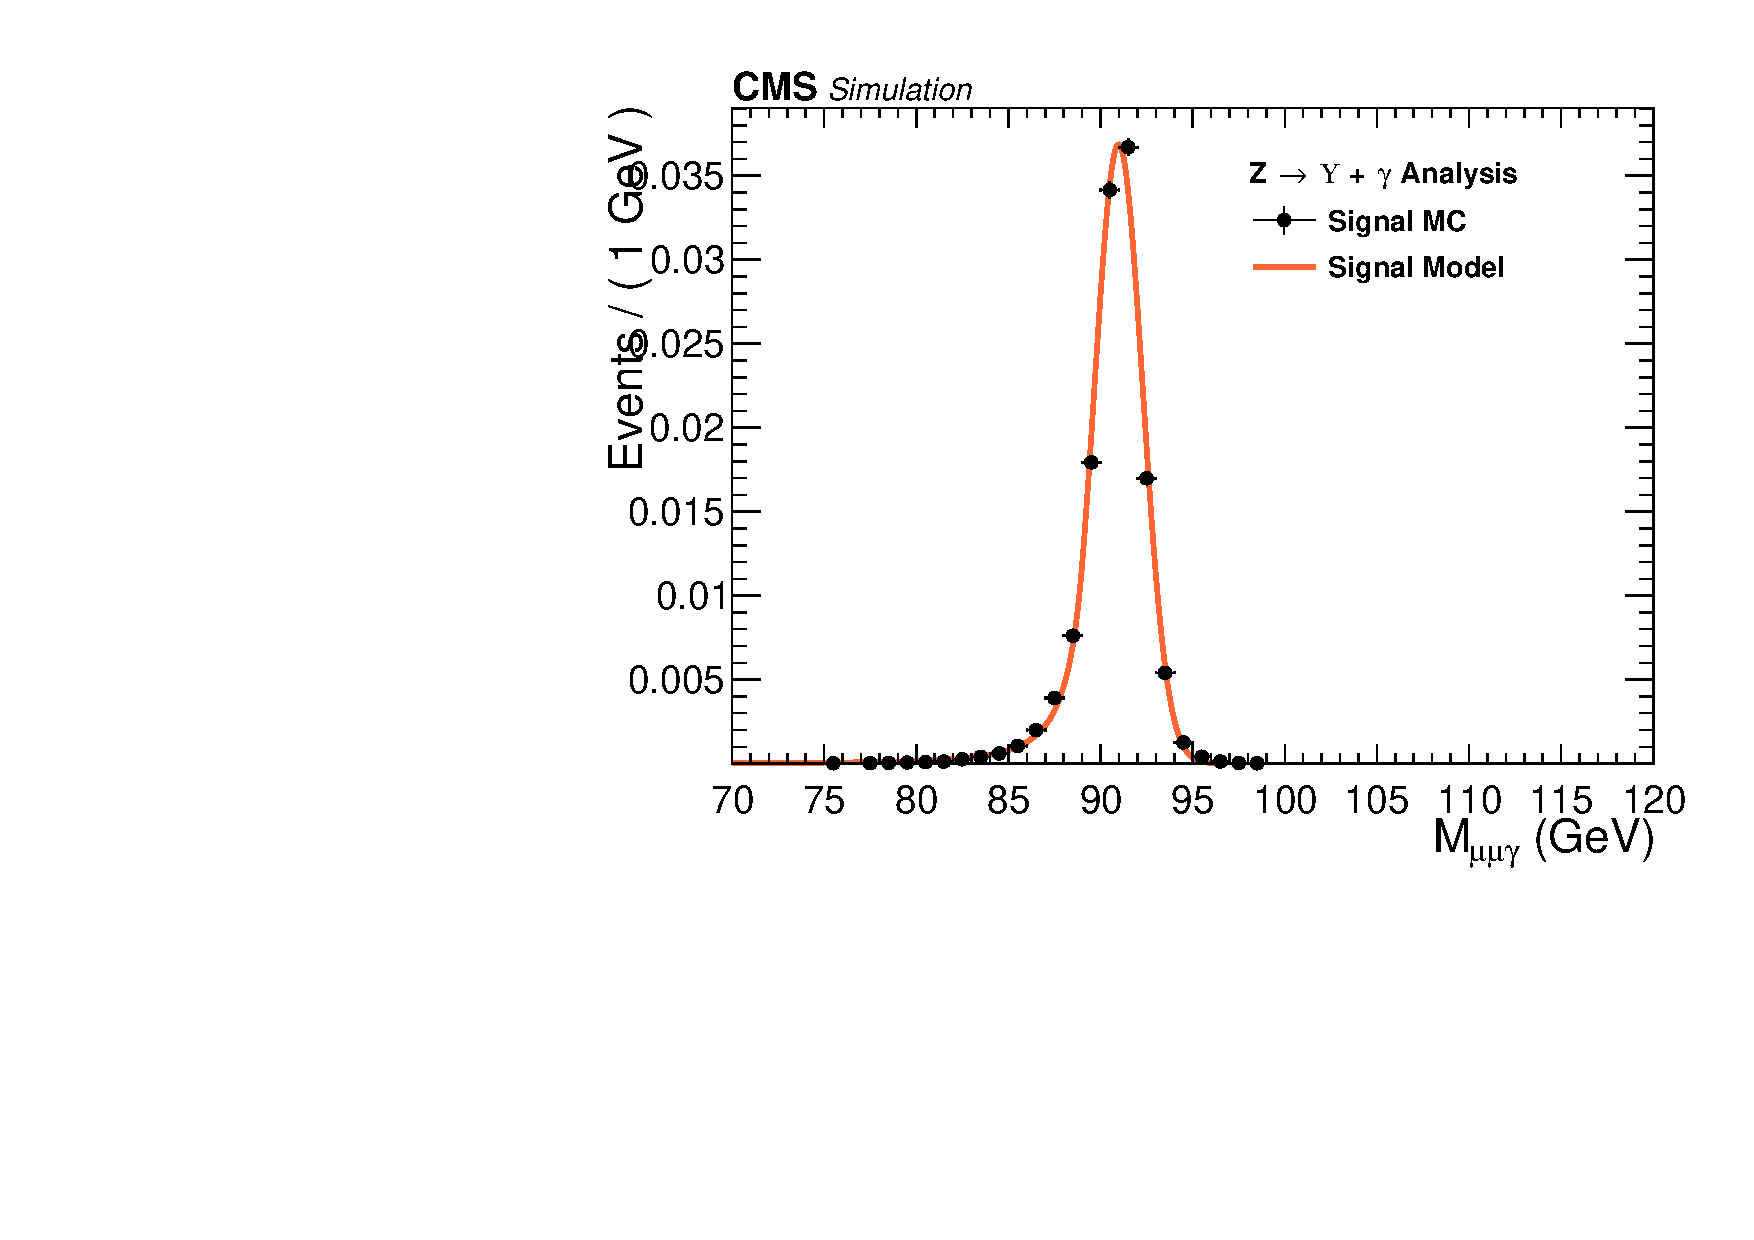
\includegraphics[width=0.45\textwidth]{figures_and_tables/fitPlotFiles2D/ZToUpsilonPhotonSignalAndBackgroundFit/mHZ_ZToUpsilon1SPhotonSignalAndBackgroundFit_Signal_Cat2_default}\hspace*{1.cm}

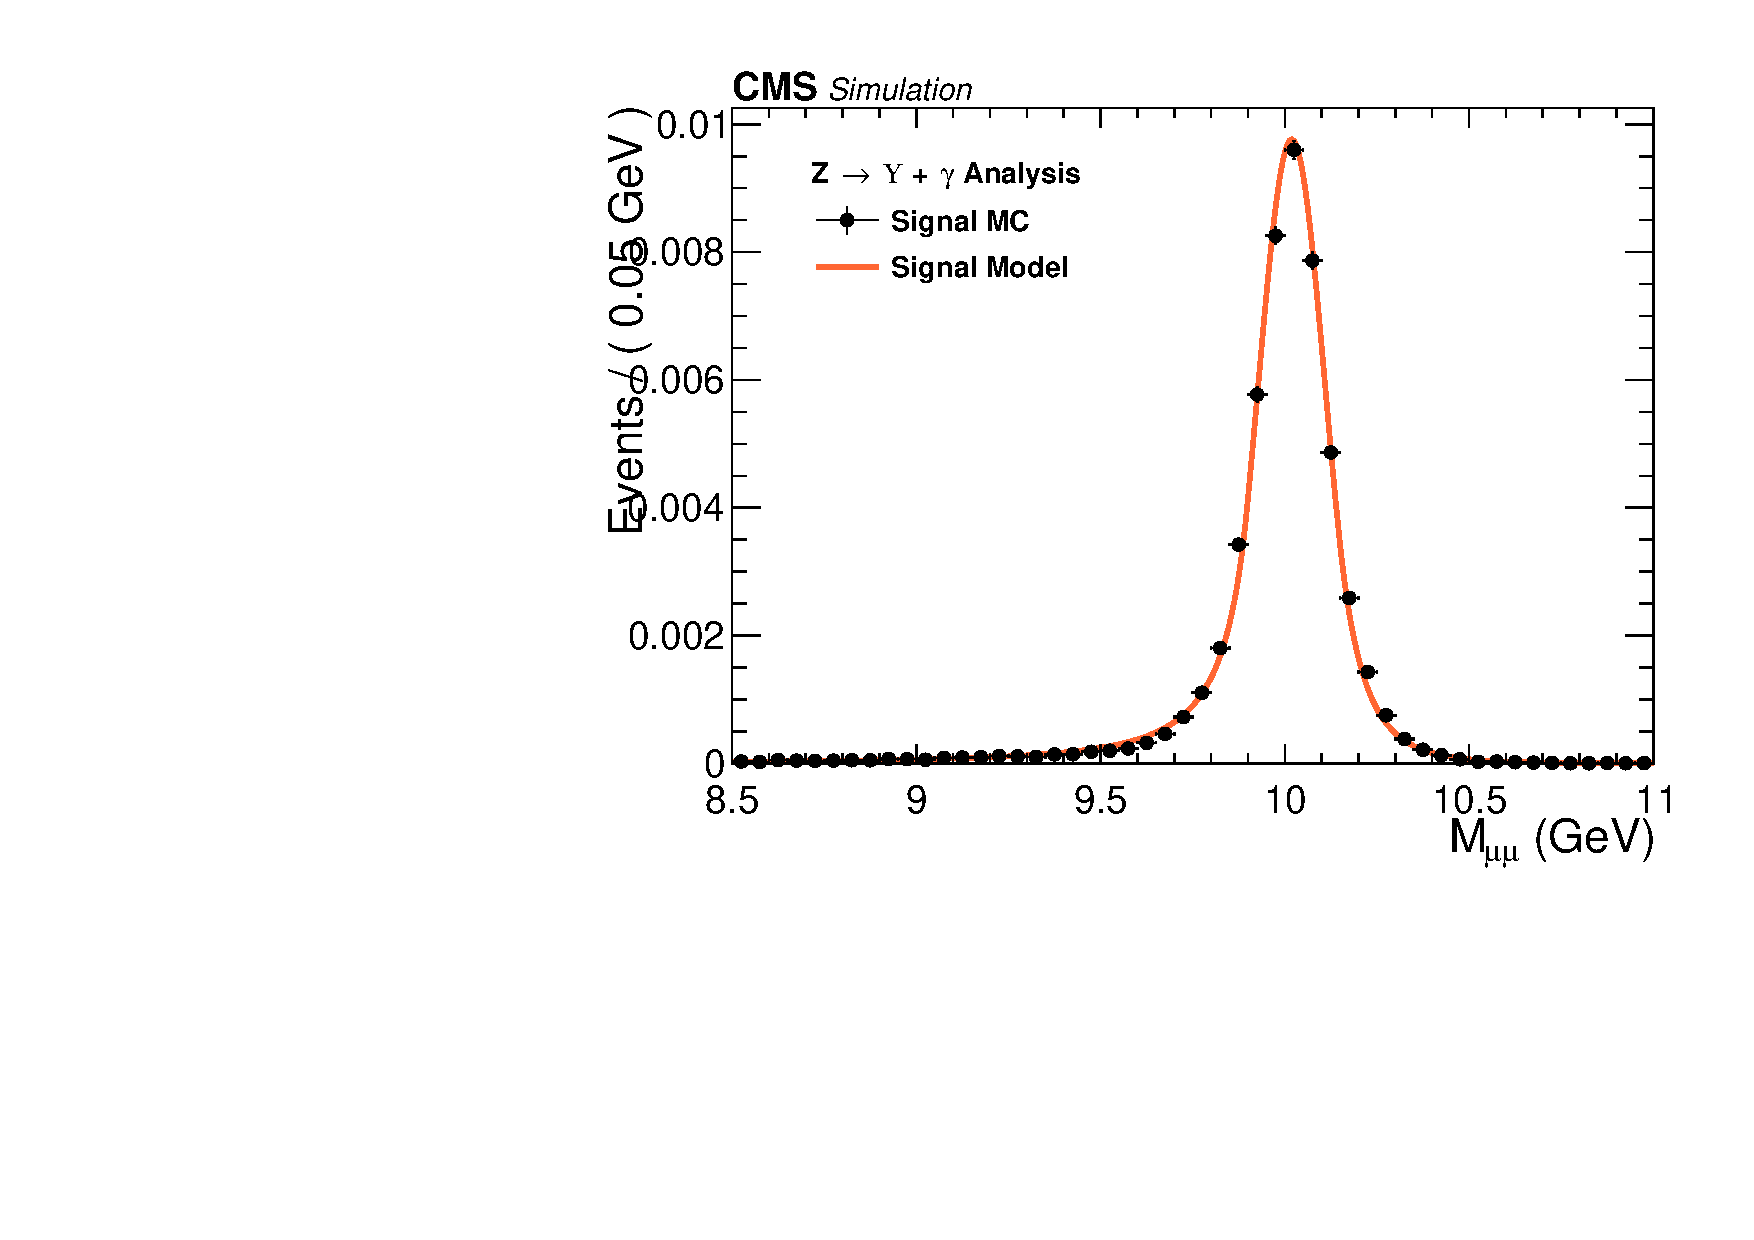
\includegraphics[width=0.45\textwidth]{figures_and_tables/fitPlotFiles2D/ZToUpsilonPhotonSignalAndBackgroundFit/mMuMNU_ZToUpsilon2SPhotonSignalAndBackgroundFit_Signal_Cat2}\hspace*{1.cm}
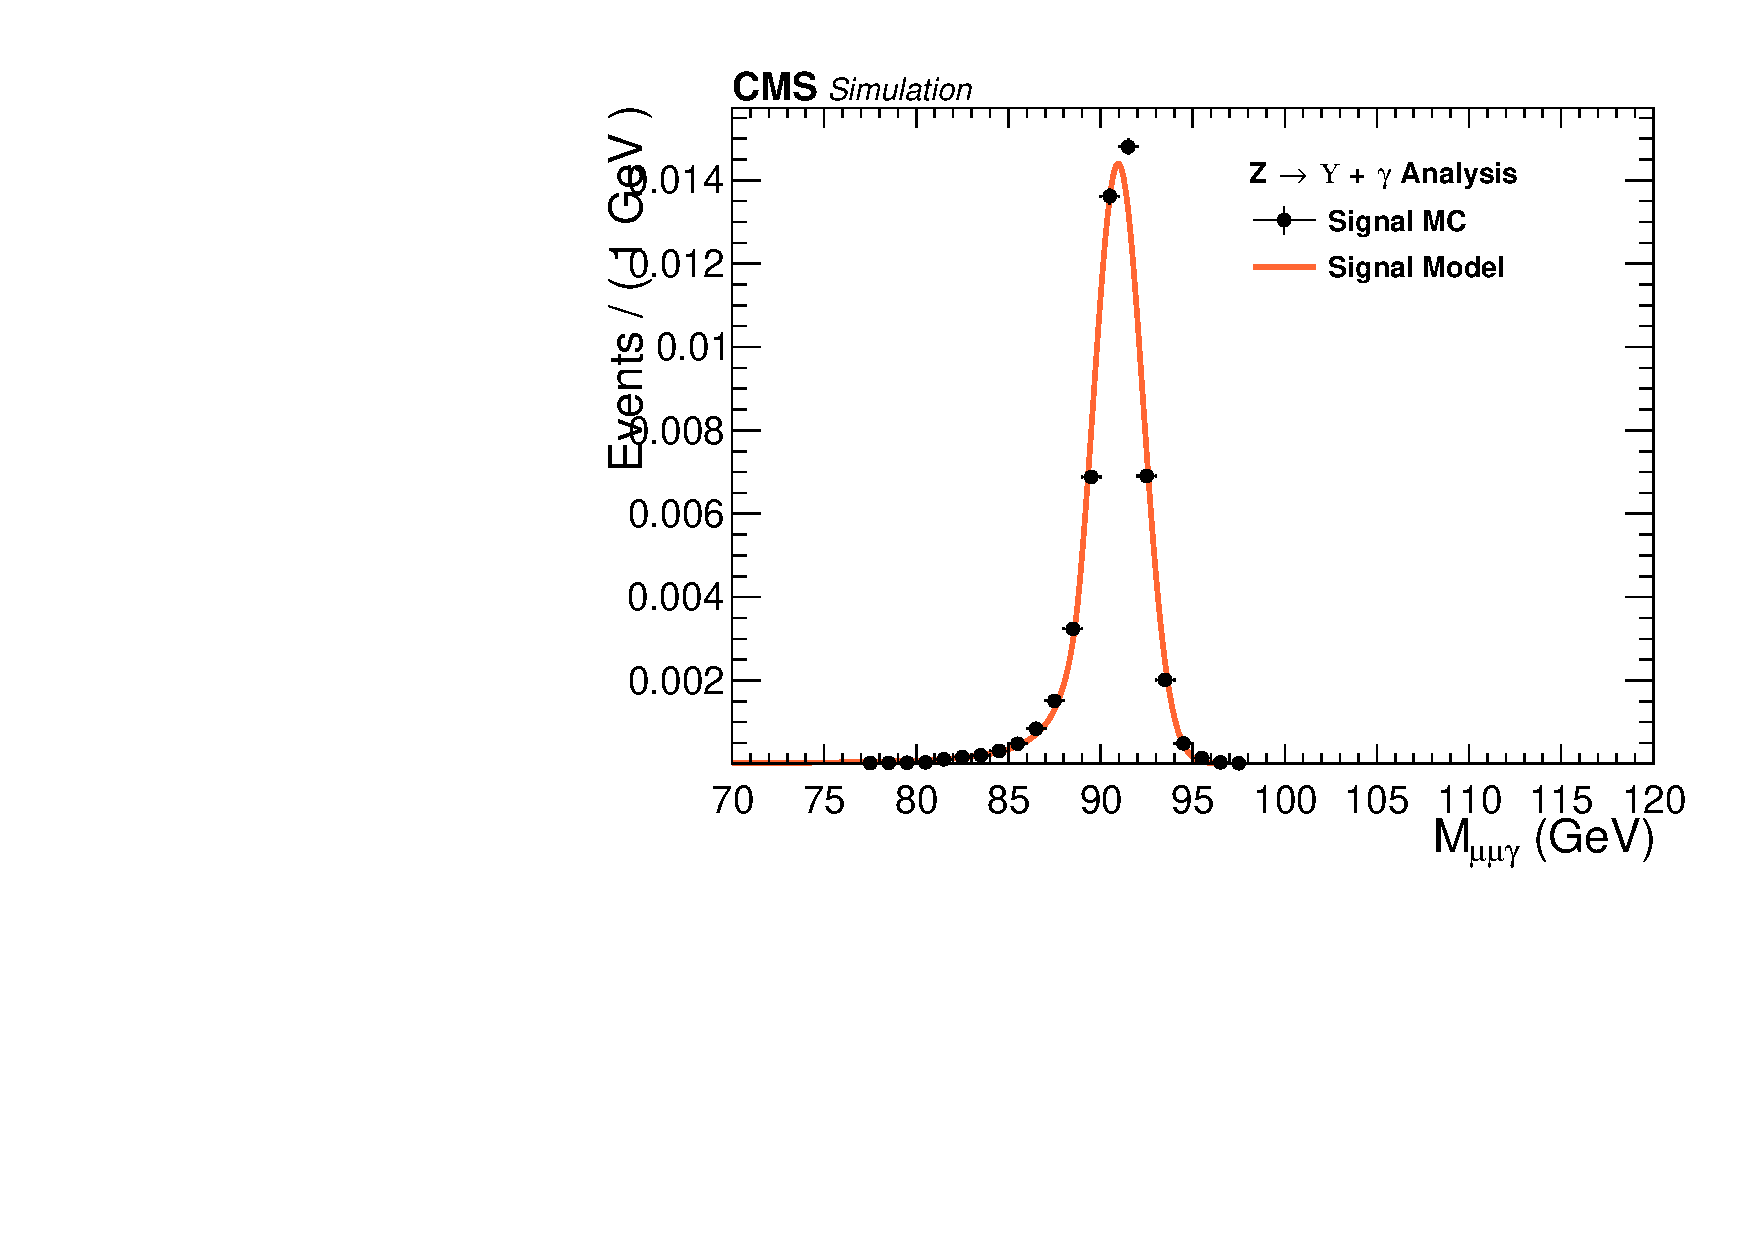
\includegraphics[width=0.45\textwidth]{figures_and_tables/fitPlotFiles2D/ZToUpsilonPhotonSignalAndBackgroundFit/mHZ_ZToUpsilon2SPhotonSignalAndBackgroundFit_Signal_Cat2_default}\hspace*{1.cm}

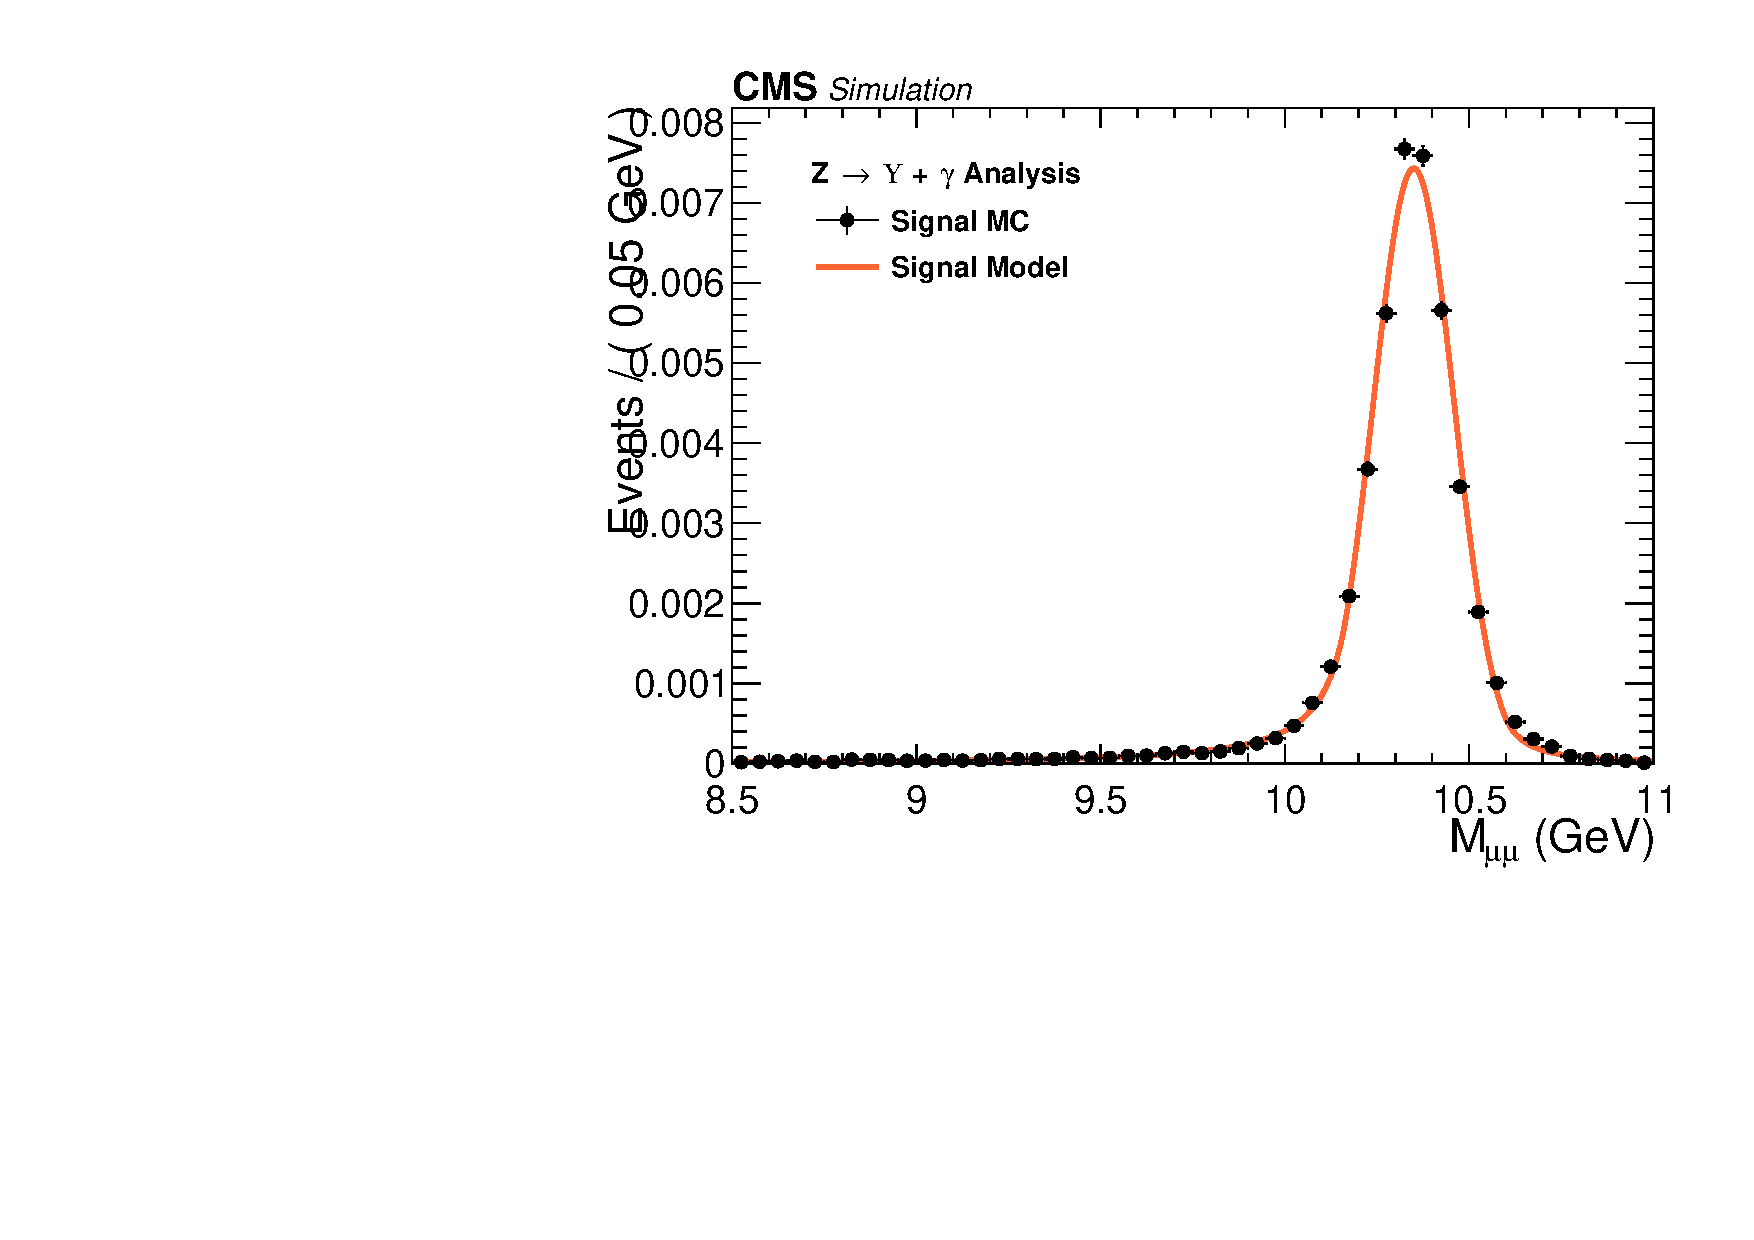
\includegraphics[width=0.45\textwidth]{figures_and_tables/fitPlotFiles2D/ZToUpsilonPhotonSignalAndBackgroundFit/mMuMNU_ZToUpsilon3SPhotonSignalAndBackgroundFit_Signal_Cat2}\hspace*{1.cm}
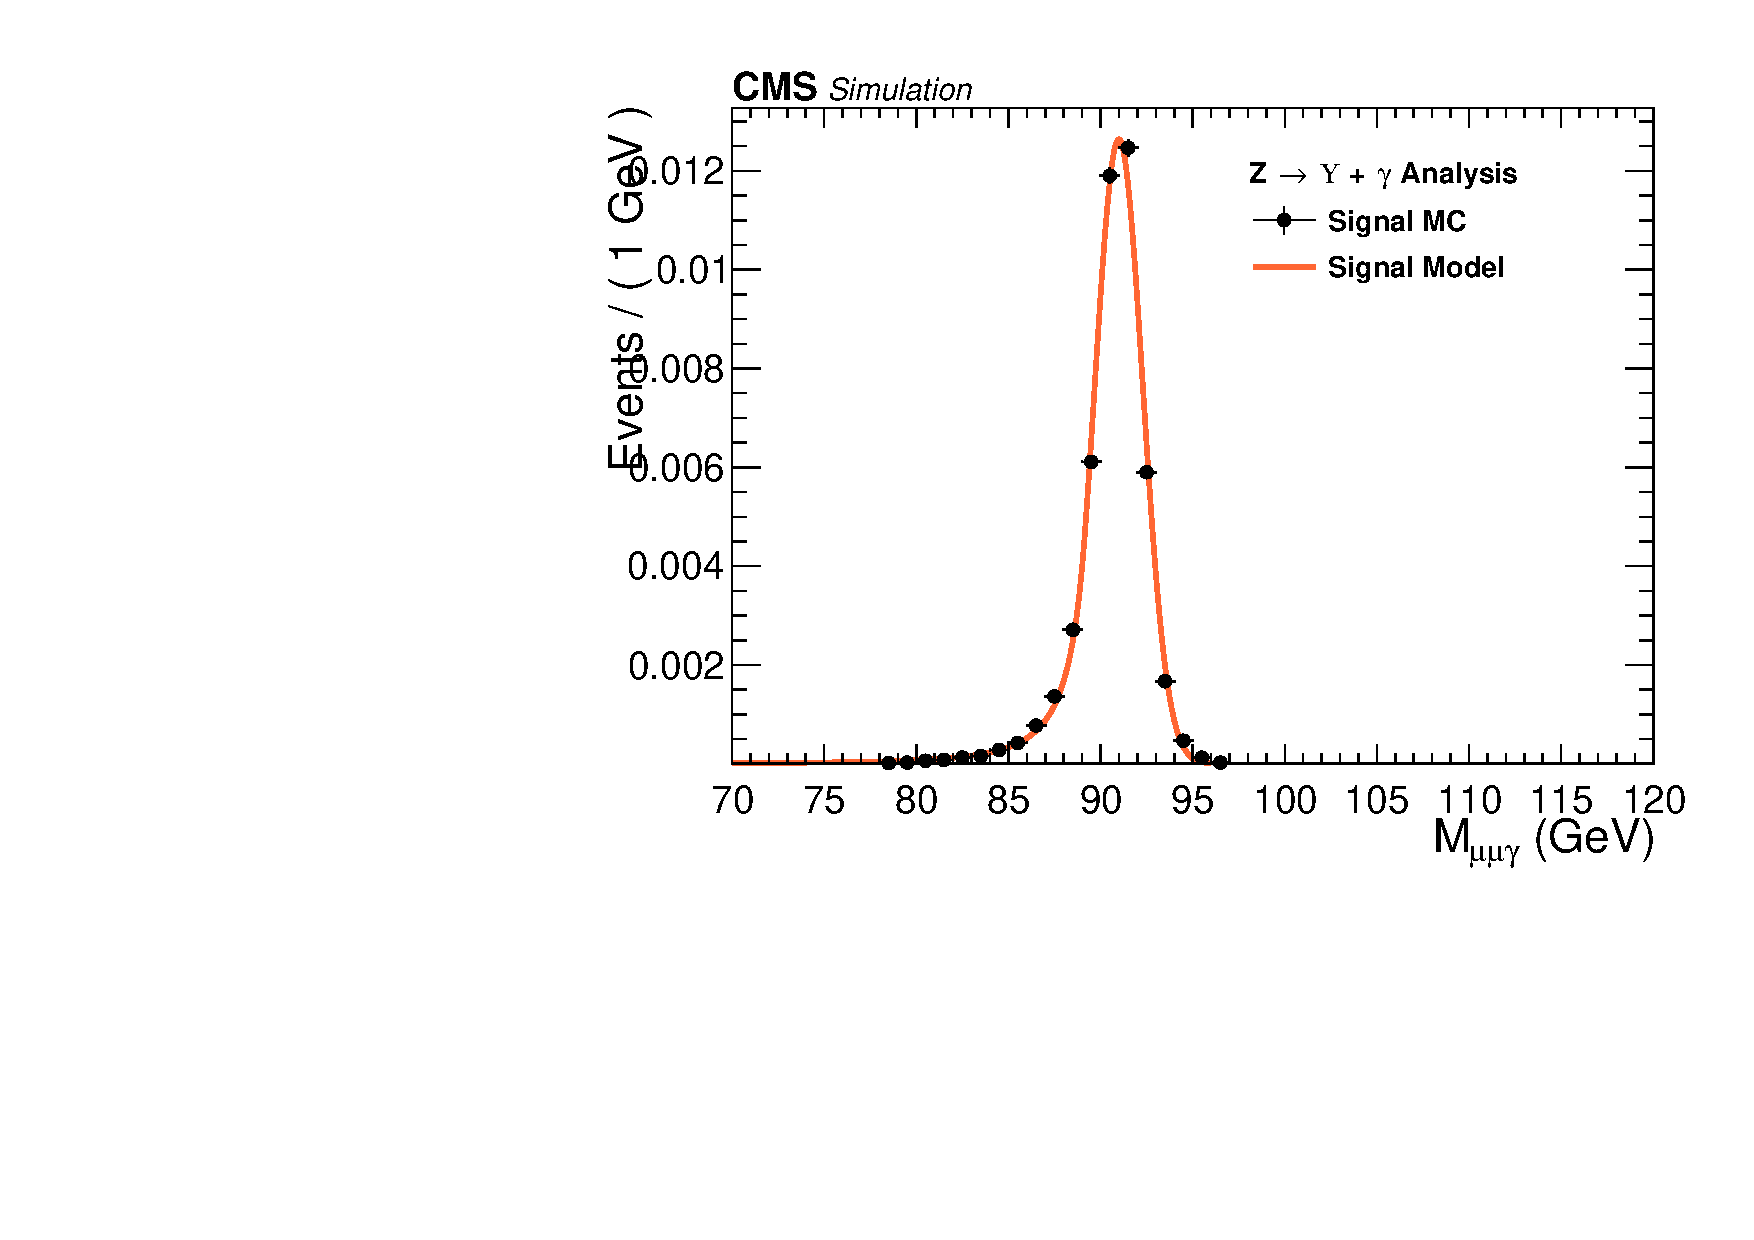
\includegraphics[width=0.45\textwidth]{figures_and_tables/fitPlotFiles2D/ZToUpsilonPhotonSignalAndBackgroundFit/mHZ_ZToUpsilon3SPhotonSignalAndBackgroundFit_Signal_Cat2_default}\hspace*{1.cm}


\end{center}\vspace*{-.5cm}
\caption{Signal Modeling for the $Z \rightarrow \Upsilon(1S,2S,3S) +\gamma$ analysis for EB Low R9 category. $m_{\mu\mu}$ mass distribution (left) and $m_{\mu\mu\gamma}$ mass distribution (right). From top to bottom: $\Upsilon(1S)$, $\Upsilon(2S)$, $\Upsilon(3S)$.}
\label{fig:ZToUpsilon_Signal_Cat2}
\end{figure}

% Cat3
\begin{figure}[!htbp]
\begin{center}


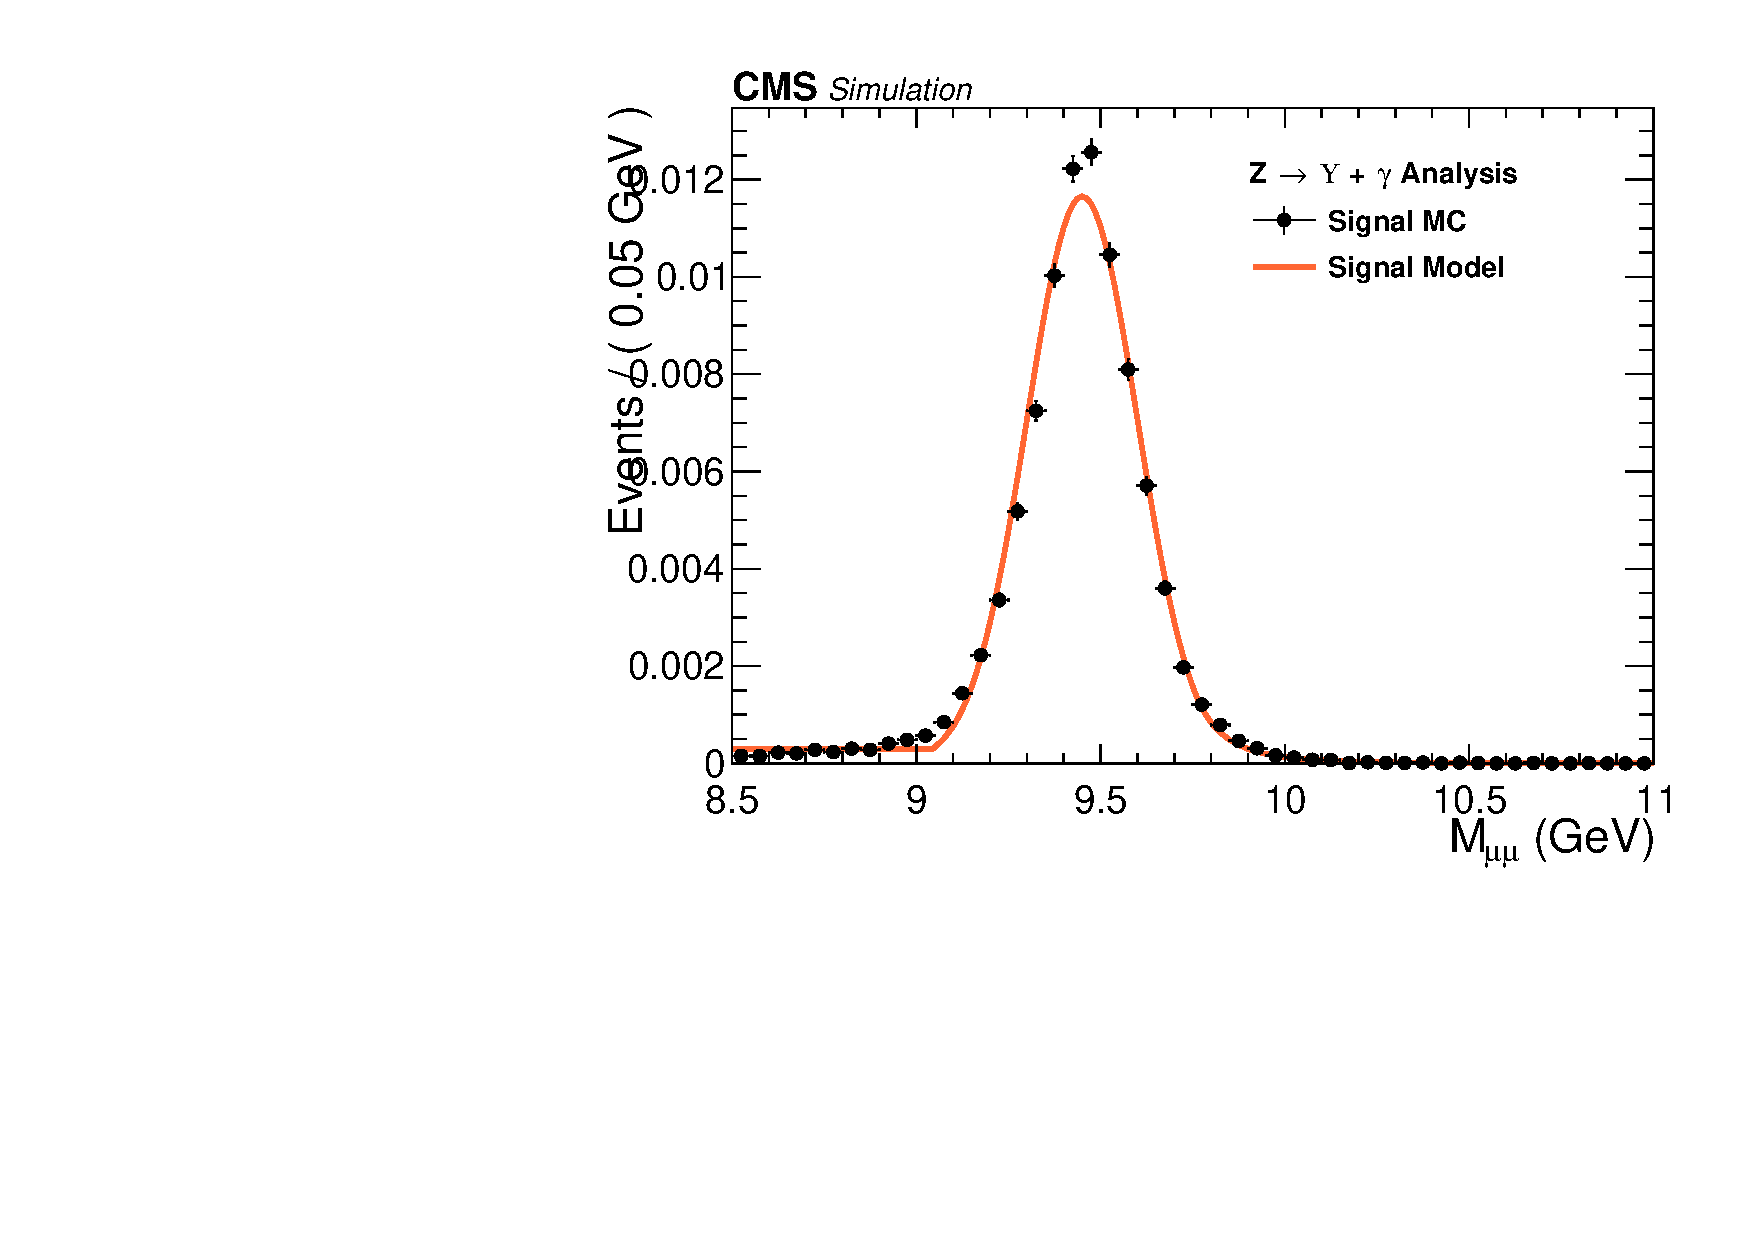
\includegraphics[width=0.45\textwidth]{figures_and_tables/fitPlotFiles2D/ZToUpsilonPhotonSignalAndBackgroundFit/mMuMNU_ZToUpsilon1SPhotonSignalAndBackgroundFit_Signal_Cat3}\hspace*{1.cm}
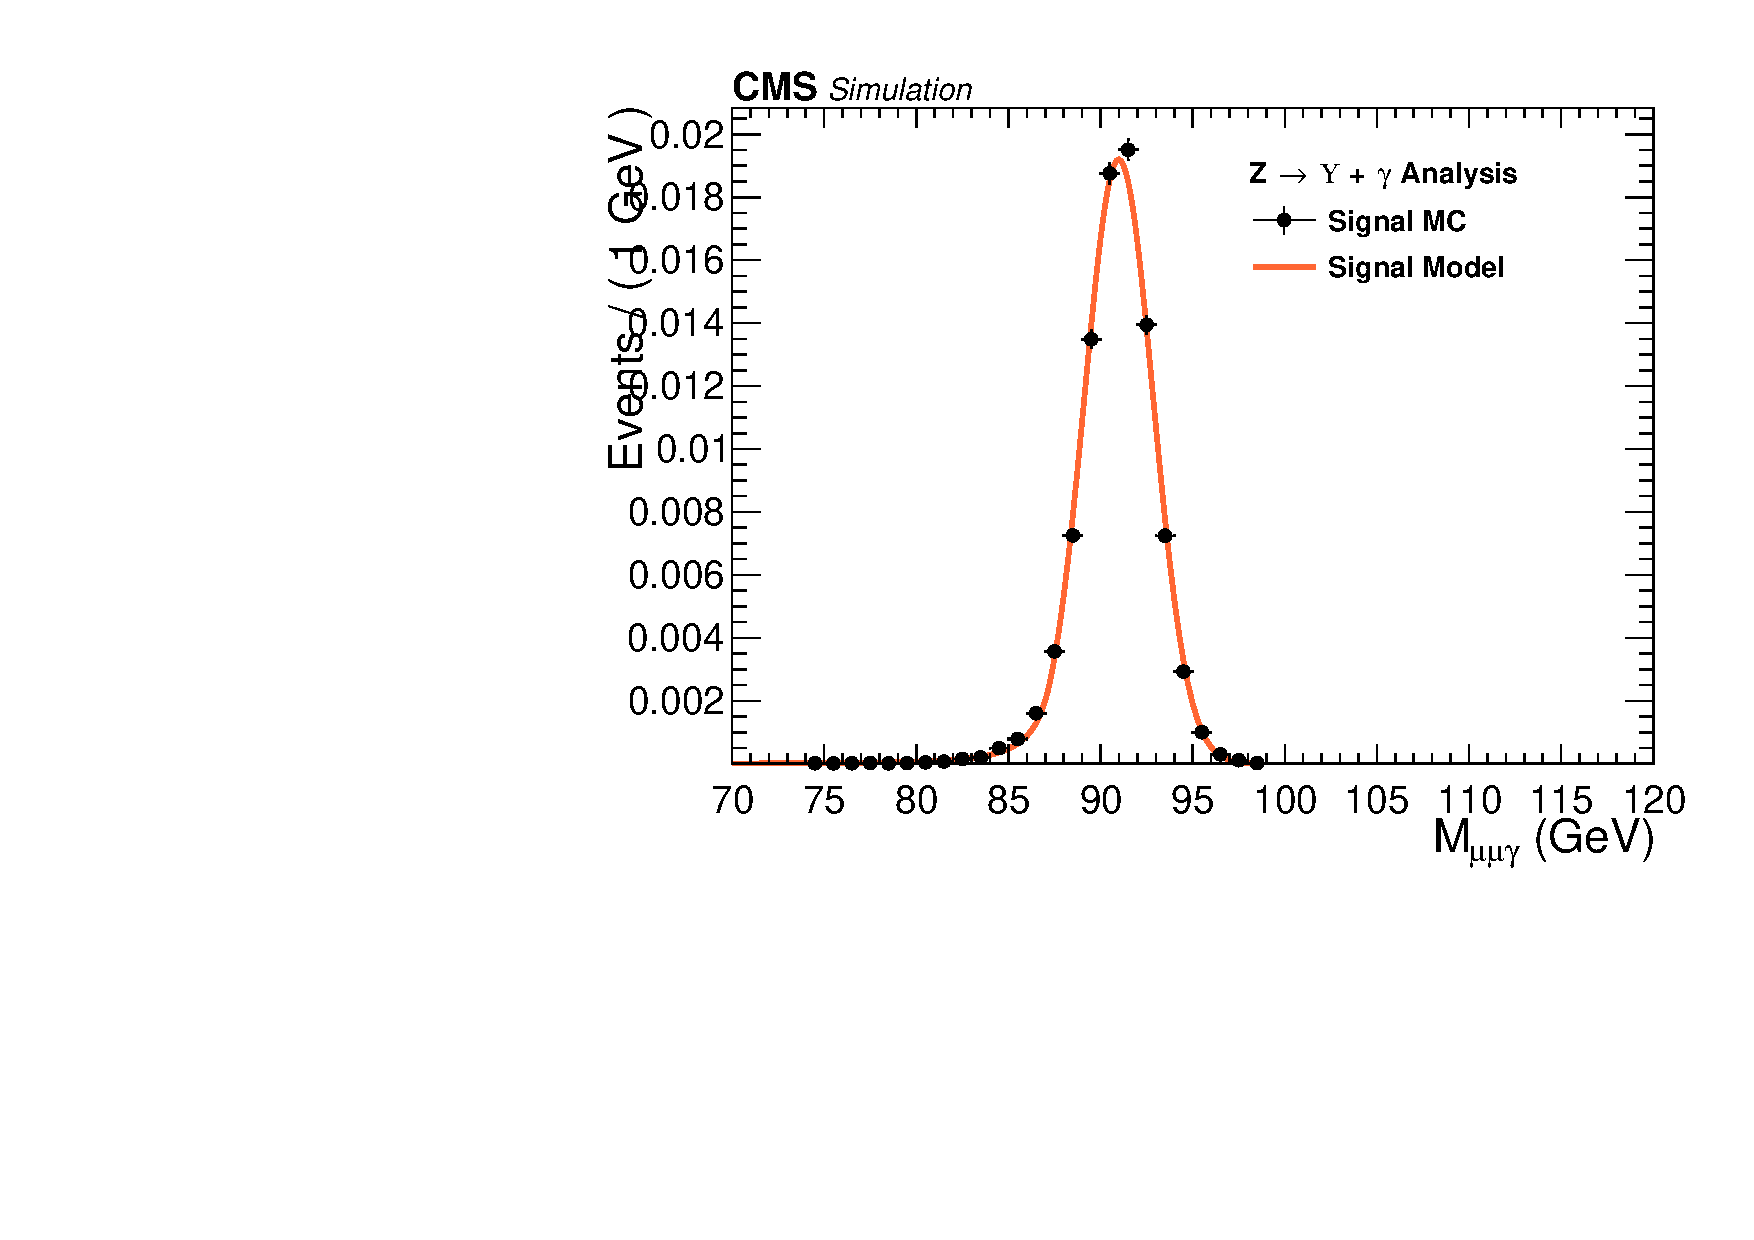
\includegraphics[width=0.45\textwidth]{figures_and_tables/fitPlotFiles2D/ZToUpsilonPhotonSignalAndBackgroundFit/mHZ_ZToUpsilon1SPhotonSignalAndBackgroundFit_Signal_Cat3_default}\hspace*{1.cm}

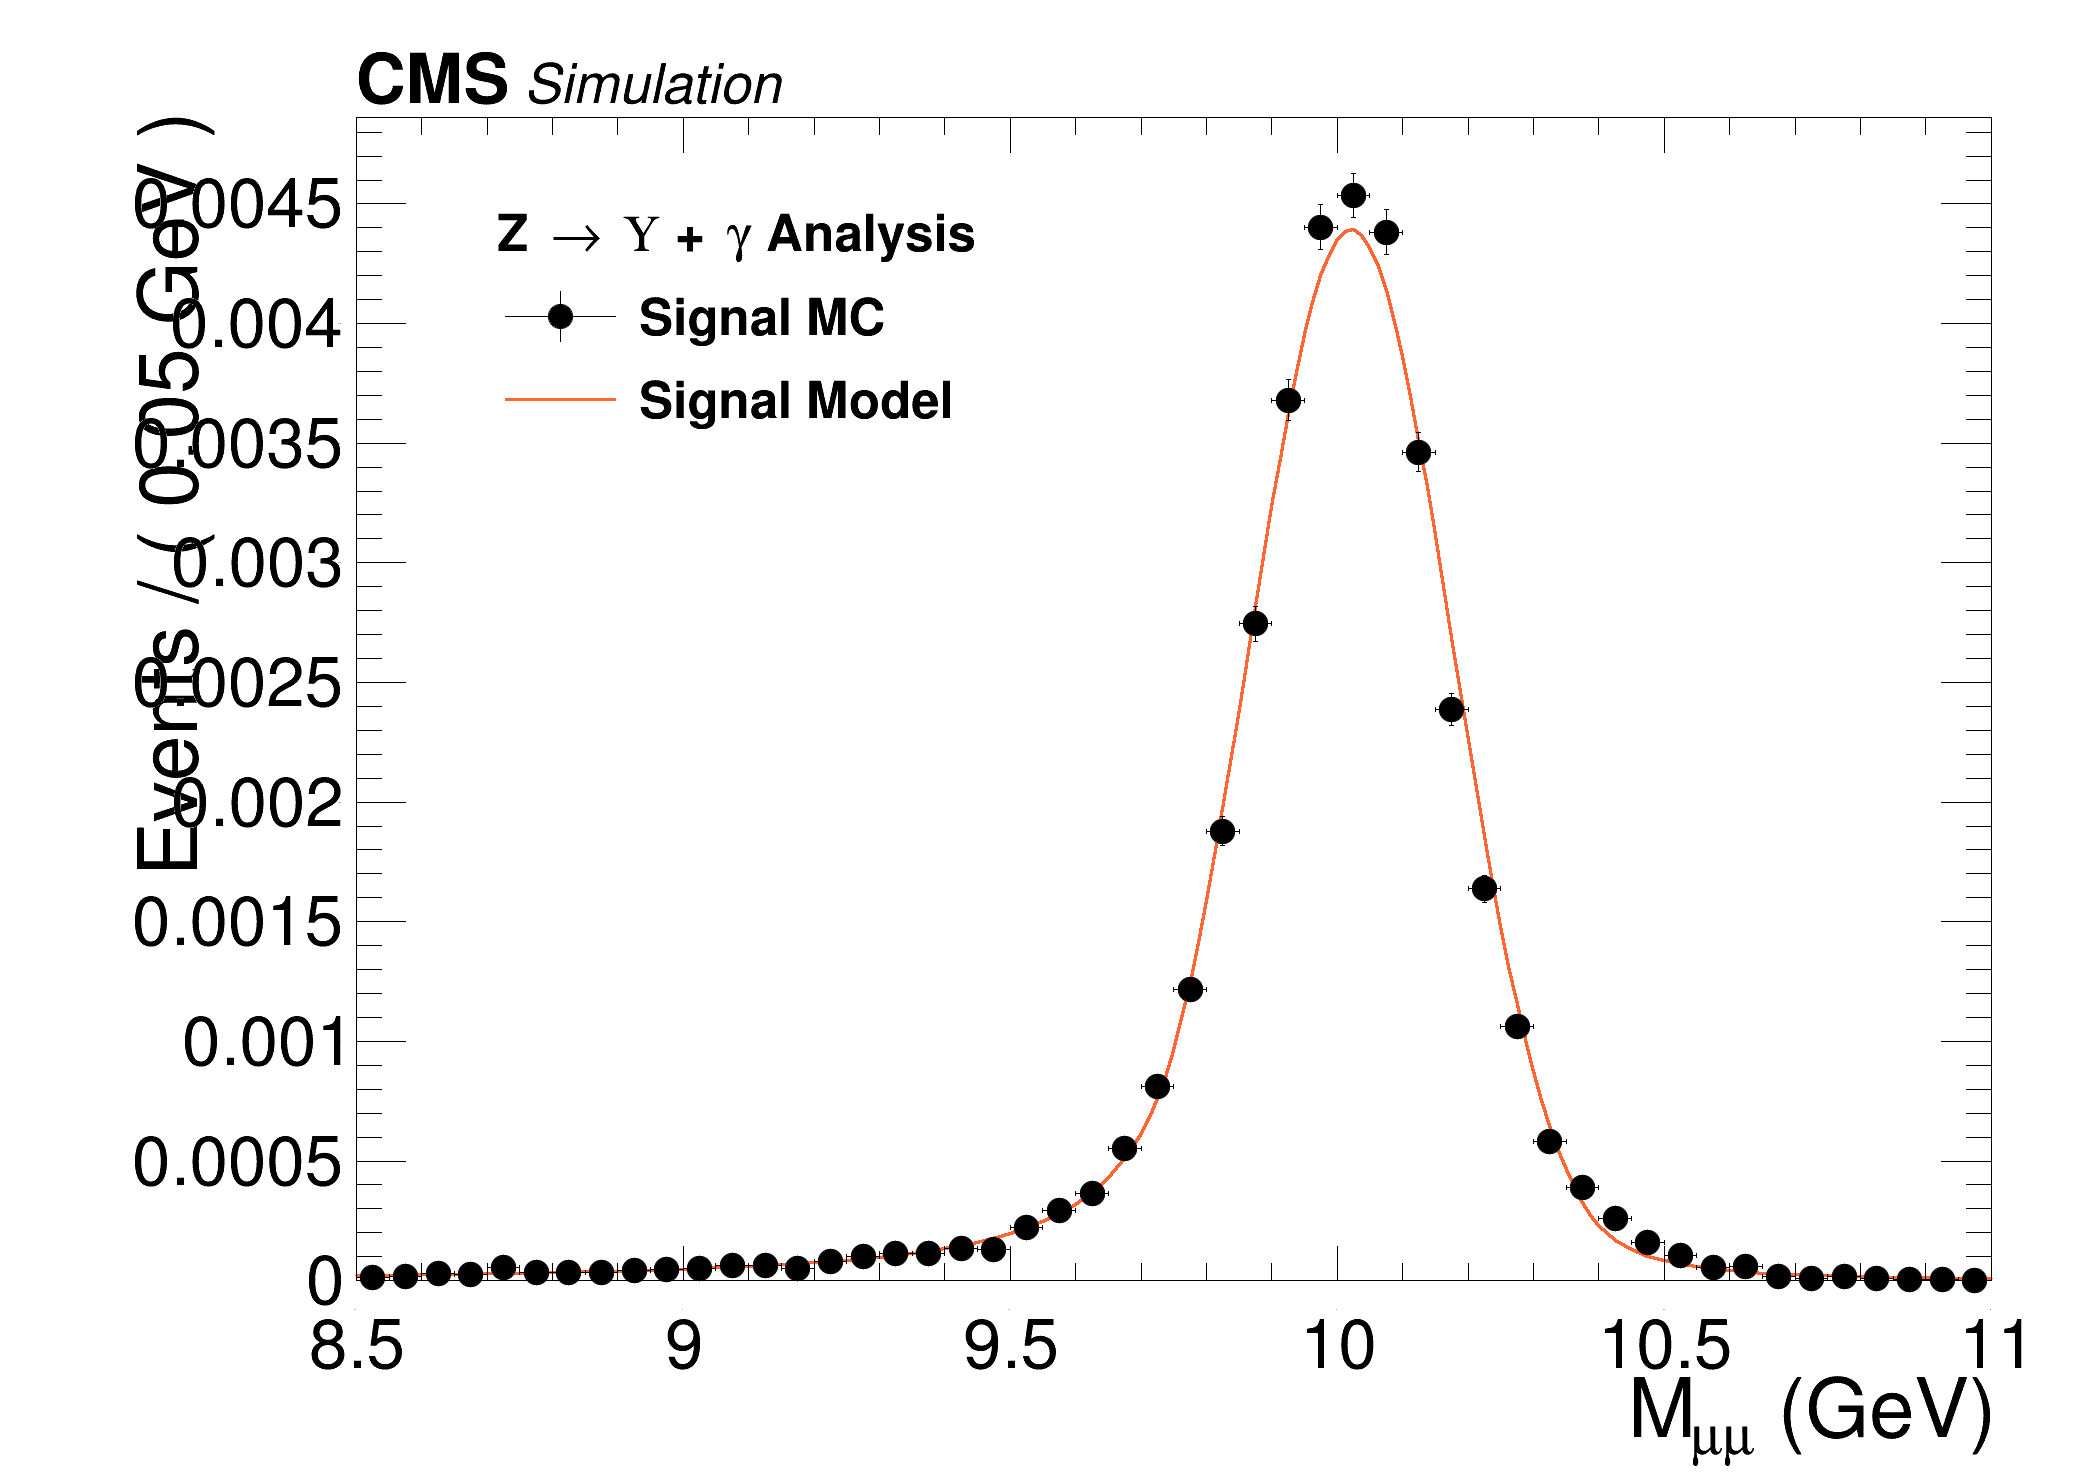
\includegraphics[width=0.45\textwidth]{figures_and_tables/fitPlotFiles2D/ZToUpsilonPhotonSignalAndBackgroundFit/mMuMNU_ZToUpsilon2SPhotonSignalAndBackgroundFit_Signal_Cat3}\hspace*{1.cm}
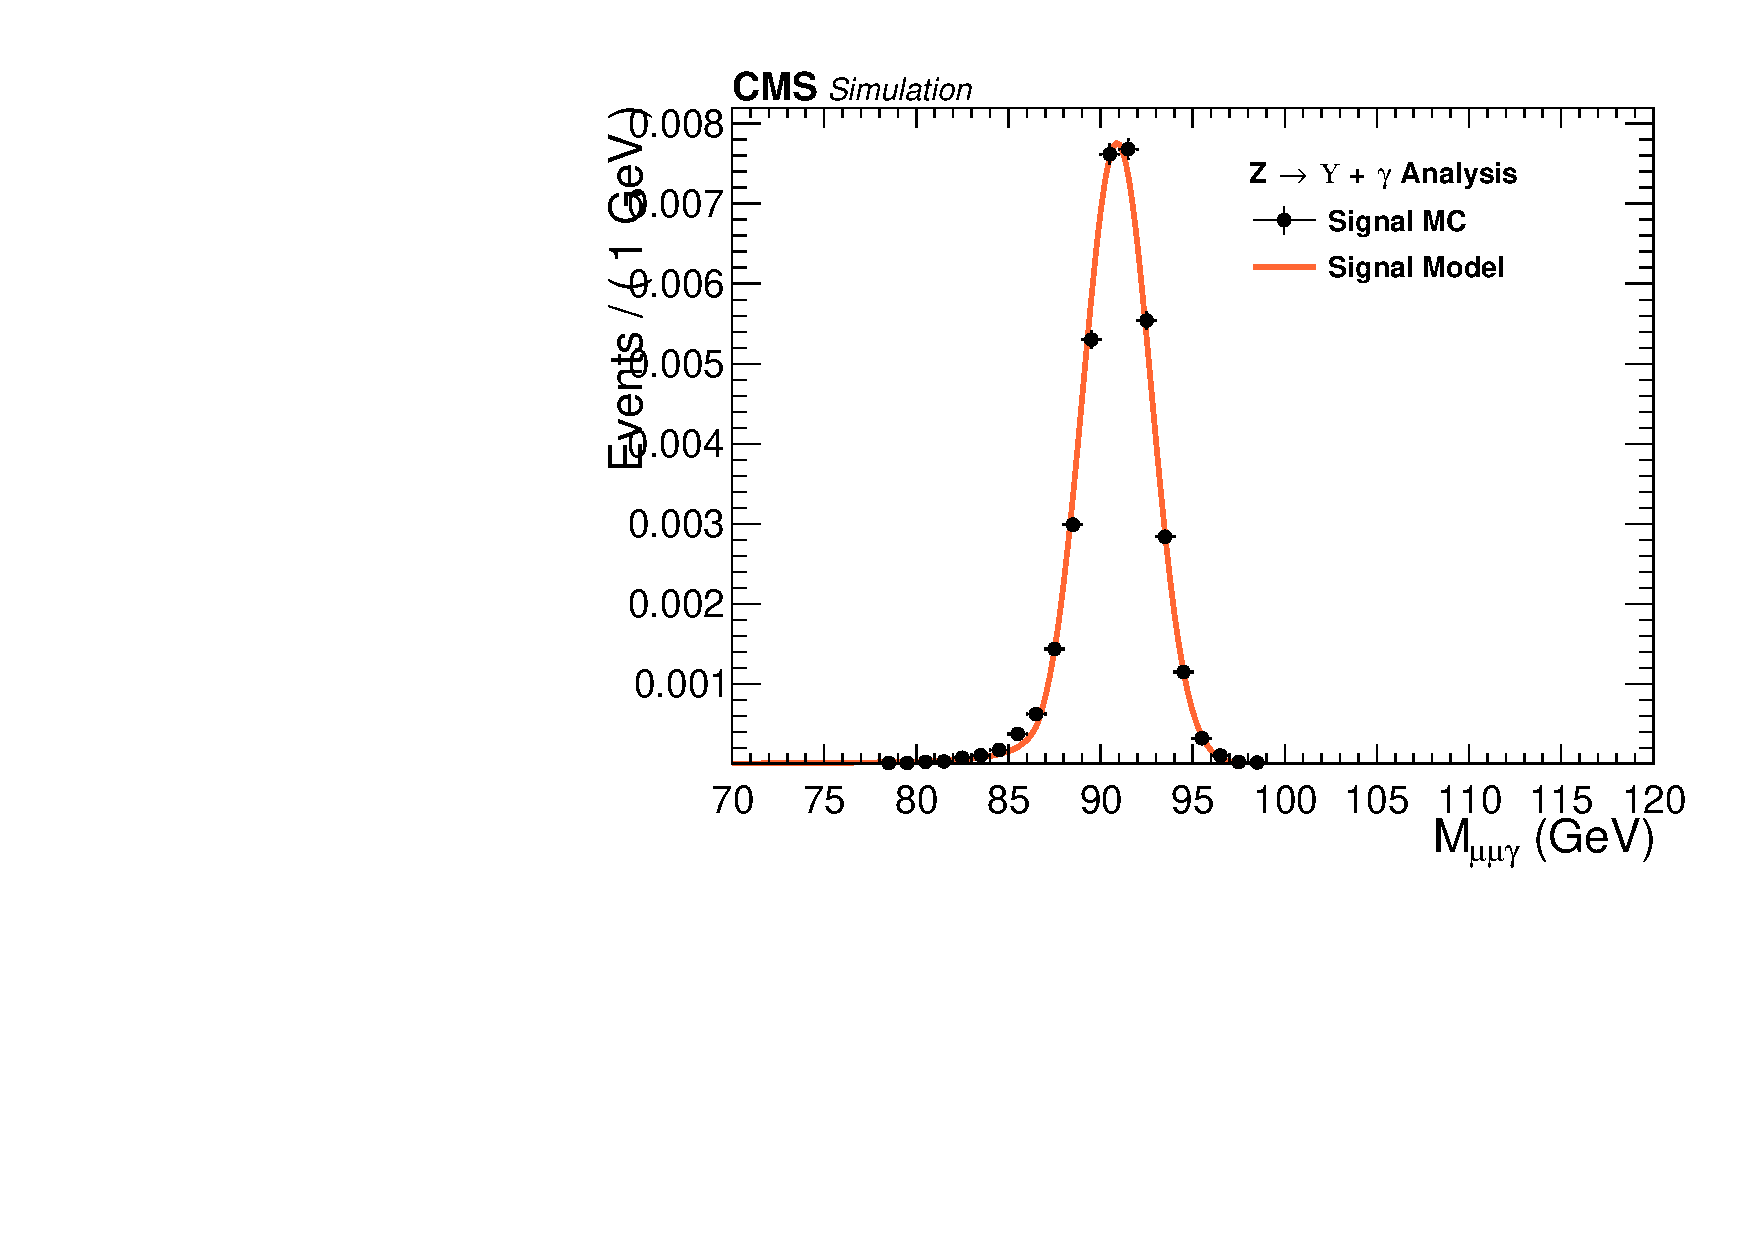
\includegraphics[width=0.45\textwidth]{figures_and_tables/fitPlotFiles2D/ZToUpsilonPhotonSignalAndBackgroundFit/mHZ_ZToUpsilon2SPhotonSignalAndBackgroundFit_Signal_Cat3_default}\hspace*{1.cm}

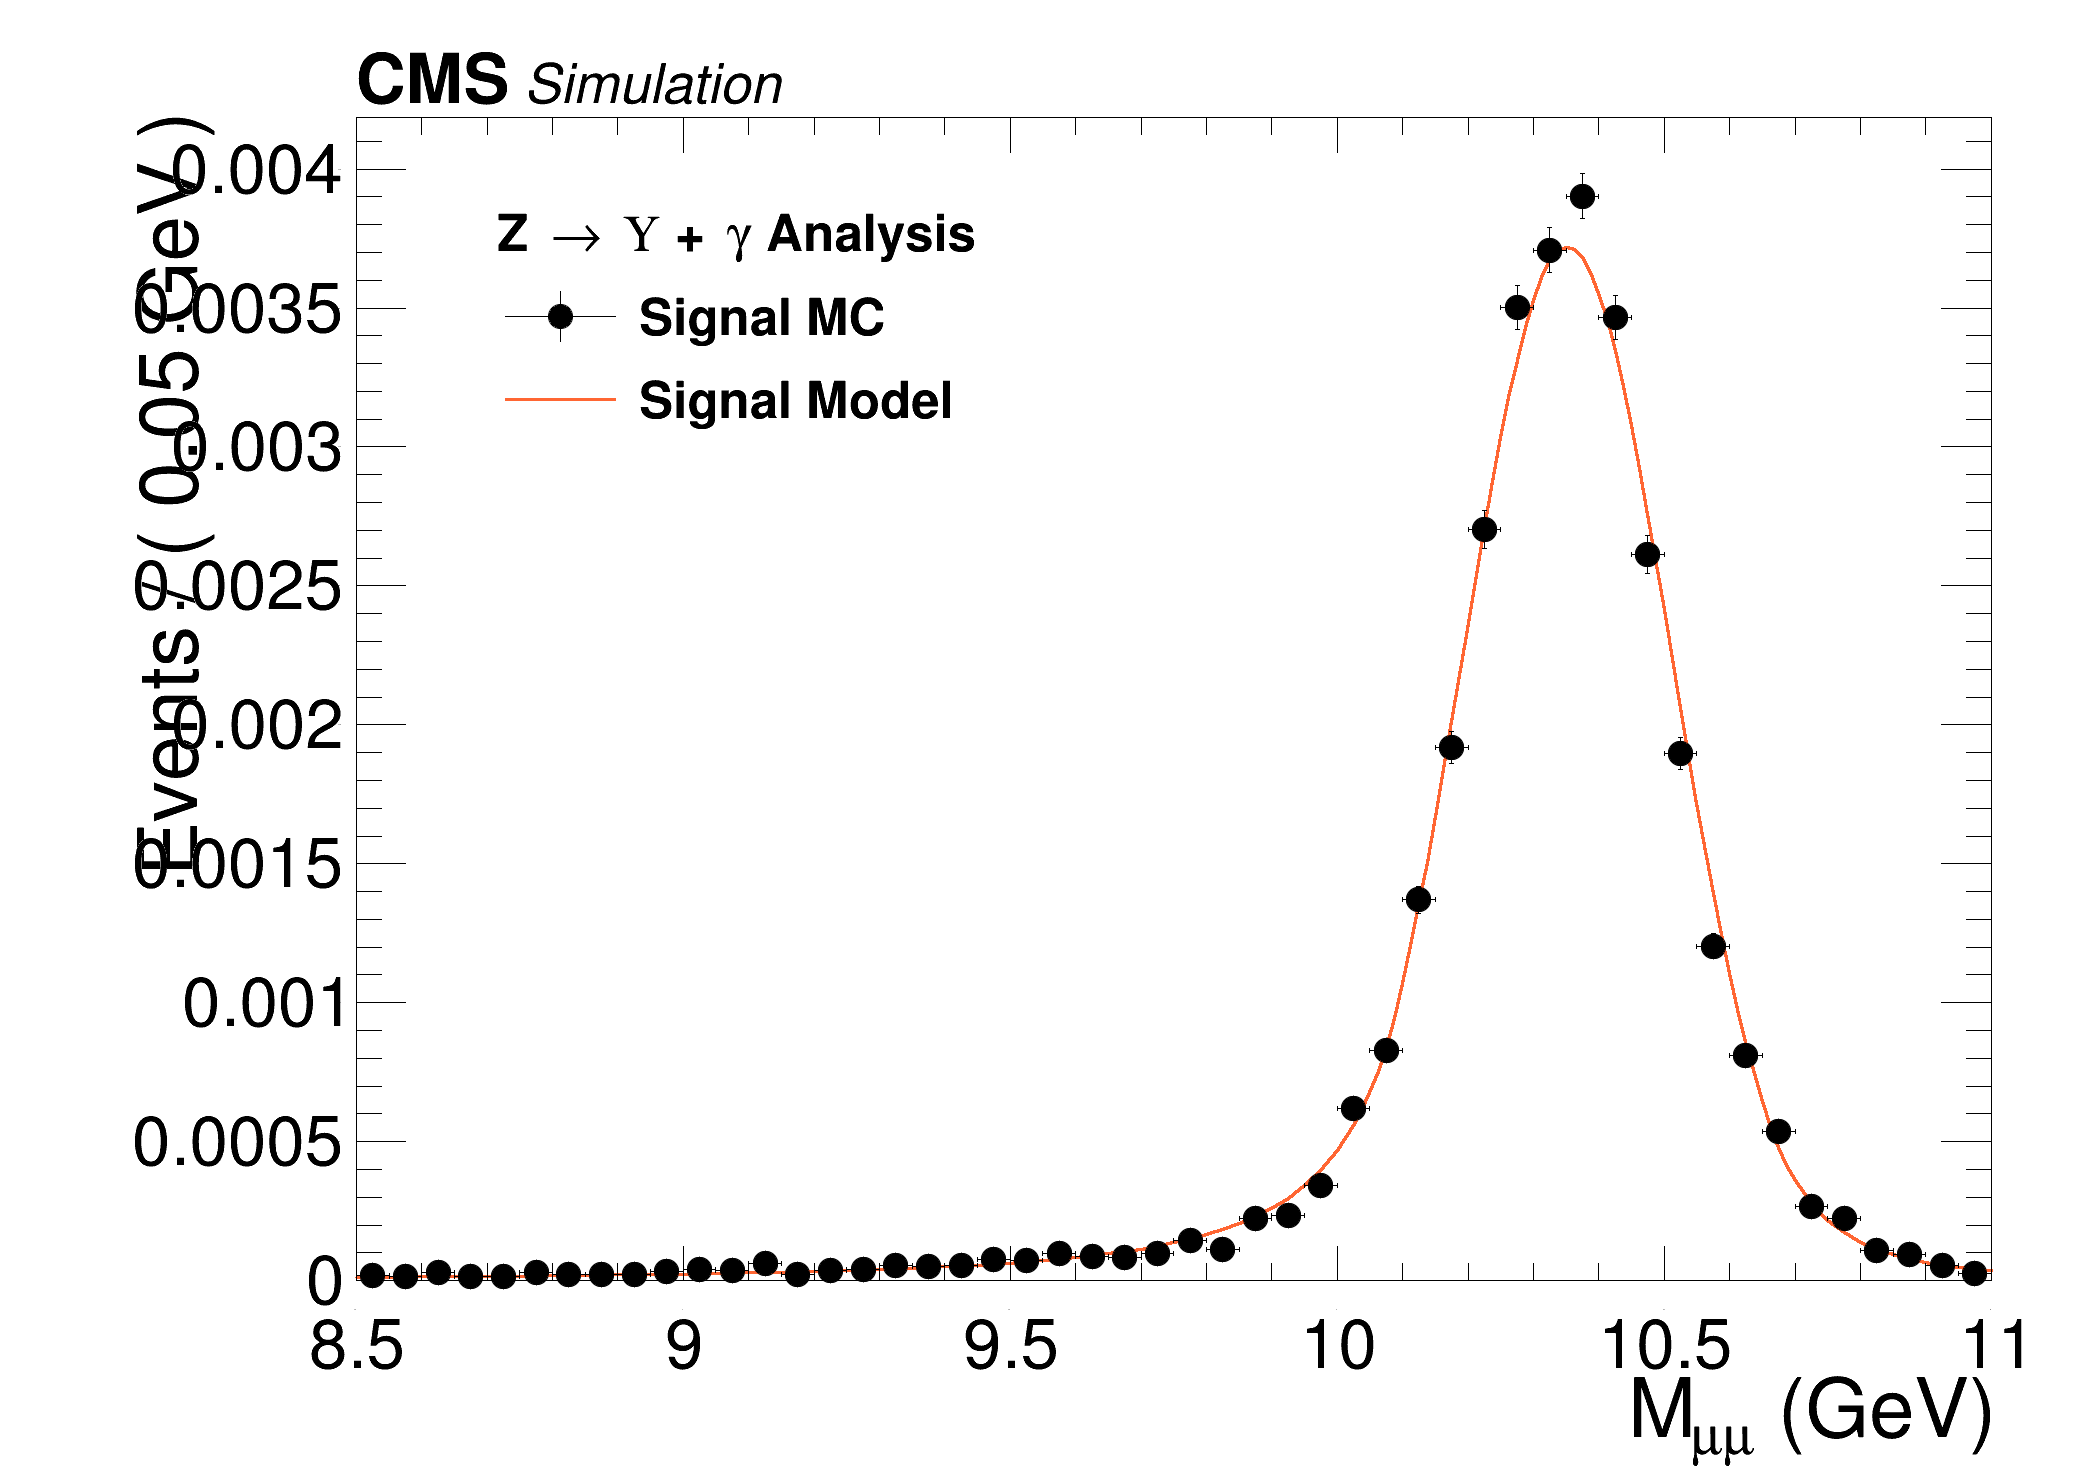
\includegraphics[width=0.45\textwidth]{figures_and_tables/fitPlotFiles2D/ZToUpsilonPhotonSignalAndBackgroundFit/mMuMNU_ZToUpsilon3SPhotonSignalAndBackgroundFit_Signal_Cat3}\hspace*{1.cm}
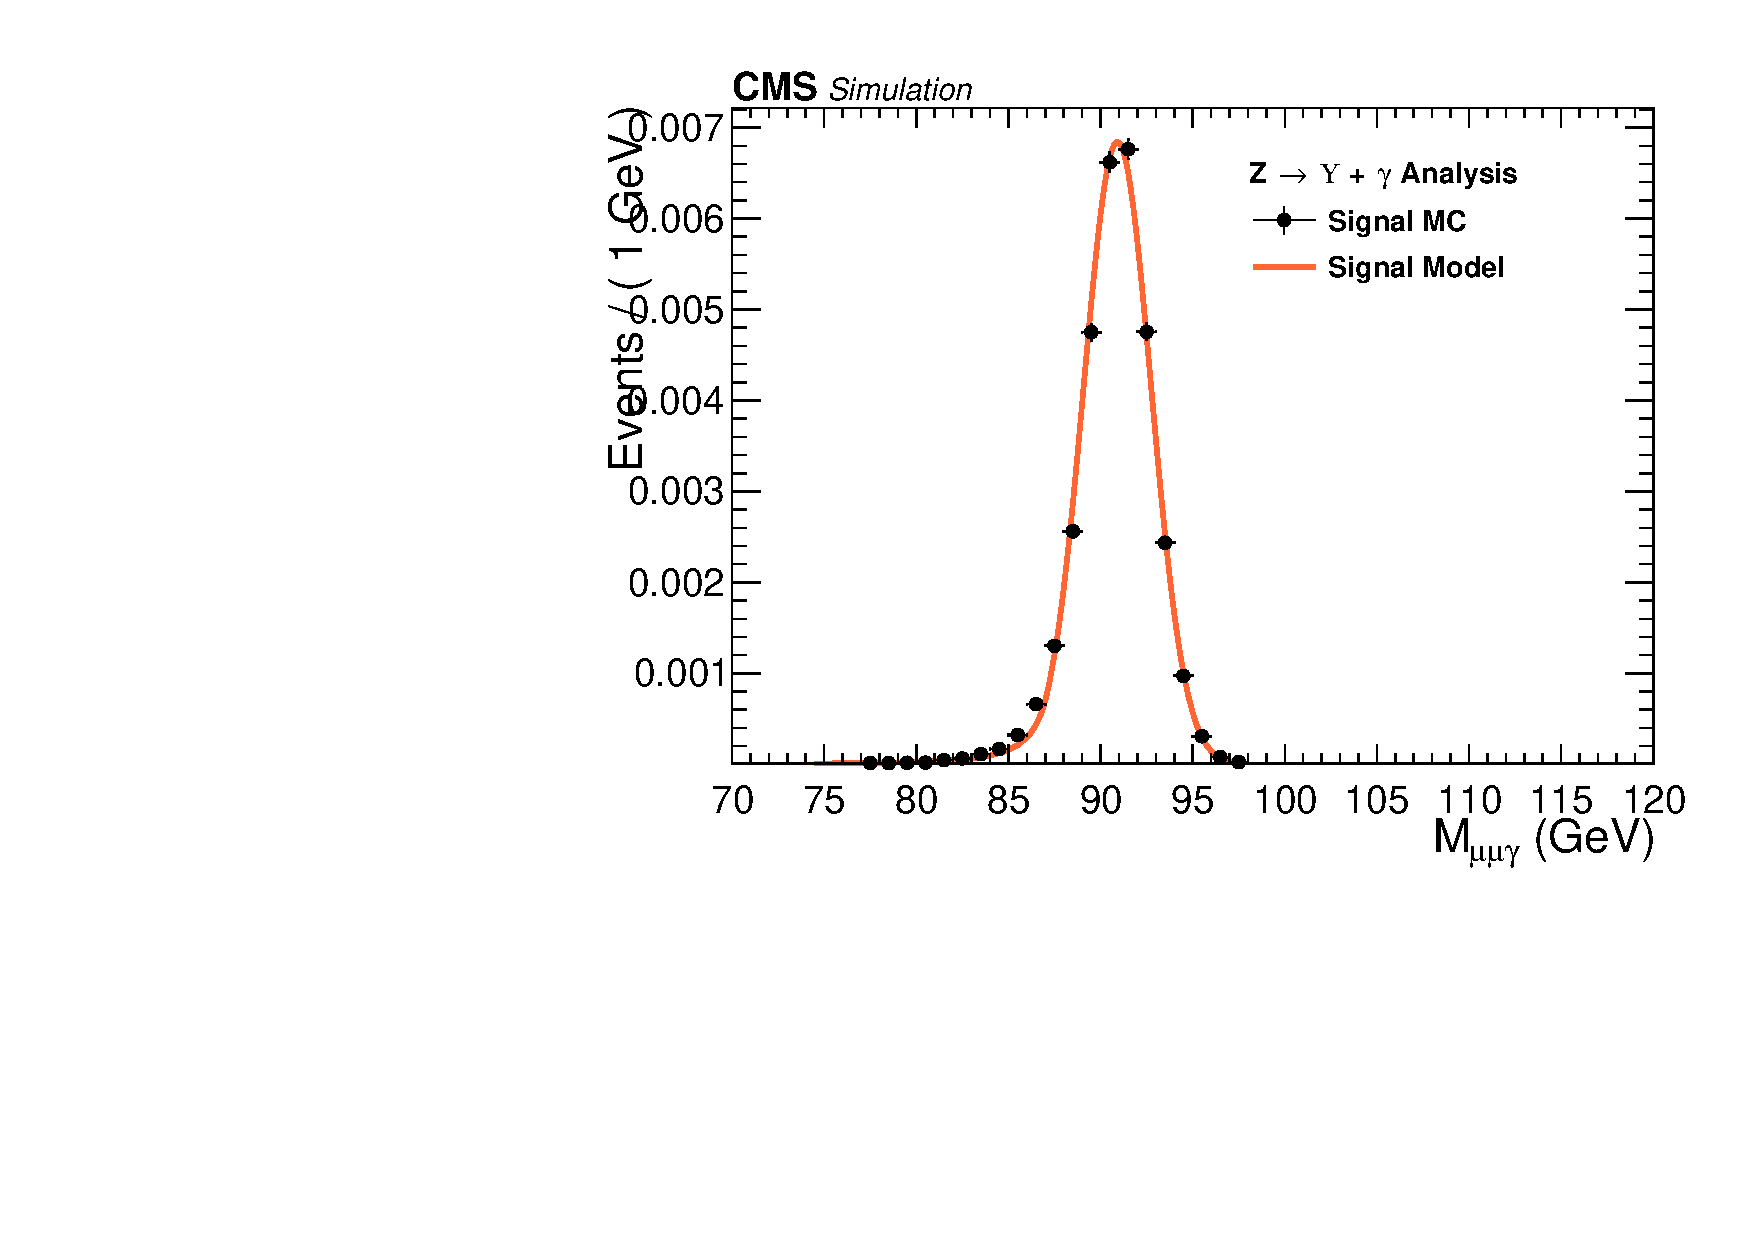
\includegraphics[width=0.45\textwidth]{figures_and_tables/fitPlotFiles2D/ZToUpsilonPhotonSignalAndBackgroundFit/mHZ_ZToUpsilon3SPhotonSignalAndBackgroundFit_Signal_Cat3_default}\hspace*{1.cm}


\end{center}\vspace*{-.5cm}
\caption{Signal Modeling for the $Z \rightarrow \Upsilon(1S,2S,3S) +\gamma$ analysis for EE category. $m_{\mu\mu}$ mass distribution (left) and $m_{\mu\mu\gamma}$ mass distribution (right). From top to bottom: $\Upsilon(1S)$, $\Upsilon(2S)$, $\Upsilon(3S)$.}
\label{fig:ZToUpsilon_Signal_Cat3}
\end{figure}

% H To Upsilon - Signal Modeling
% Cat0
\begin{figure}[!htbp]
\begin{center}


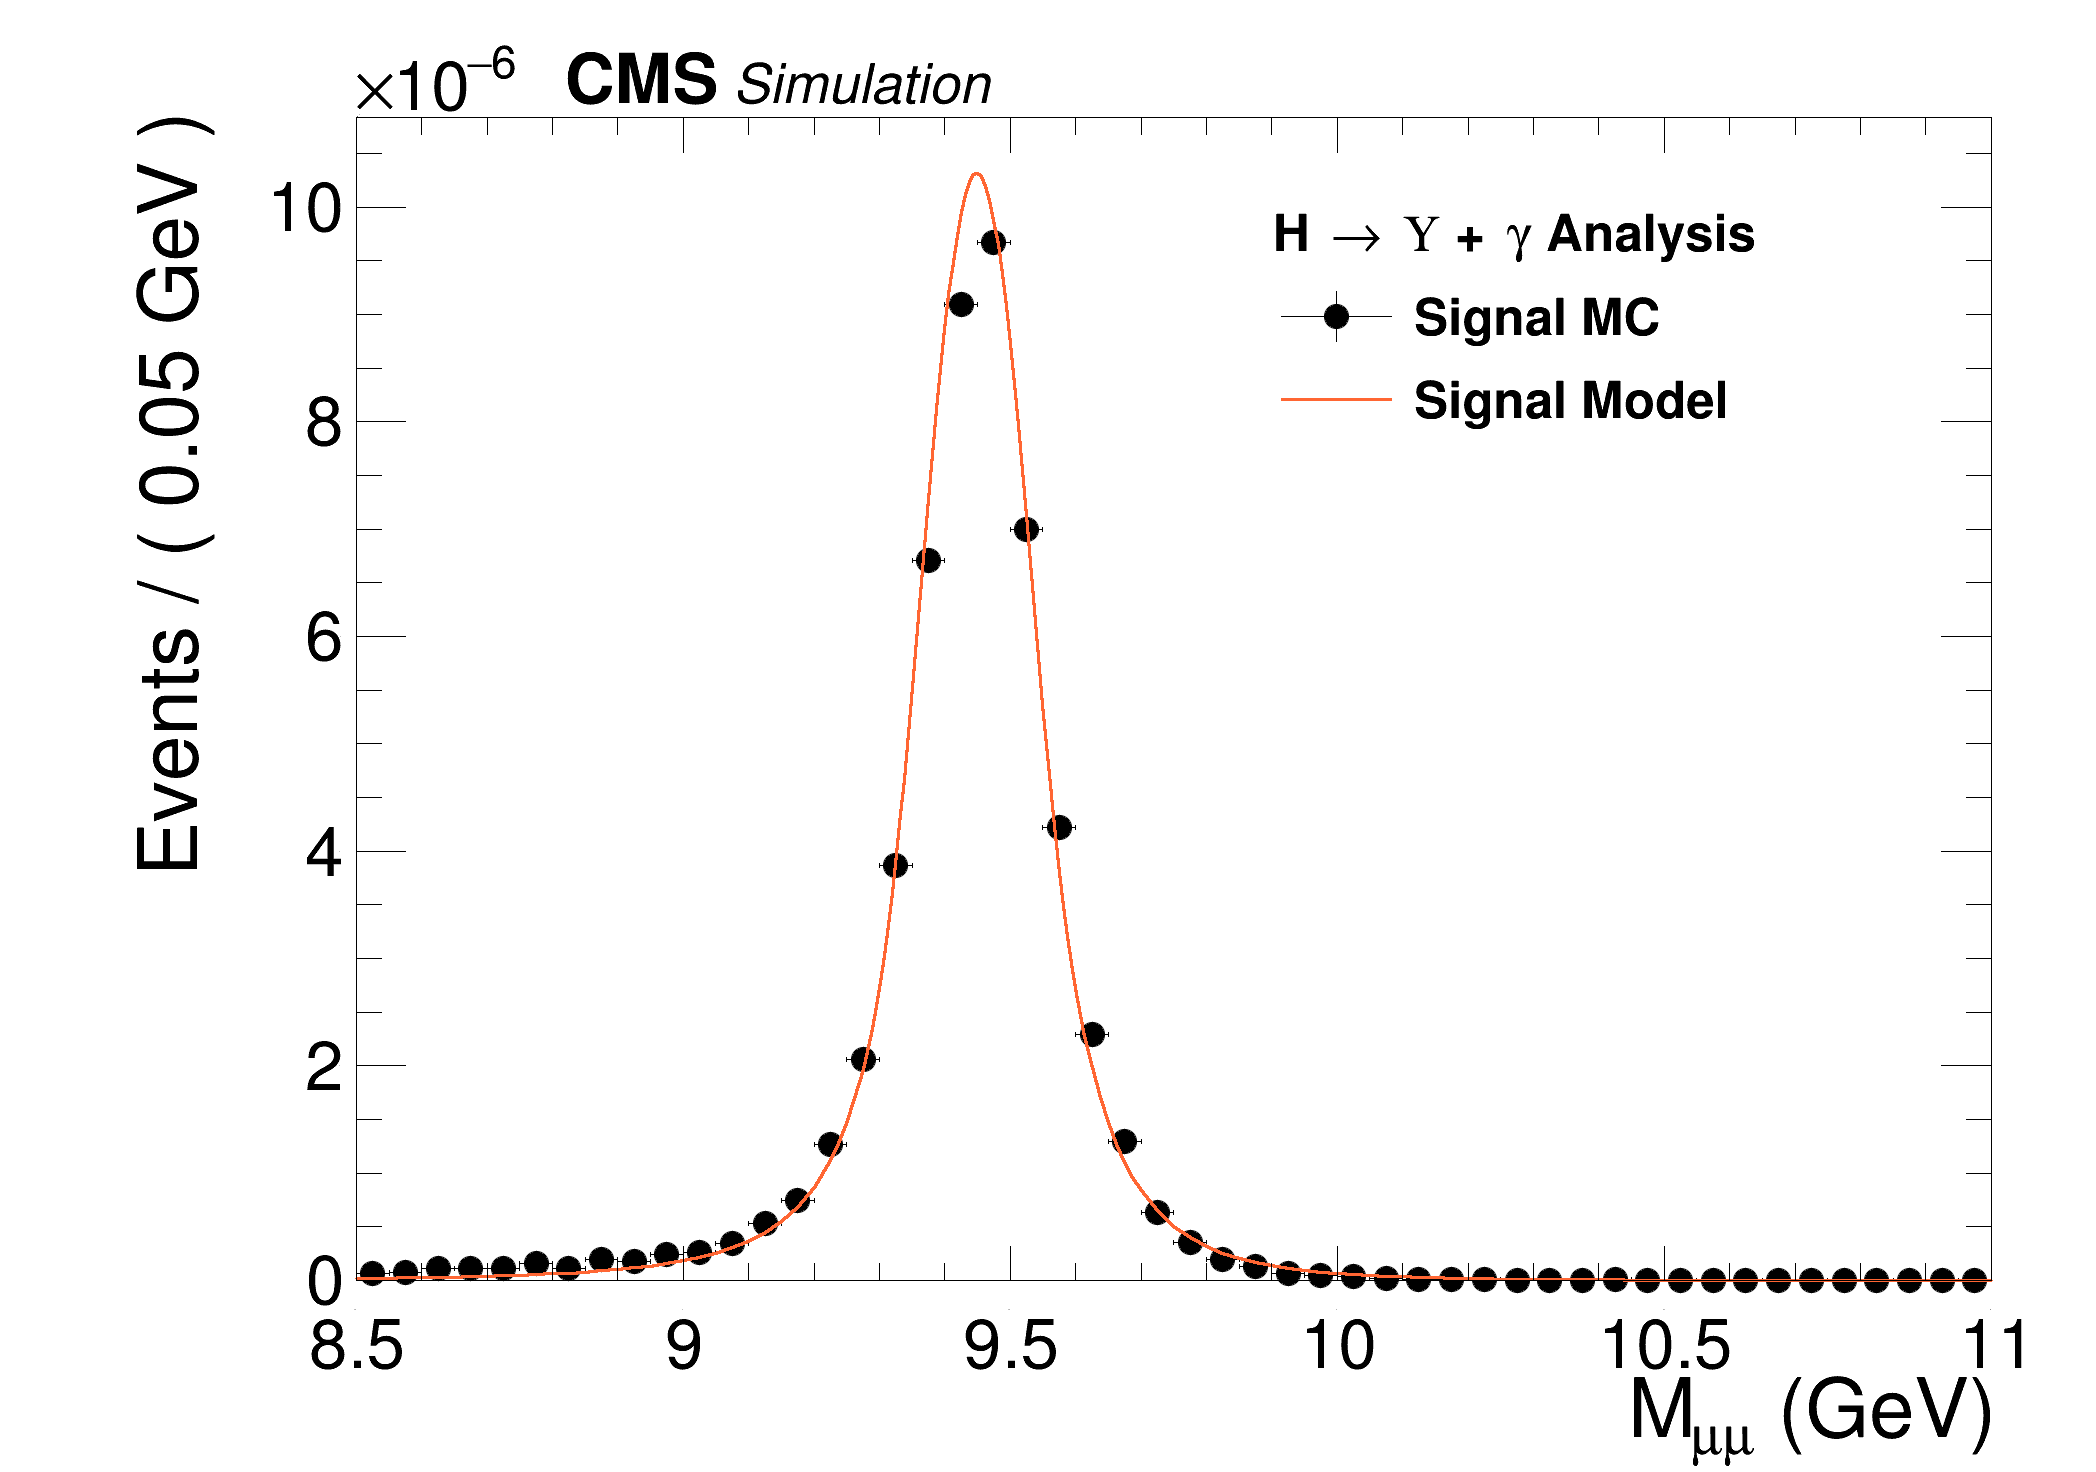
\includegraphics[width=0.45\textwidth]{figures_and_tables/fitPlotFiles2D/HToUpsilonPhotonSignalAndBackgroundFit/mMuMNU_HToUpsilon1SPhotonSignalAndBackgroundFit_Signal_Cat0}\hspace*{1.cm}
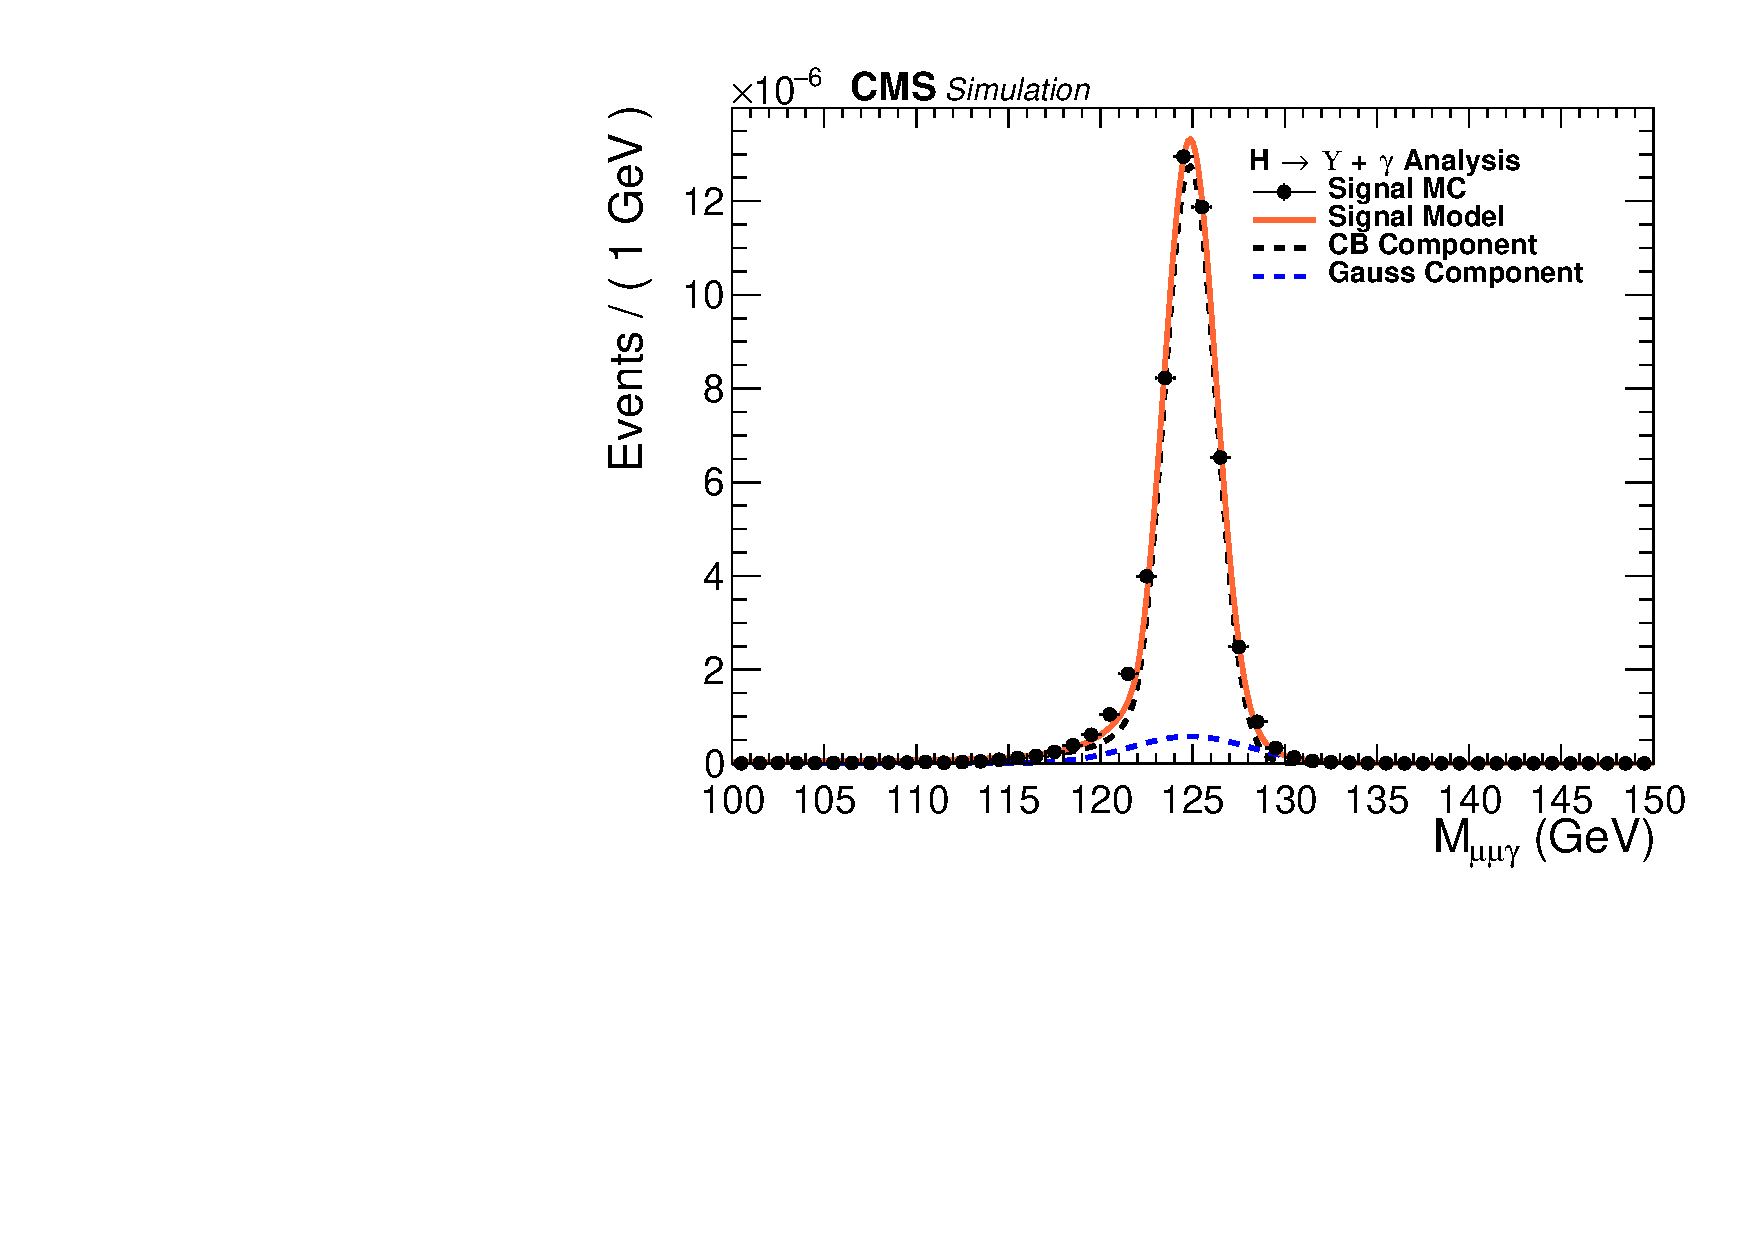
\includegraphics[width=0.45\textwidth]{figures_and_tables/fitPlotFiles2D/HToUpsilonPhotonSignalAndBackgroundFit/mHZ_HToUpsilon1SPhotonSignalAndBackgroundFit_Signal_Cat0_default}\hspace*{1.cm}

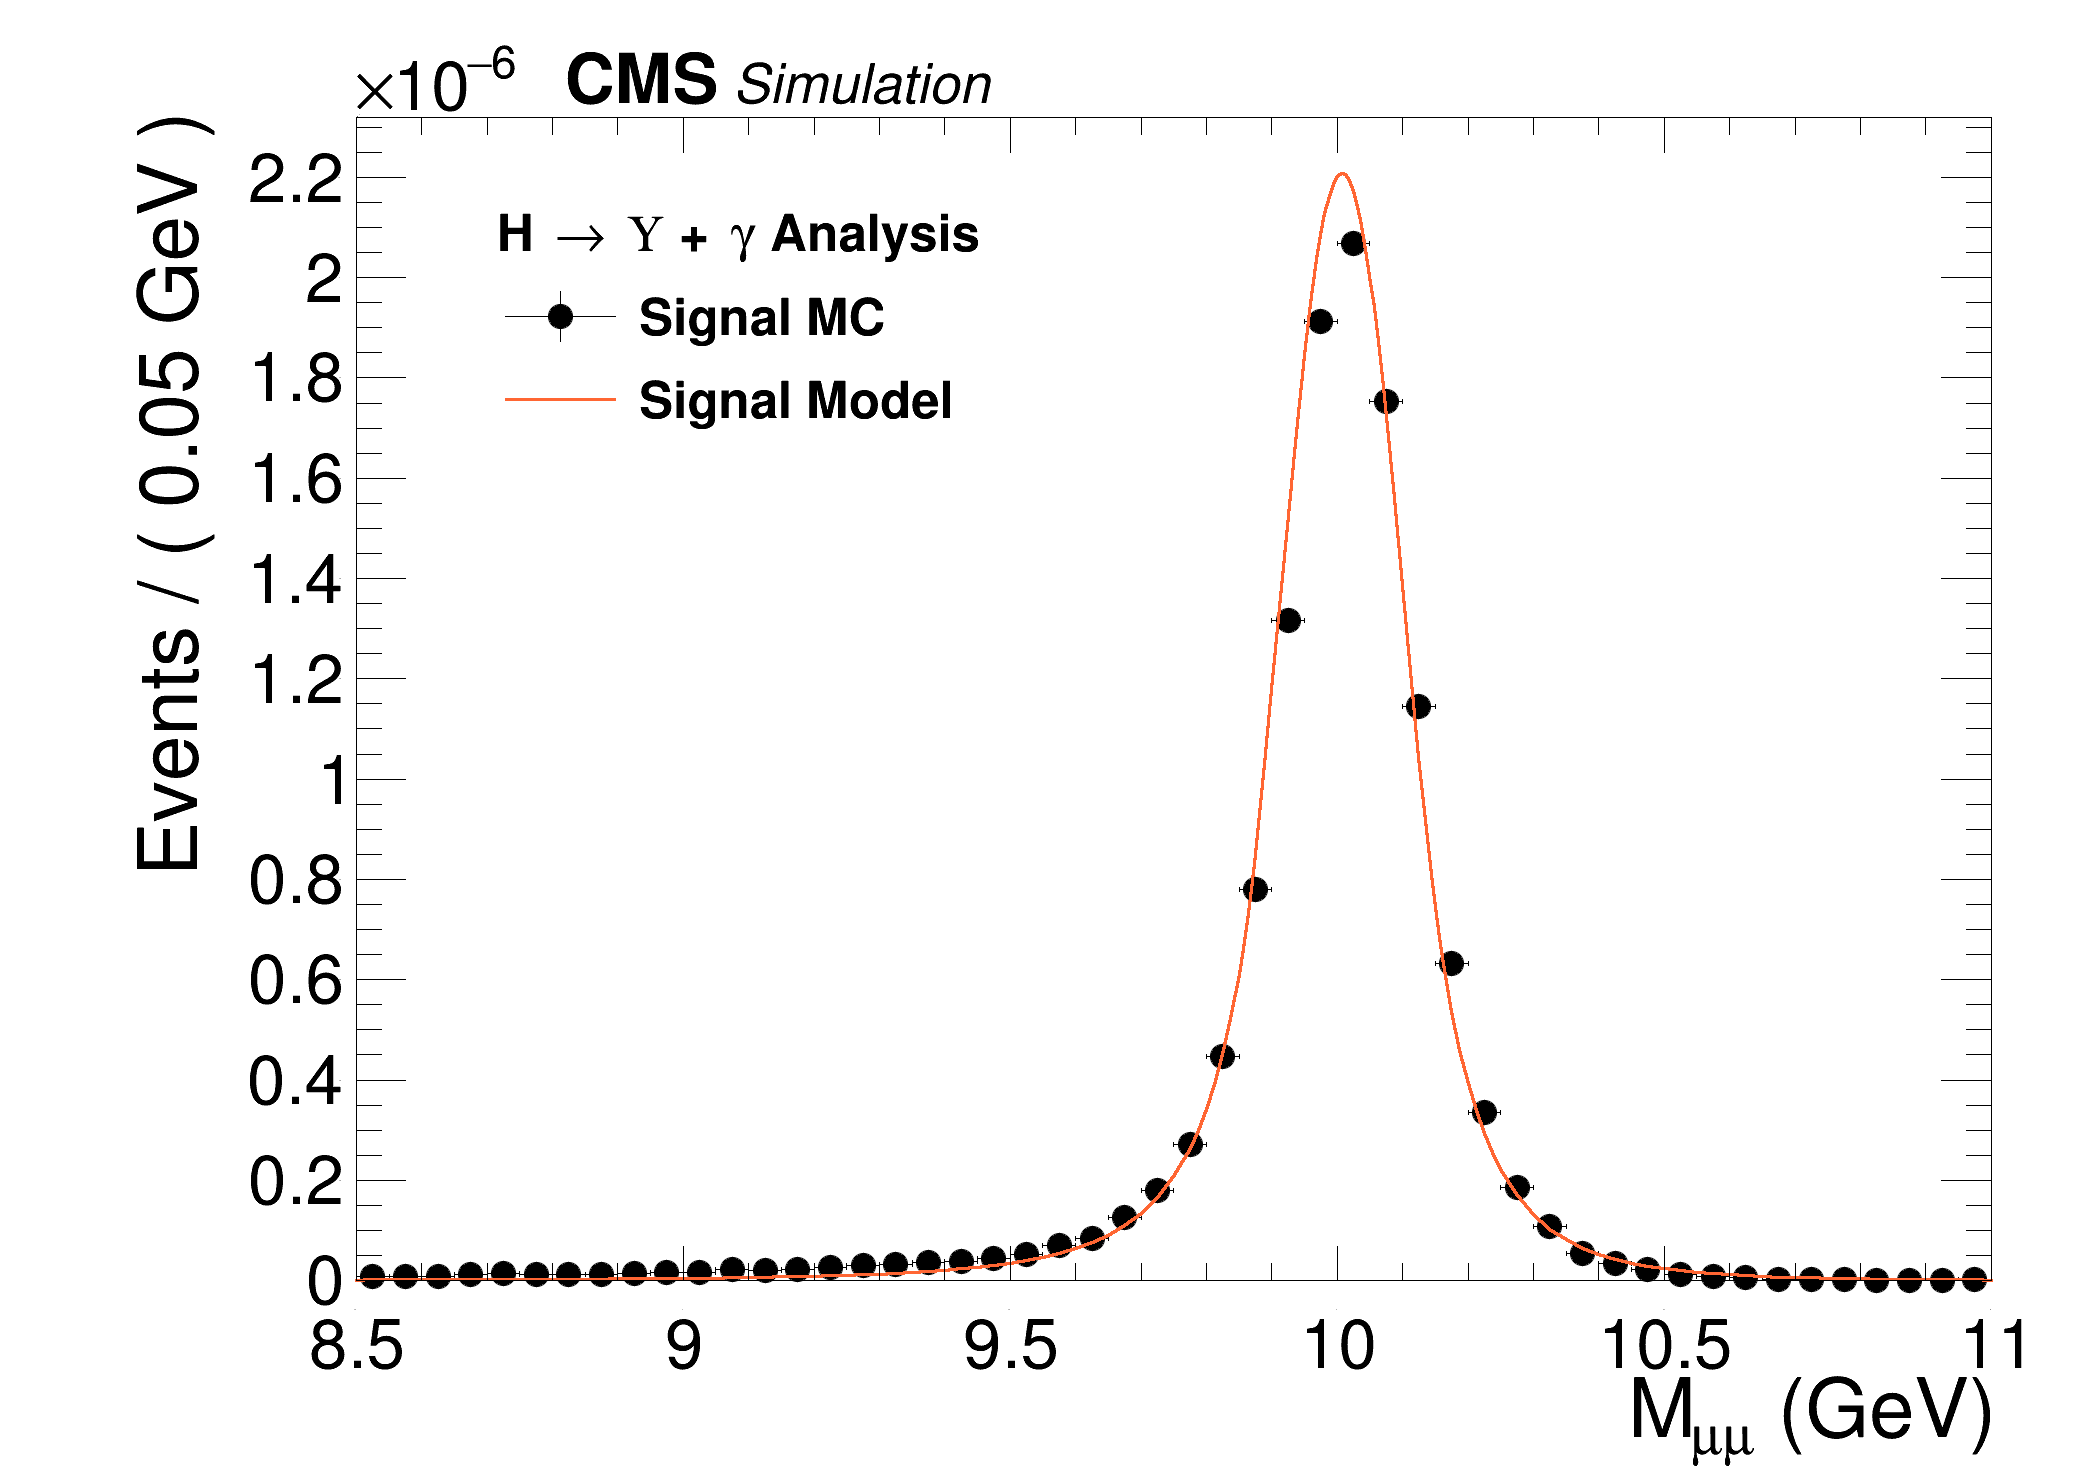
\includegraphics[width=0.45\textwidth]{figures_and_tables/fitPlotFiles2D/HToUpsilonPhotonSignalAndBackgroundFit/mMuMNU_HToUpsilon2SPhotonSignalAndBackgroundFit_Signal_Cat0}\hspace*{1.cm}
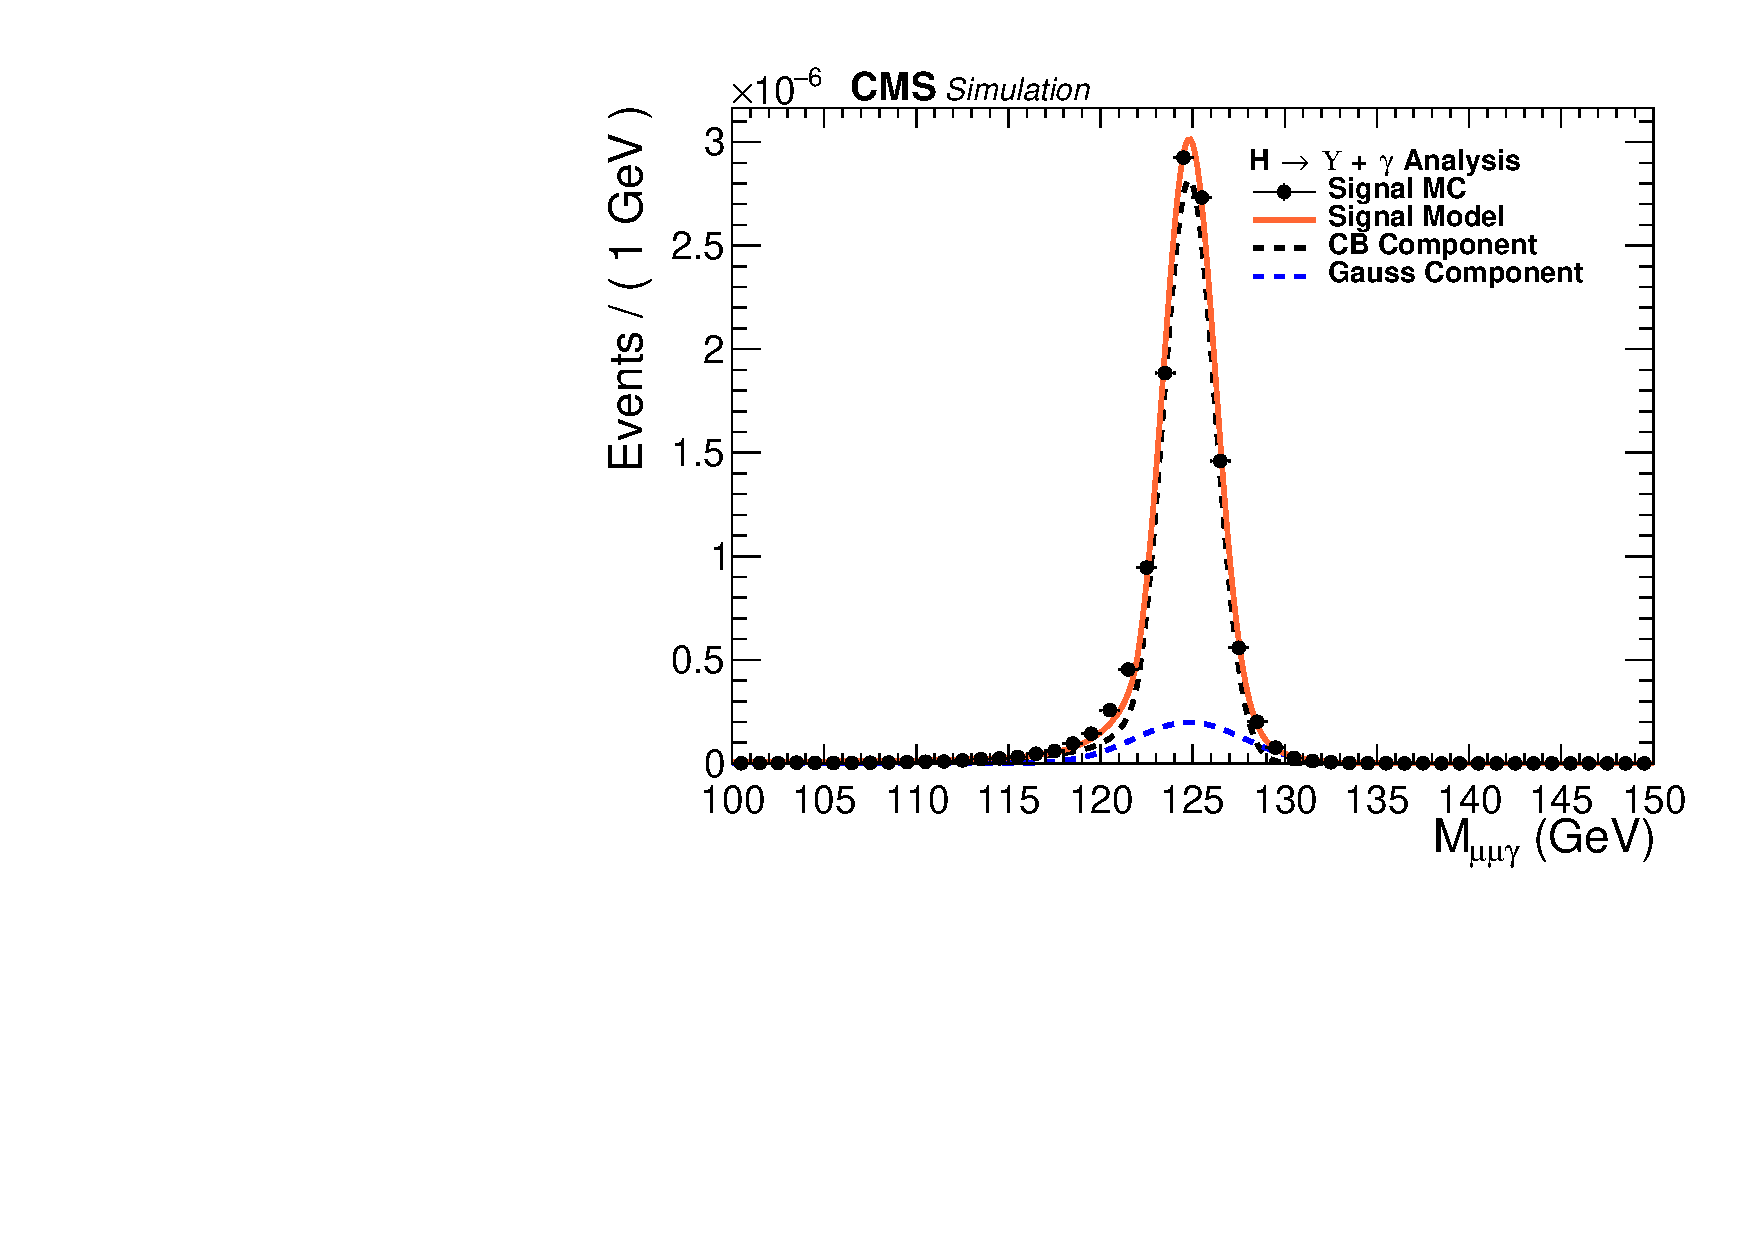
\includegraphics[width=0.45\textwidth]{figures_and_tables/fitPlotFiles2D/HToUpsilonPhotonSignalAndBackgroundFit/mHZ_HToUpsilon2SPhotonSignalAndBackgroundFit_Signal_Cat0_default}\hspace*{1.cm}

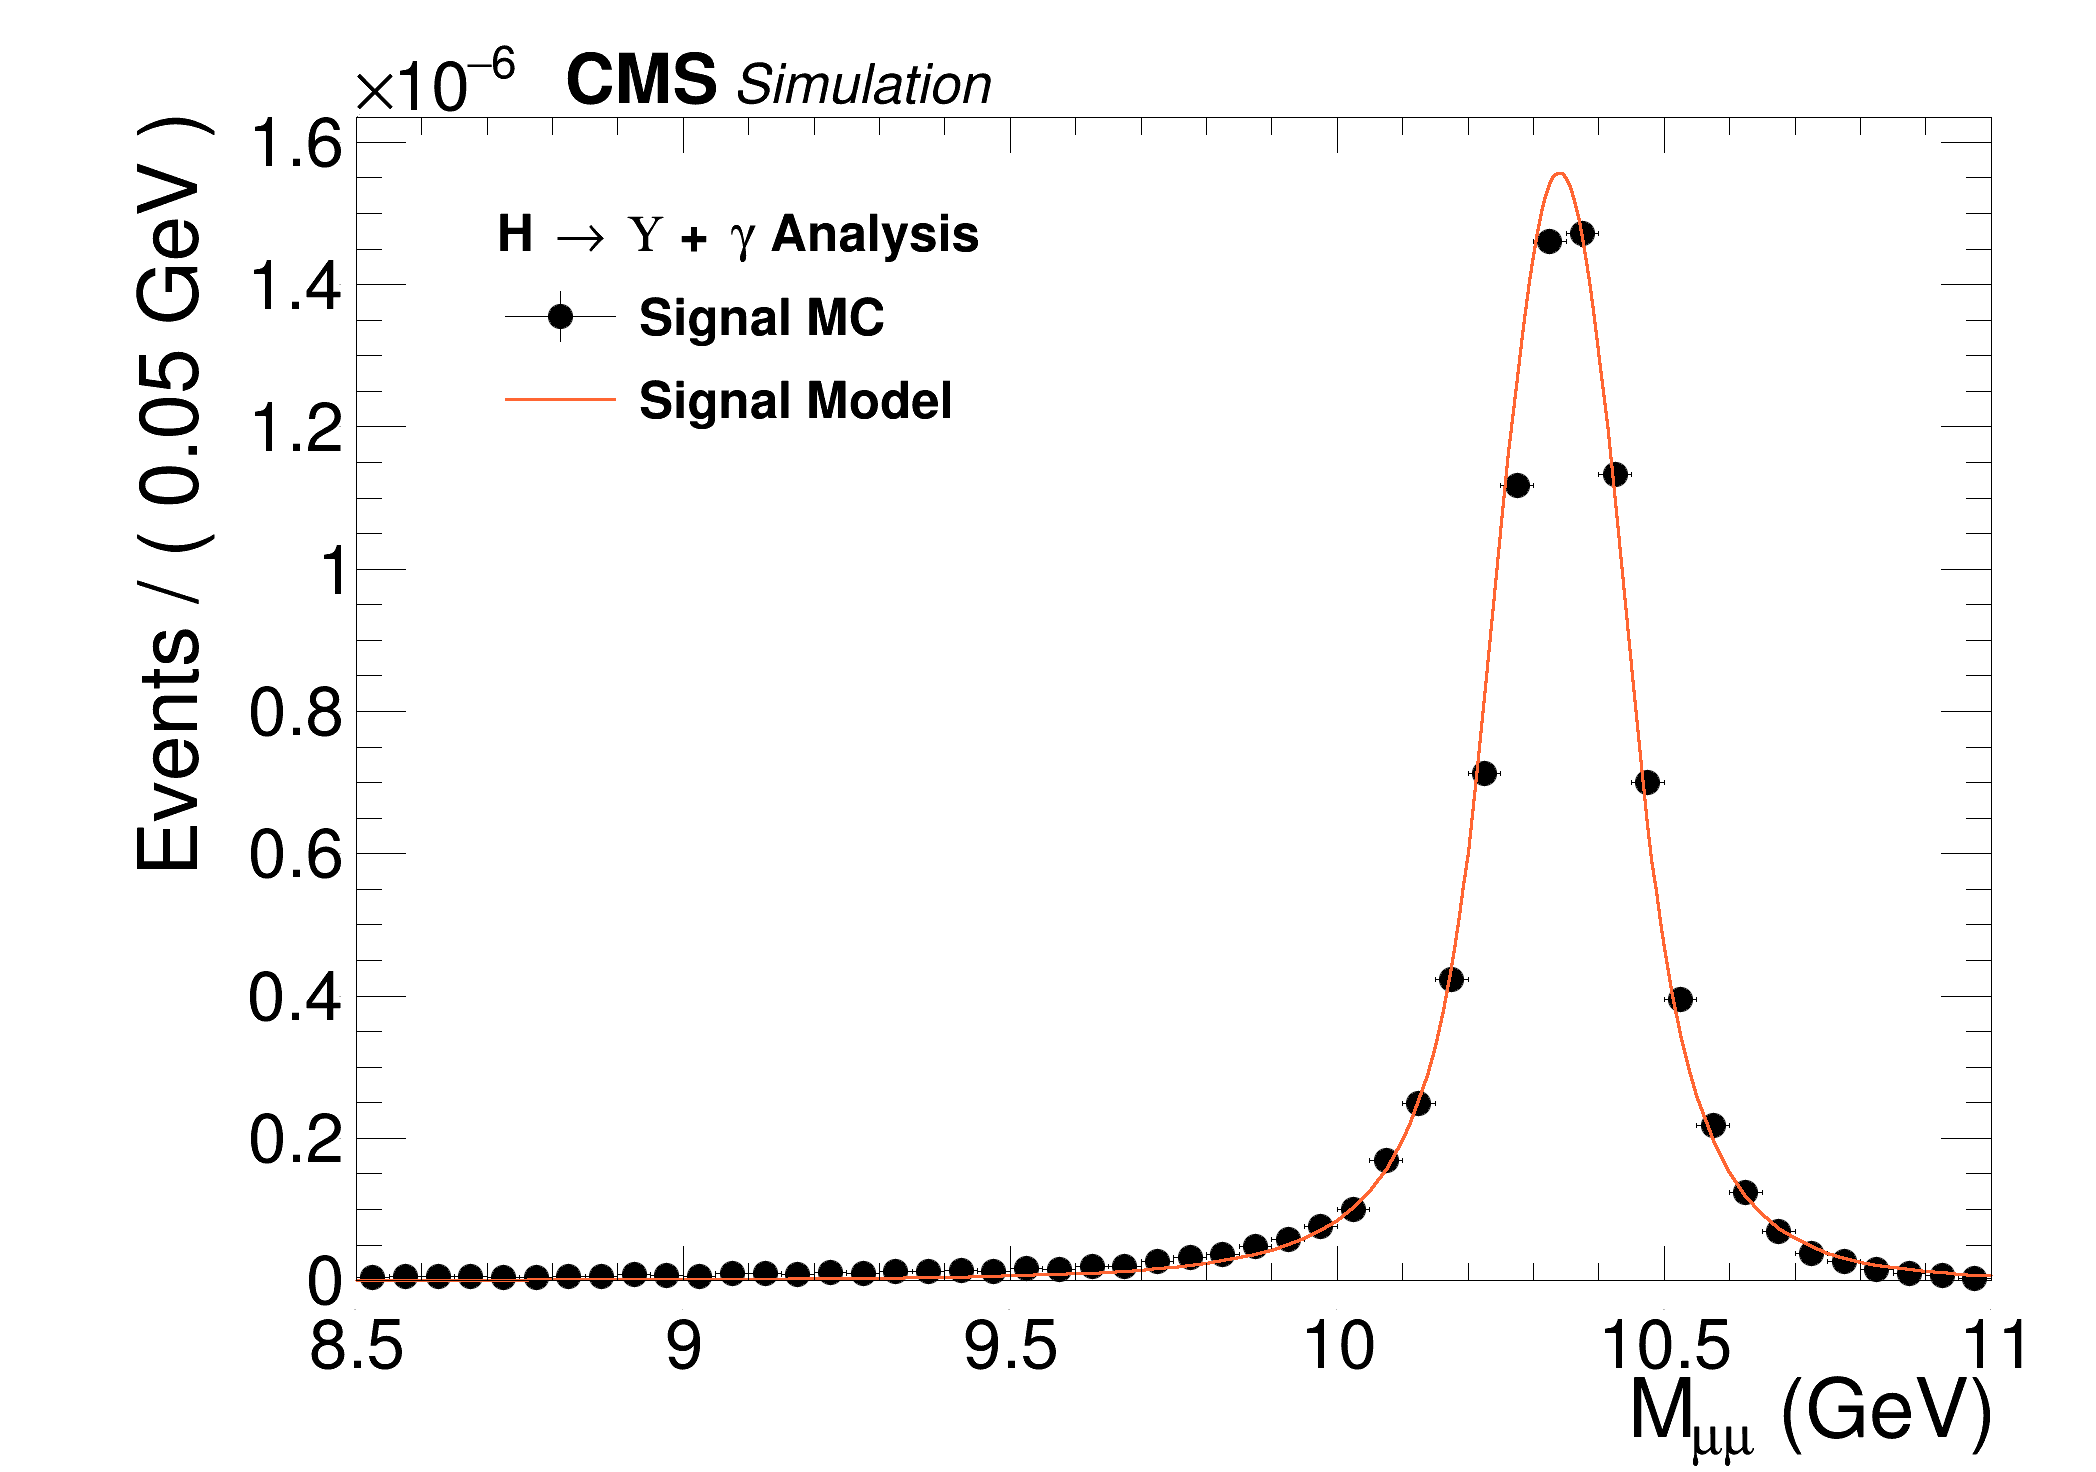
\includegraphics[width=0.45\textwidth]{figures_and_tables/fitPlotFiles2D/HToUpsilonPhotonSignalAndBackgroundFit/mMuMNU_HToUpsilon3SPhotonSignalAndBackgroundFit_Signal_Cat0}\hspace*{1.cm}
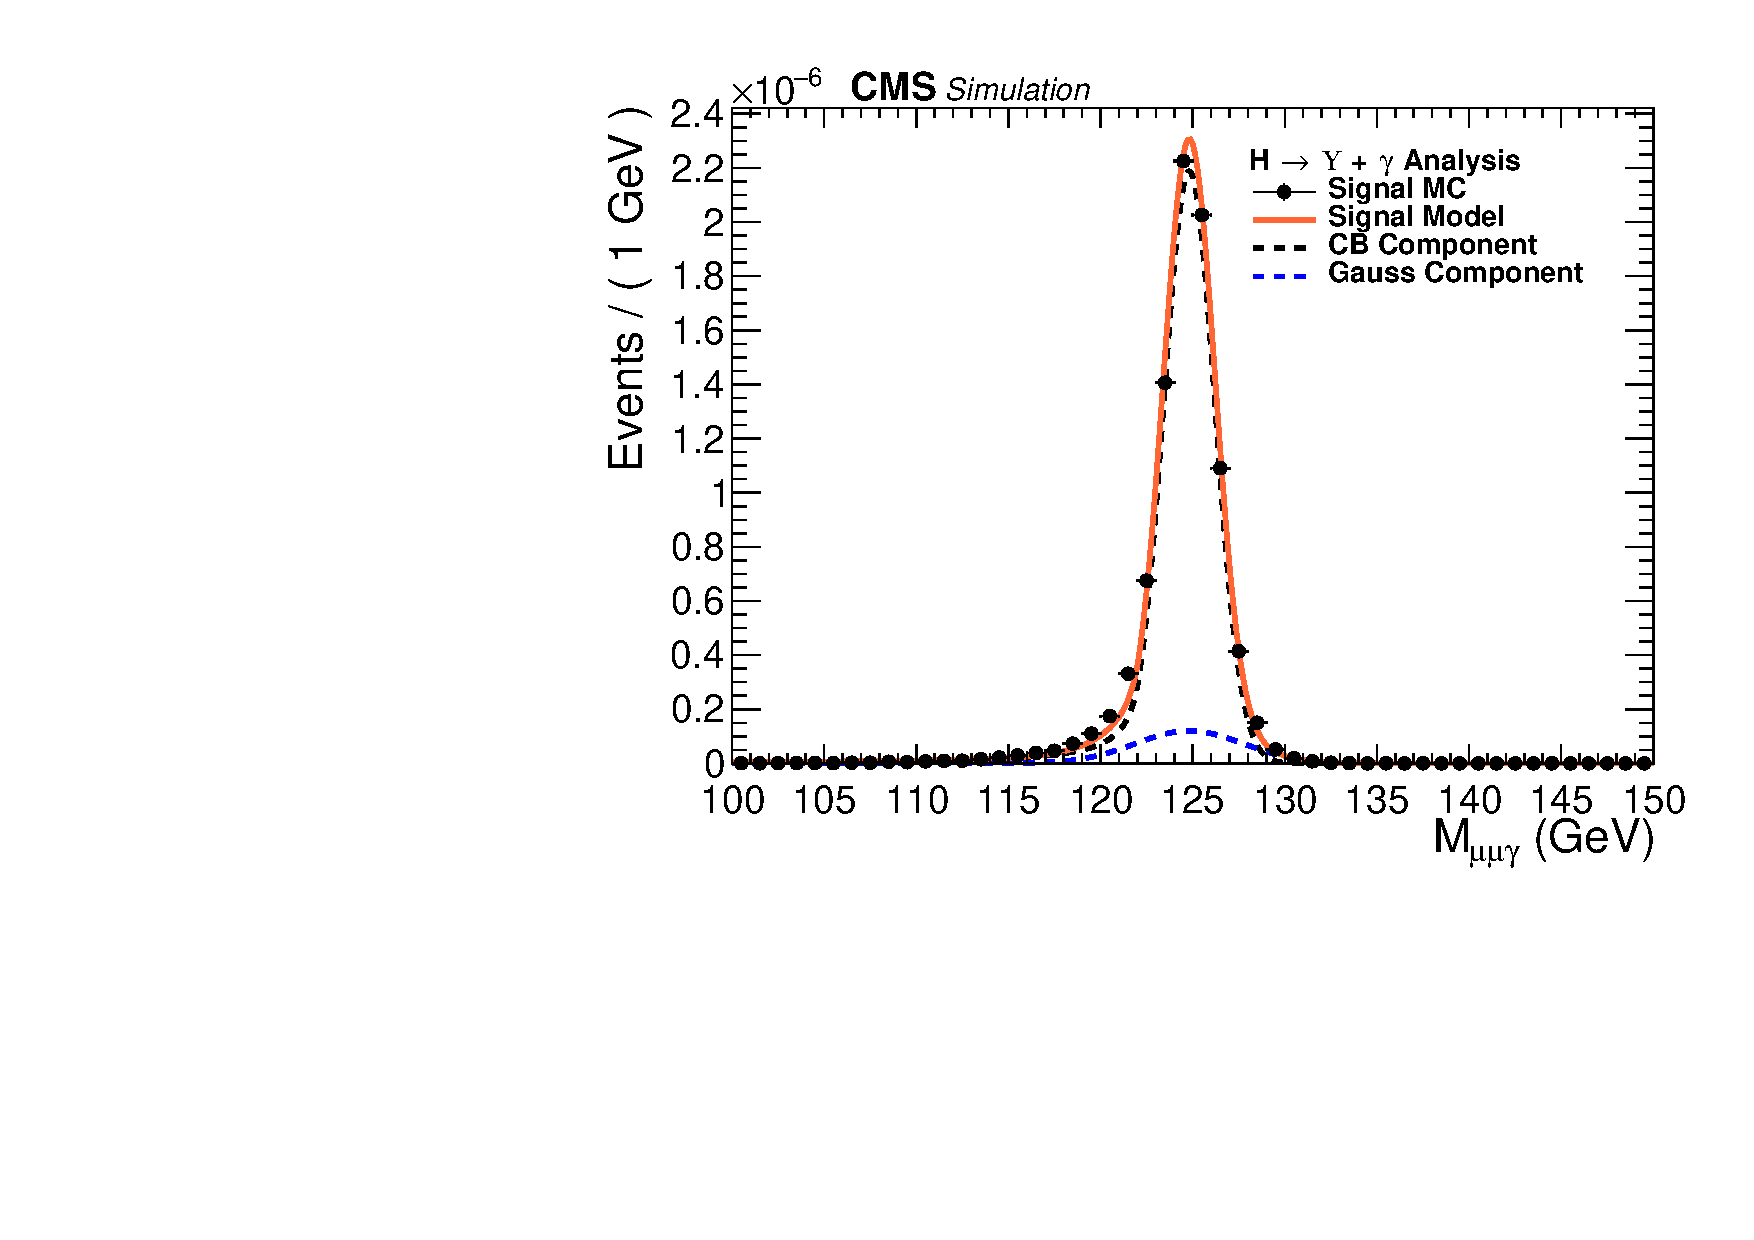
\includegraphics[width=0.45\textwidth]{figures_and_tables/fitPlotFiles2D/HToUpsilonPhotonSignalAndBackgroundFit/mHZ_HToUpsilon3SPhotonSignalAndBackgroundFit_Signal_Cat0_default}\hspace*{1.cm}


\end{center}\vspace*{-.5cm}
\caption{Signal Modeling for the $H \rightarrow \Upsilon(1S,2S,3S) +\gamma$. $m_{\mu\mu}$ mass distribution (left) and $m_{\mu\mu\gamma}$ mass distribution (right). From top to bottom: $\Upsilon(1S)$, $\Upsilon(2S)$, $\Upsilon(3S)$.}
\label{fig:HToUpsilon_Signal_Cat0}
\end{figure}

\clearpage
